% This is LLNCS.DEM the demonstration file of
% the LaTeX macro package from Springer-Verlag
% for Lecture Notes in Computer Science,
% version 2.4 for LaTeX2e as of 16. April 2010
%
\documentclass{llncs}
%
\usepackage{makeidx}  % allows for indexgeneration
% For figures
\usepackage{graphicx} % more modern
%\usepackage{epsfig} % less modern

\usepackage{subcaption}
\usepackage{color}
%\usepackage{subfig}%[caption=false,font=footnotesize]

% For citations
\usepackage{natbib}

% For algorithms
\usepackage{algorithm}
\usepackage{algorithmic}
\usepackage{amsmath}
% As of 2011, we use the hyperref package to produce hyperlinks in the
% resulting PDF.  If this breaks your system, please commend out the
% following usepackage line and replace \usepackage{icml2012} with
% \usepackage[nohyperref]{icml2012} above.
\usepackage{hyperref}

% Packages hyperref and algorithmic misbehave sometimes.  We can fix
% this with the following command.
\newcommand{\theHalgorithm}{\arabic{algorithm}}

%-------------------------------------------------------------
%                      Own Commands
%-------------------------------------------------------------
\usepackage{amsmath}
\newcommand{\cbn}{\textsc{Cbn}}
\newcommand{\bn}{\textsc{Bn}}
\newcommand{\huang}[1]{\textcolor{blue}{#1}}
\newcommand{\mycomment}[1]{\textcolor{red}{( ...#1 )}}
\renewcommand{\algorithmiccomment}[1]{/* #1 */}
\def\ci{\perp\!\!\!\perp}
\def\dep{\perp\!\!\!\perp\!\!\!\!\!\!\!/\,\,\,\,}
% Theorem & Co environments and counters
%\newtheorem{theorem}{Theorem}[section]
%\newtheorem{lemma}[theorem]{Lemma}
%\newtheorem{corollary}[theorem]{Corollary}
%\newtheorem{remark}[theorem]{Remark}
%\newtheorem{definition}[theorem]{Definition}
\newtheorem{equat}[theorem]{Equation}
%\newtheorem{example}[theorem]{Example}
%-------------------------------------------------------------

\begin{document}
%
\frontmatter          % for the preliminaries
%
%\pagestyle{headings}  % switches on printing of running heads
%\addtocmark{Hamiltonian Mechanics} % additional mark in the TOC
%%
%\tableofcontents
%
\mainmatter              % start of the contributions
%
\title{ Communication-efficient Learning from Multiple Experts}
%
%\titlerunning{Hamiltonian Mechanics}  % abbreviated title (for running head)
%                                     also used for the TOC unless
%                                     \toctitle is used
%
\author{Bojan  Kolosnjaji\inst{1} \and Huang Xiao\inst{2} 
	\and Claudia Eckert\inst{1}\inst{2} }
%Jeffrey Dean \and David Grove \and Craig Chambers \and Kim~B.~Bruce \and
%Elsa Bertino}
%
\authorrunning{Bojan Kolosnjaji et al.} % abbreviated author list (for running head)
%
%%%% list of authors for the TOC (use if author list has to be modified)
%\tocauthor{Ivar Ekeland, Roger Temam, Jeffrey Dean, David Grove,
%Craig Chambers, Kim B. Bruce, and Elisa Bertino}
%
\institute{Technical University of Munich, Fraunhofer AISEC\\
\email{kolosnjaji@sec.in.tum.de, huang.xiao@aisec.fraunhofer.de, eckert@sec.in.tum.de}
%\\ WWW home page:
%\texttt{https://www.aisec.fraunhofer.de/}
%\and
%Universit\'{e} de Paris-Sud,
%Laboratoire d'Analyse Num\'{e}rique, B\^{a}timent 425,\\
%F-91405 Orsay Cedex, France
}

\maketitle              % typeset the title of the contribution

\begin{abstract}
Learning from multiple sources of labeled data can increase the confidence of a machine learning system if the expertise of different labelers can be assembled efficiently. However, using a large amount of labelers in the test time can be expensive in the long run. For instance, in crowdsourcing, we have to pay each labeler in order to get the annotations. In Internet-of-Things, obtaining data from multiple sensors for direct fusion incurs high communication overhead. 

In this paper, we propose a method for training a classification system from data labeled by multiple client annotators, where only a small subset of annotators are optimally chosen to reduce communication effort. 
We define an iterative optimization procedure where the sparsity of a client weight vector is enforced while reducing the overall classification error. Using a set of experiments with real and synthetic data, we show that our approach can pertain the classification performance as on the complete set of labelers while reducing the communication effort by over 70\% on several different tasks.

\keywords{machine learning, communication-efficiency, crowdsourcing, Internet-of-Things}
\end{abstract}
%

\section{Introduction}
Supervised machine learning depends on our ability to gather a large set of labeled data. In a high number of scenarios, we can benefit from labeled data gathered by querying multiple separate sources with varying reliability and join this data into one machine learning model. However, many times we are limited in the number of data sources that we are allowed to use, because of budget constraints, limited processing power or insufficient communication bandwidth. This causes the need for a framework that would enable resource-efficient combination of labeled data from multiple sources.

First important fitting scenario to this framework is crowdsourcing. When using crowdsourcing systems such as Amazon Mechanical Turk, we can gather labelled data from multiple annotators. After gathering this training data, we need to join the labelling decisions and train one machine learning system while leveraging all of the annotations. Relying on a concept of \textit{wisdom of crowds}, we can assume that if we gather data from a sufficient number of people, on average most of them will give correct labelling decision. However, gathering data from a large amount of annotators can be expensive, as workers on Amazon Mechanical Turk require payment for their work. Therefore we would benefit from a procedure of prior determination of the annotators' expertise. In this case, the joining process can be optimized by estimating the expertise of the annotators, selecting the optimal subset and determining weights of the annotators' labels. Moreover, in a rising area of \textit{Internet of Things} (IoT) we can have similar problems. In IoT systems, a large number of sensors provide information about the environment. Communication among multiple sensors can be costly in terms of processing power. Furthermore, this communication can be done among sensors that are limited with power consumption constraints. Furthermore, in intrusion detection it is useful to use results from multiple anomaly detection systems. For example, although there are multiple antivirus programs that can label software as benign or malicious programs of certain type, only a minority of the programs contain updated labels for newest malware families and classify malware with high granularity. Therefore it would be useful to find a subset of label sources that are reliable enough to be used for malware triage purposes.

There are multiple papers that deal with estimating the expertise of labelers when using \textit{wisdom of crowds}. For example, Welinder et al. \cite{welinder2010multidimensional} determine groups of annotators with similar expertise, and find particular phenomena such as "schools of thought" and specialist experts in certain types of image labeling tasks. Tian and Zhu~\cite{tian2012learning} investigate the annotator behavior in executing more complex labeling tasks, such as answering if an image is beautiful or if it contains a car. Zhang et al.~\cite{zhang2013learning} propose a method to filter out novice labelers. However, their method is specific to Gaussian Mixture Models. Rodrigues et al.~\cite{rodrigues2014gaussian} determine a similar procedure specific to Gaussian Processes. Bi et al.~\cite{bi2014learning} argue that the factors that determine the annotators' labeling performance, apart from the expertise, can also be the worker's dedication to the task, his/her default labeling judgement and sample difficulty. However, they do not go further in determining the optimal subset of annotators. On the other hand, Li and Liu~\cite{li_liu_2015} propose a combinatiorial procedure to find this optimal subset. However, such combinatorial procedures are very resource-intensive, especially for a large initial set of annotators.

On the other hand, there are are also multiple more theoretical frameworks. For example, Wang et al.~\cite{wang2015efficient} propose a selection of sensors based on Directed Acyclic Graphs (DAGs) in resource-constrained scenarios. However, they do not deal with annotating data, so their ideas do not completely fit to our problem. 

We design a methodology that both selects an optimal subset of annotators from a set of training data and automatically determines the weights of the selected annotators. By forcing sparsity on our annotator weight vector during optimization, we get an accurate classification system that works well even with annotations from a small set of highly competent annotators. This gives us a low-budget supervised learning strategy, which is not specific to any particular learning algorithm.

In summary, we make the following contributions:
\begin{itemize}
\item We propose a methodology for selecting an optimal subset of workers in a classification system with multiple labelers
\item We create a procedure for selecting and determining weights of labelers independent of the type of machine learning methods selected for modeling the annotating process
\item Using a set of experiments with both real and synthetic data, we show that we can obtain an accurate classification system with the optimized annotator subset.
\end{itemize}  


\section{Methodology}

Our methodology is based on the scenario drawn on the \autoref{fig:scheme}. This scheme shows a common situation when a server acquires labels from multiple annotators. 

\begin{figure}
  \caption{Label aggregation scheme}
  \centering
    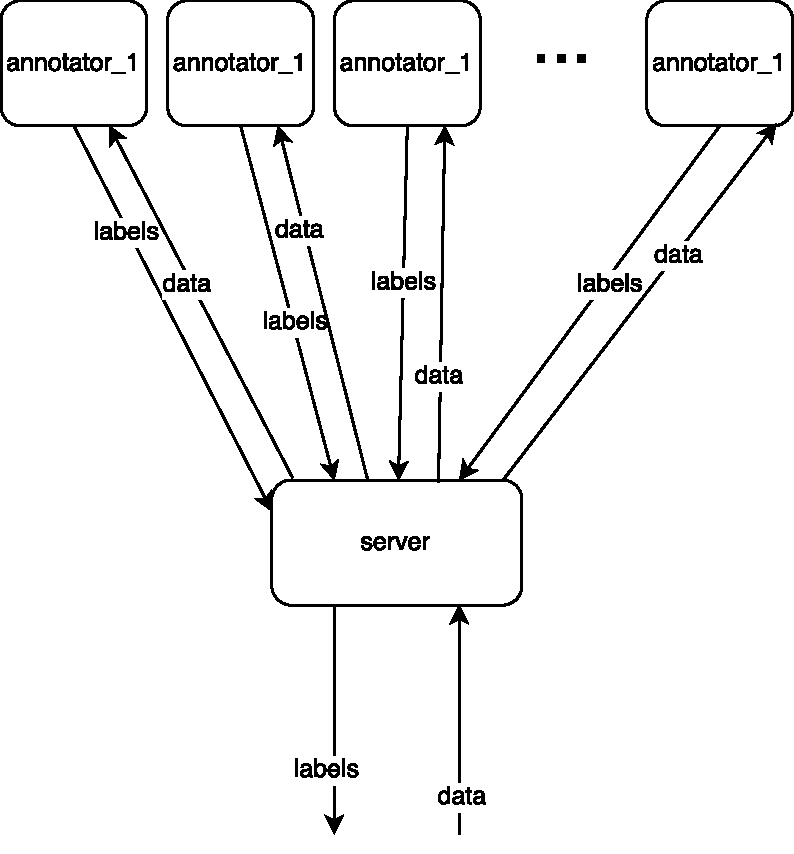
\includegraphics[width=0.5\textwidth]{figures/lowbudget.pdf}
  \label{fig:scheme}
\end{figure}

In training time, server forwards the training inputs to all the annotators in order to retrieve labels. Using the data labeled from a large set of annotators, the server trains a machine learning model that jointly learns the expertise of all the clients while minimizing the quadratic loss with respect to the ground truth.  

We design a method that would enable us to manage the tradeoff between model accuracy and communication effort. Furthermore, we impose a requirement that our methodology needs to be simple and compatible with a wide range of machine learning methods. 

Based on these requirements, our optimization model has a cost function consisting of three parts:

\begin{enumerate}
\item minimizing the cost with respect to the ground truth labels on the training set
\item minimizing the cost with respect ot the client annotations
\item making the client weight vector sparse (select a small subset of clients)
\end{enumerate}

The cost function for cross-entropy loss on ground truth, used in all our experiments, looks like the following:

\begin{equation}
\begin{split}
 L(w,v)= -\frac{1}{N} \sum_{n=1}^N (\hat{y}_n \log \sum_{i=1}^M v_i y_{ni} + (1-\hat{y}_n) \log(1-\sum_{i=1}^M v_i y_{ni})) + \\ + \psi \sum_{i=1}^{M} (y_{ni} - z_{ni})^2+\lambda \mid v \mid
\end{split} 
\end{equation}
subject to:
\begin{equation}
 \sum_{i=1}^{M} v_i = 1 
\end{equation}

\noindent where $ \hat{y}_n $ are ground truth labels for all training samples, $ y_{ni} $ are labels retrieved by querying  current client models, $z_{ni}$ are training labels from annotator clients, $v_i$ is a normalized vector of weights for all the clients. The final loss function consists of a crossentropy calculation for the empirical loss with respect to the ground truth, the quadratic loss with respect to the client annotations weighted by a parameter $\phi$ and the $L_1$-norm of the parameter vector $v$ weighted by another parameter $\lambda$.

We want to use $L_1$ regularization to minimize the client weight vector. This is similar to the \textit{Lasso} feature selection, except that we select clients instead of features. 

The gradient is defined with the following equations:
\begin{equation}
\begin{split}
 \frac{\partial L}{\partial w_j} = -\frac{1}{N} \sum_{n=1}^N (y_n \frac{1}{\sum_{i=1}^M v_i \hat{y}_{ni}} v_j \frac{\partial y_n}{\partial w_j} + (1-y_n) \frac{1}{1-\sum_{i=1}^M } v_j \frac{\partial y_n}{\partial w_j} + \\  \psi \sum_{i=1}^M 2 (y_{ni} - z_{ni} \frac{\partial y_n}{\partial w_j}  ))
\end{split}
\end{equation}

\begin{equation} \frac{\partial L}{\partial v_i} =  -\frac{1}{N} \sum_{n=1}^N (y_n \frac{1}{\sum_{i=1}^M v_i y_{ni}} + (1-\hat{y_n}) \frac{1} {1-\sum_{i=1}^M v_i y_{ni}} (-y_n) 
\end{equation}
The expression for the gradient $ \frac{\partial y_n}{\partial w_j}$ depends on the concrete method used to model the annotators.

For logistic regression we directly define the cost for the errors with respect to ground truth as crossentropy. However, with minimal changes our framework can also be usable with other machine learning methods. For example, we tested our methodology with neural networks as well, using a perceptron with one hidden layer. These methods, however, need to be convex or have a convex relaxation in order to still make a gradient-based optimization procedure work well.

In order to still use gradient descent as a convex optimization method with the $L_1$ norm, we use iterative soft-thresholding~\cite{bredies2007iterative}, a type of generalized gradient descent optimization when updating the value of $v$. The update that we derived is the following:

\begin{equation}
 v= v + S_{\lambda} (v-t_s \frac{\partial L}{\partial v}, \lambda)
\end{equation}
where
\begin{equation}
S_{\lambda} (k, \lambda) = 
\left\{
	\begin{array}{ll}
		k-\lambda  & \mbox{if } k > \lambda  \\
		k+\lambda & \mbox{if } k < -\lambda \\
		0 & \mbox{otherwise}
	\end{array}
\right.
\end{equation}

Furthermore, we normalize the values in the vector $v$ in order to retrieve the proper values of client weights:

\begin{equation}
v = \frac{v}{\sum_{i=1}^M v_i}
\end{equation}

In case of multiclass classification, we define the loss function in a slightly different way, to accomodate with the fact that we need a label vector instead of scalar value:

\begin{equation}
 L(w,v)= -\frac{1}{N} \sum_{n=1}^N \sum_{k=1}^K (\hat{y}_{nk} \log \sum_{i=1}^M v_i y_{nik}) + \psi \sum_{i=1}^{M} (y_{ni} - z_{ni})^2+\lambda \mid v \mid
\end{equation}, 

subject to
\begin{equation}
 \sum_{i=1}^{M} v_i = 1 
\end{equation}

This time, $\hat{y}$ is a matrix and $y$ is a three-dimensional tensor. The optimization is done in a similar way, using projected gradient descent. We minimize the cross-entropy w.r.t the ground truth, as well as the squared difference of ground truth and annotator decision, while keeping the annotator vector sparse.

%Full expertise model:
%
%
%\begin{equation}
%\begin{split}
% L(w,v)= -\frac{1}{N} \sum_{n=1}^N (\hat{y}_n \log \sum_{i=1}^M v_{ni} y_{ni} + (1-\hat{y}_n) \log(1-\sum_{i=1}^M v_{ni} y_{ni})) + \\ \psi \sum_{i=1}^{M} (y_{ni} - z_{ni})^2+\sum_{n=1}^{N}\lambda \mid v_n \mid
%\end{split} 
%\end{equation}

\section{Results}

We use two datasets to evaluate our methodology of combining the expertise of different annotators. Furthermore, we test our approach using two different models of annotators: logistic regression model and a neural network model (perceptron with one hidden layer).

\subsection{Datasets}
In order to evaluate our approach, we use one dataset with real-life labelers and one with synthetic labelers. 

\subsubsection{Real-Life Labelers}
We obtained a real-life labeler set from the authors of a related paper about learning to predict from crowdsourced data by Bi et al.~\cite{bi2014learning}. This dataset consists of results from an experiment with 21 workers at the \textit{Amazon Mechanical Turk}. These workers executed 10 tasks, all of the tasks being binary classification of images. Since each worker has different expertise, the challenge is to determine the subset of highly competent workers and combine their abilities for a superior classification system.

\subsubsection{Synthetic Labelers}
In order to further examine the performance of our method, we also use a semi-synthetic data based on the well-known MNIST dataset~\cite{lecun1998mnist} for digit recognition with around 70000 images of digits. We use images from this data without change and we take labels for images as ground truth. However, we synthetically create annotators by training multiple classifiers with random 0.5\% of images from the original set. This gives us annotators that have expertise in labeling only a subset of images, that on average have 81\% accuracy on a holdout test set. We use this set of annotators to test if we can surpass the performance of a single particular annotator by combining a minority of them.

\subsection{Optimization process}

Furthermore, we look at how the value of the loss function changes while the optimization is running. We plot the loss against the number of iteration, which shows the steep decline of the loss value. This shows that using our gradient-based procedure we can get fast to a very accurate classification system. The graph is shown on \autoref{fig:optimization}.

Next, we execute a similar test with the parameter $v$. We look at how the number of nonzero elements of $v$ changes while optimization is running. In other words, we examine how the optimizer selects the competent annotators.

\begin{figure}[!htb]	
    \centering
    
    \begin{subfigure}[b]{0.45\textwidth}
        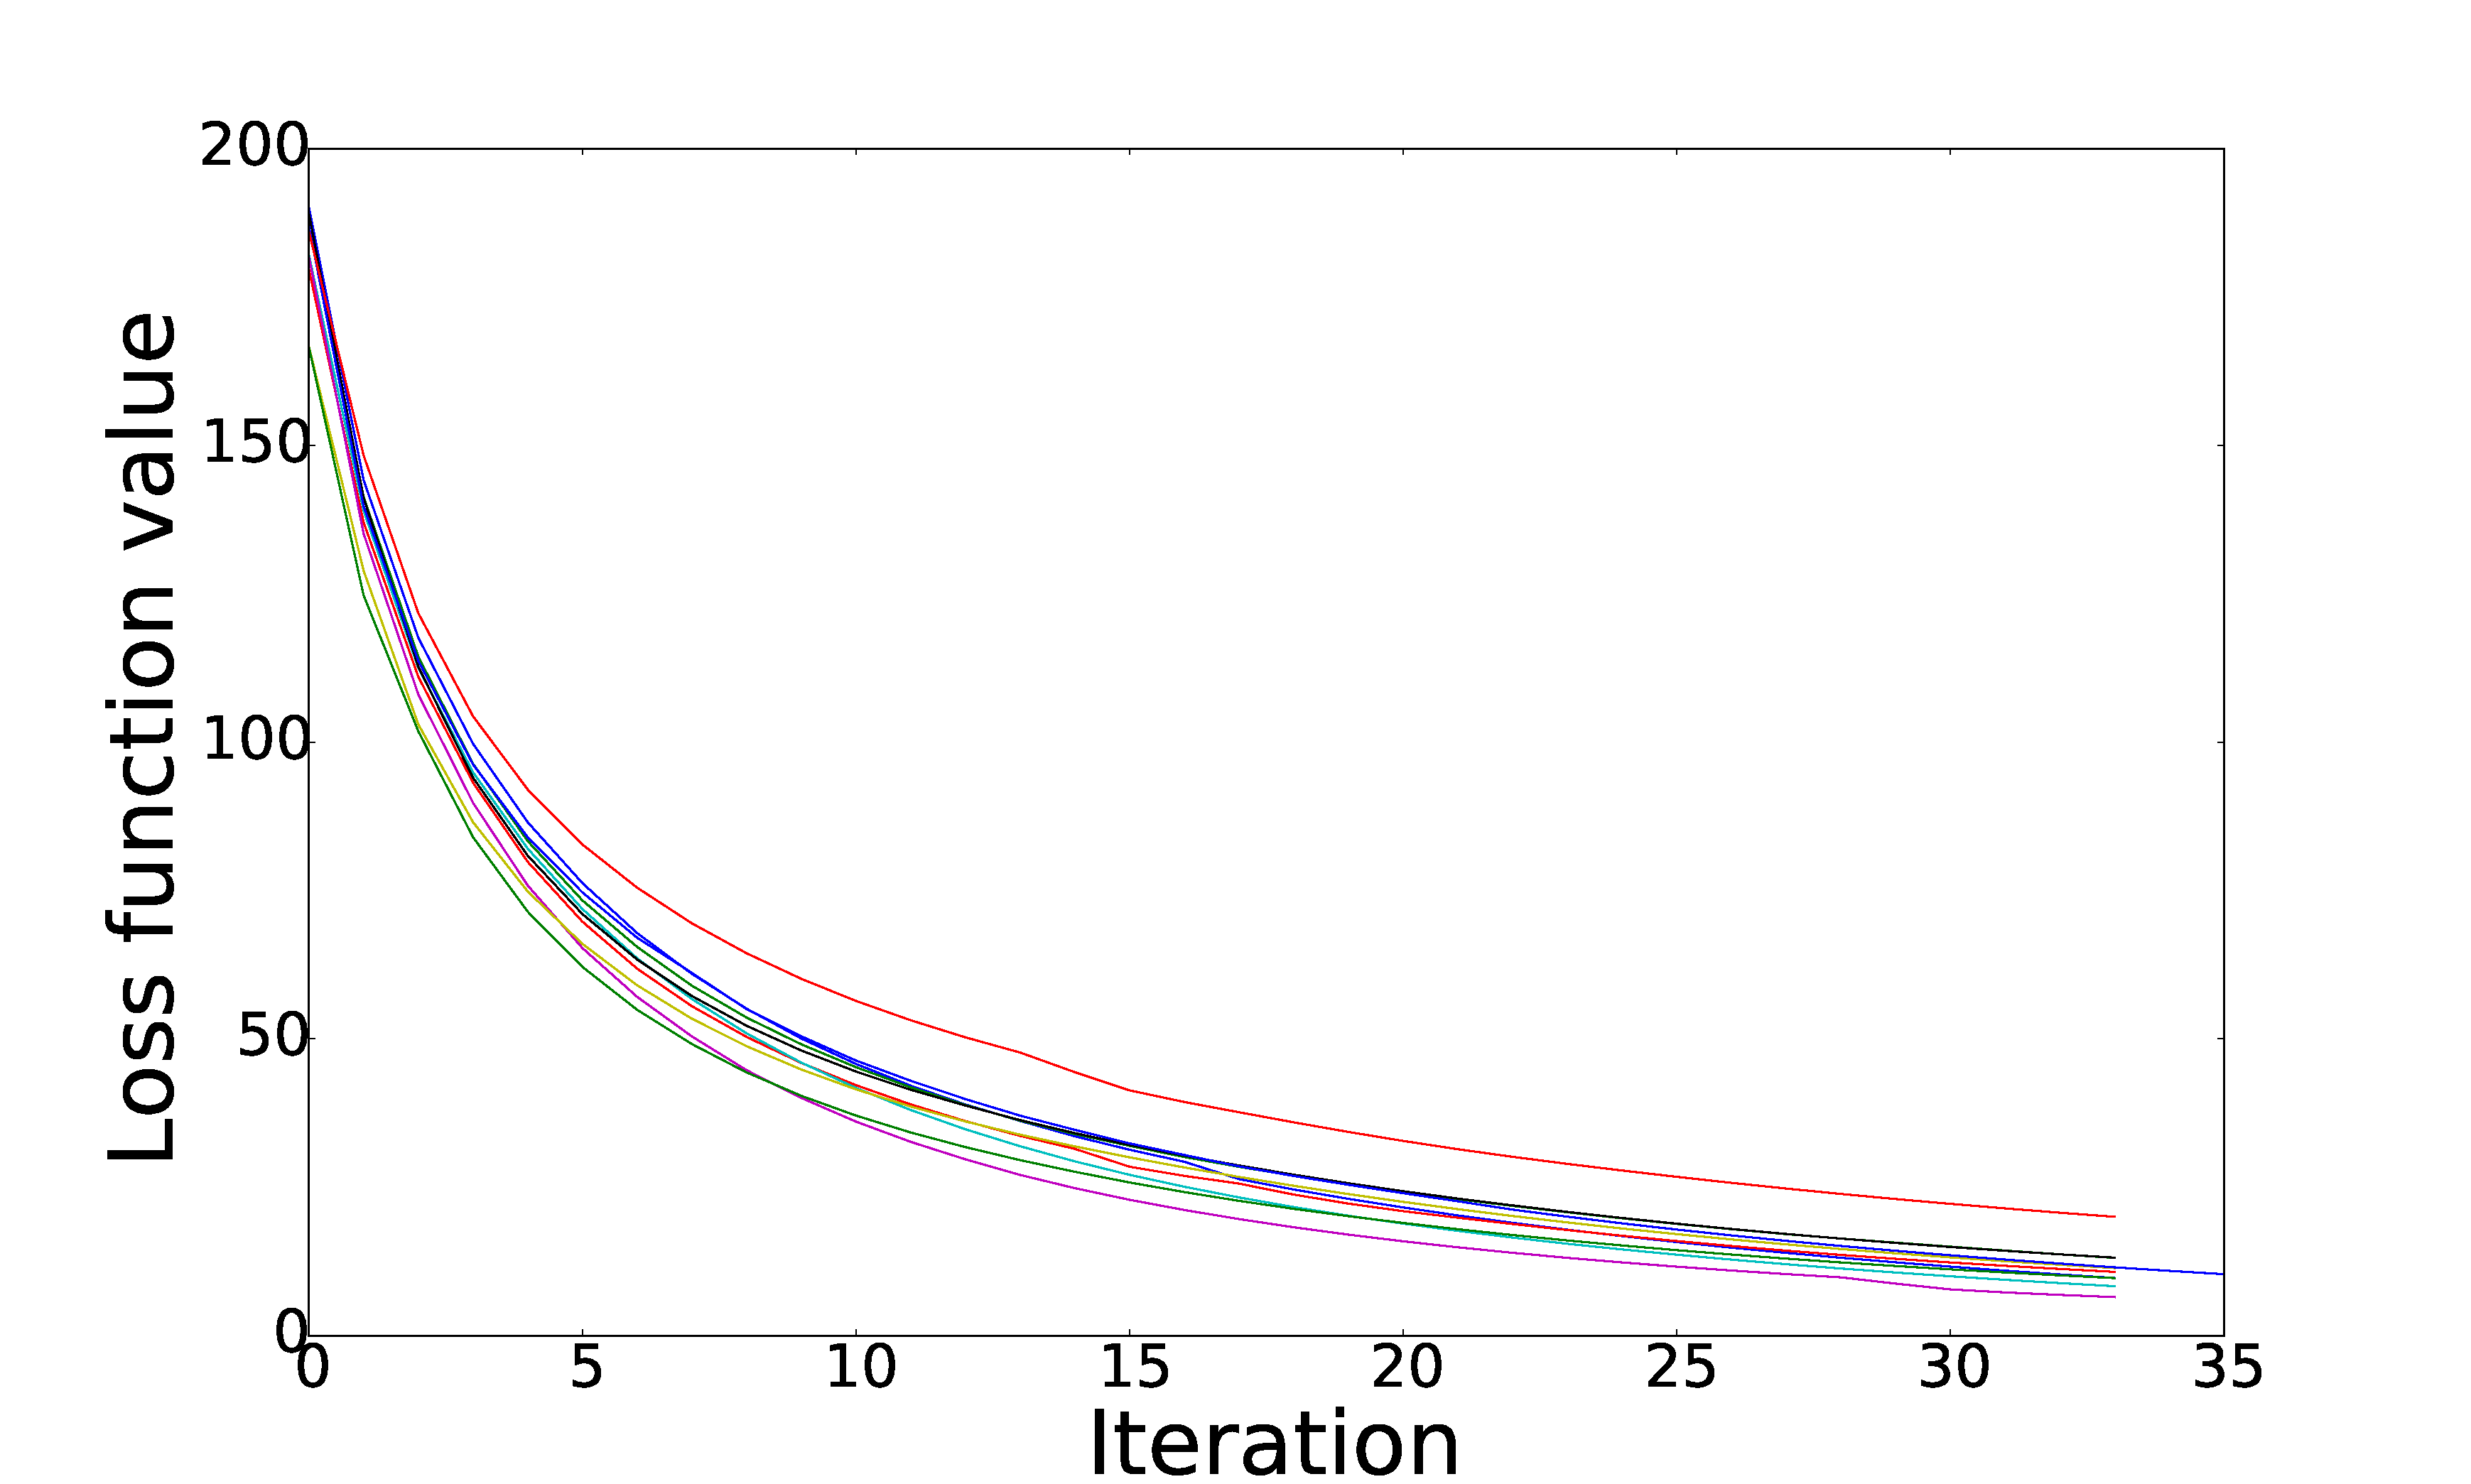
\includegraphics[width=\textwidth]{figures/loss_iteration_logreg}
        \caption{Loss minimization}

    \end{subfigure}
    \begin{subfigure}[b]{0.45\textwidth}
        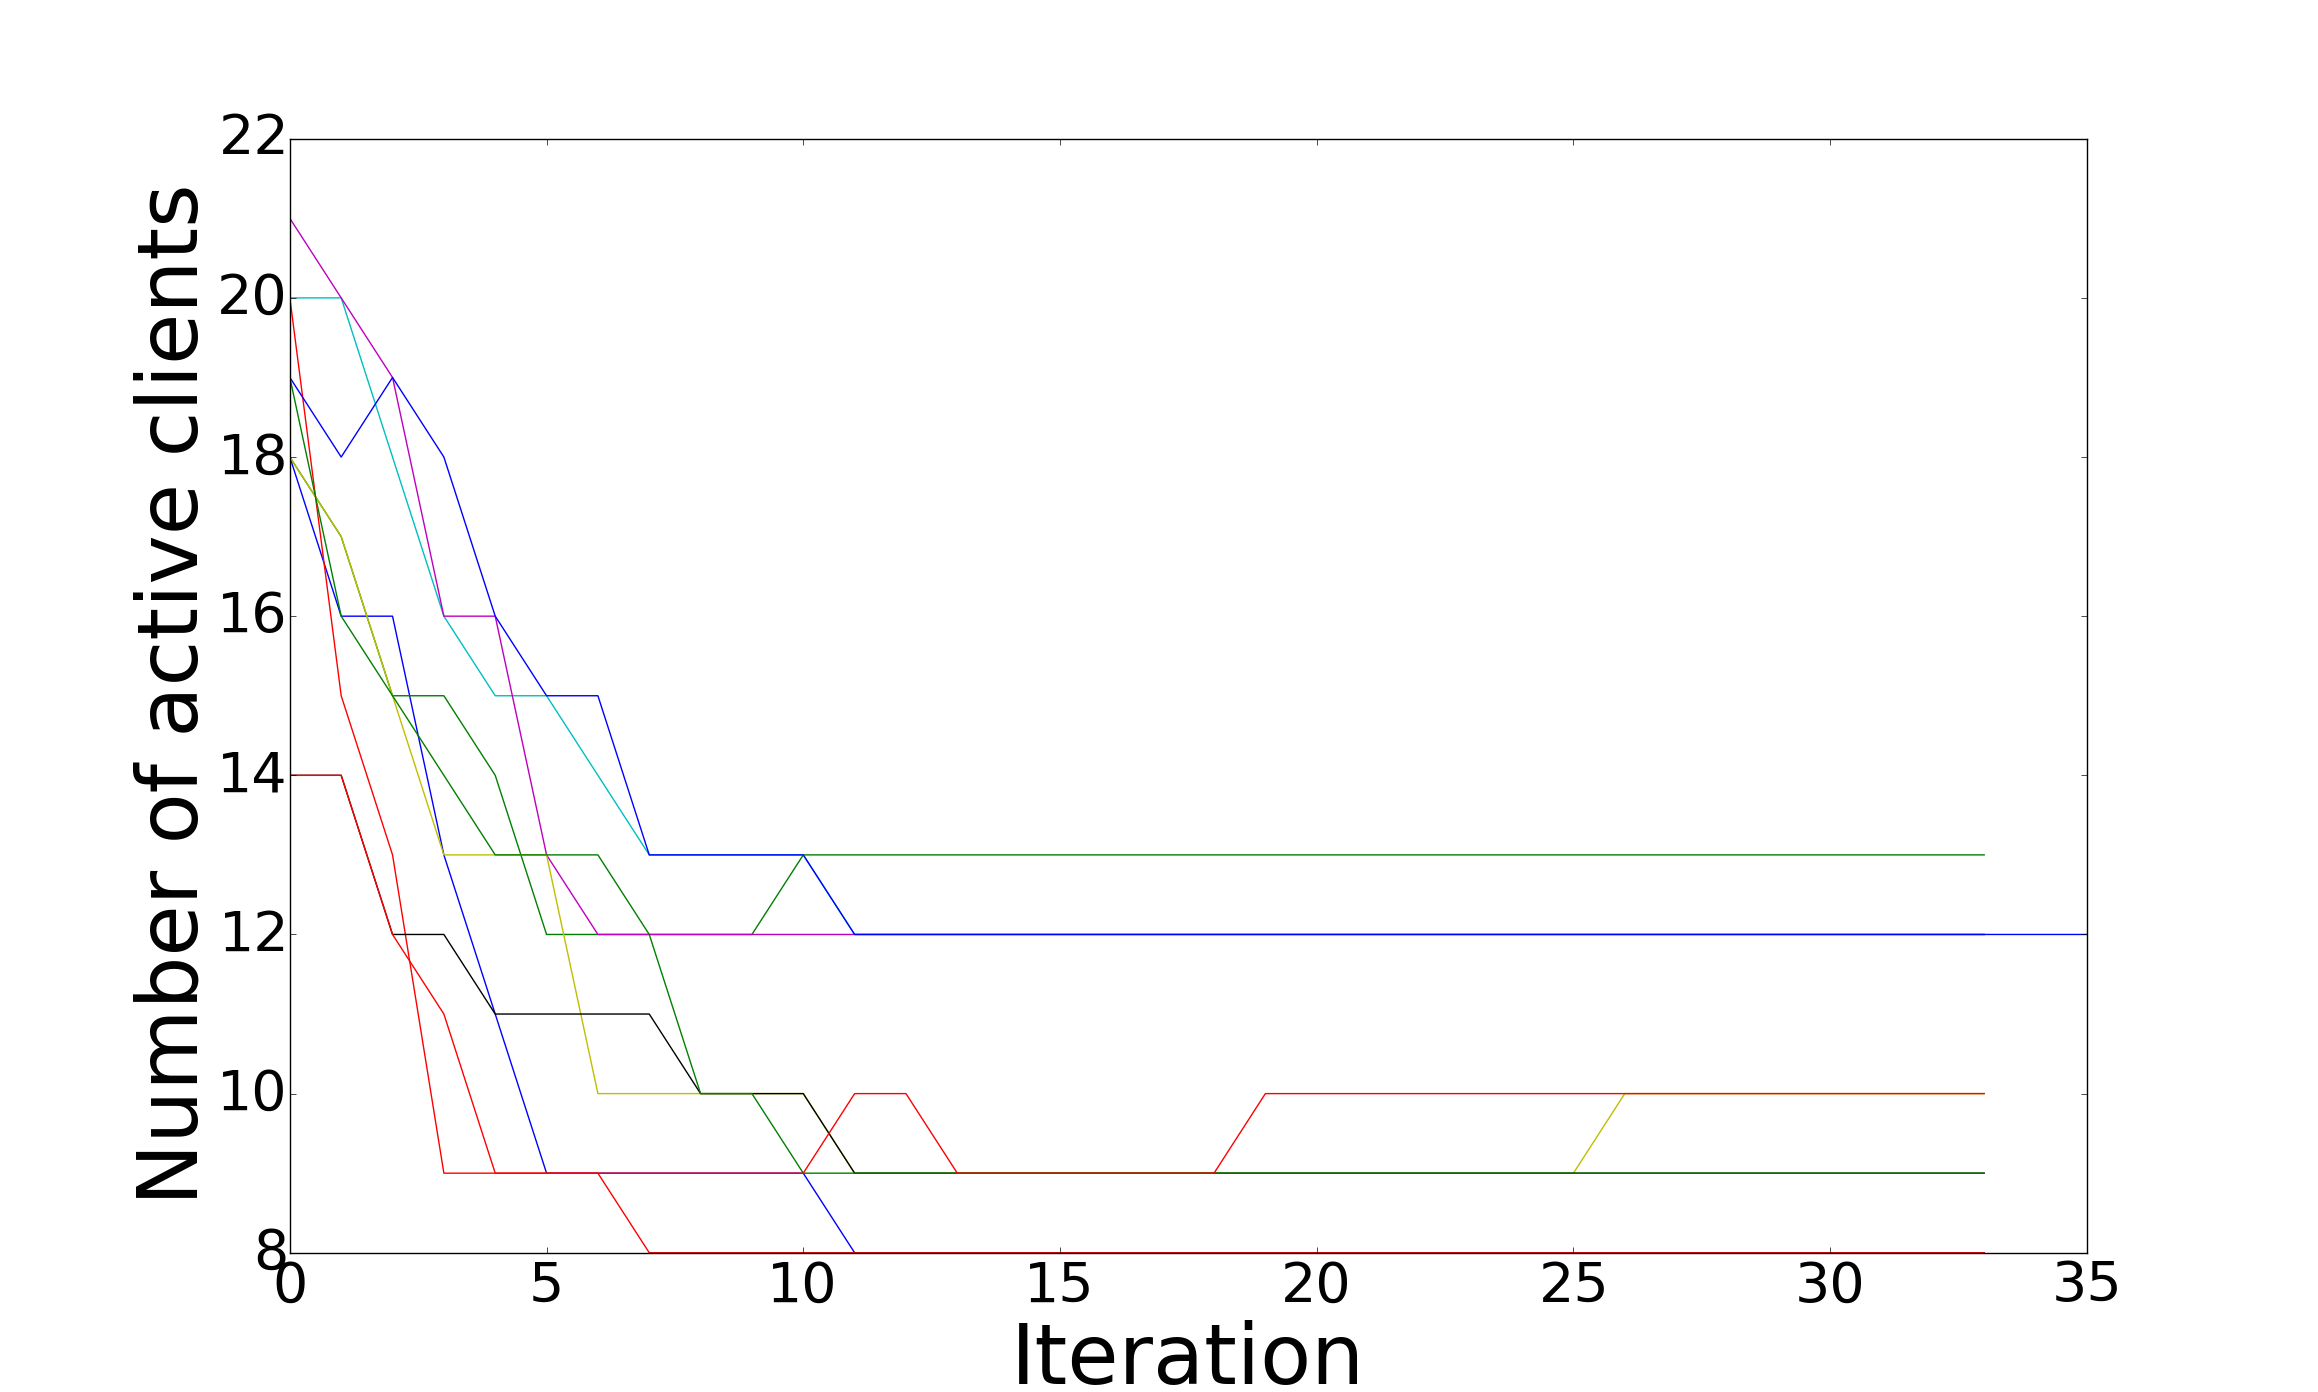
\includegraphics[width=\textwidth]{figures/v_iteration_logreg}
        \caption{Reduction of annotator subset}

    \end{subfigure}
    \caption{Training process}
    \label{fig:optimization}
\end{figure}




\subsection{Performance per task}

In the following figures we examine the breakdown of classification error rate per labeling task. We can notice on \autoref{fig:pertask} that the performance of our classifier ensemble has a high variation, both when using a neural network and logistic regression.

\begin{figure}[!htb]
    \centering
    \begin{subfigure}[b]{0.45\textwidth}
        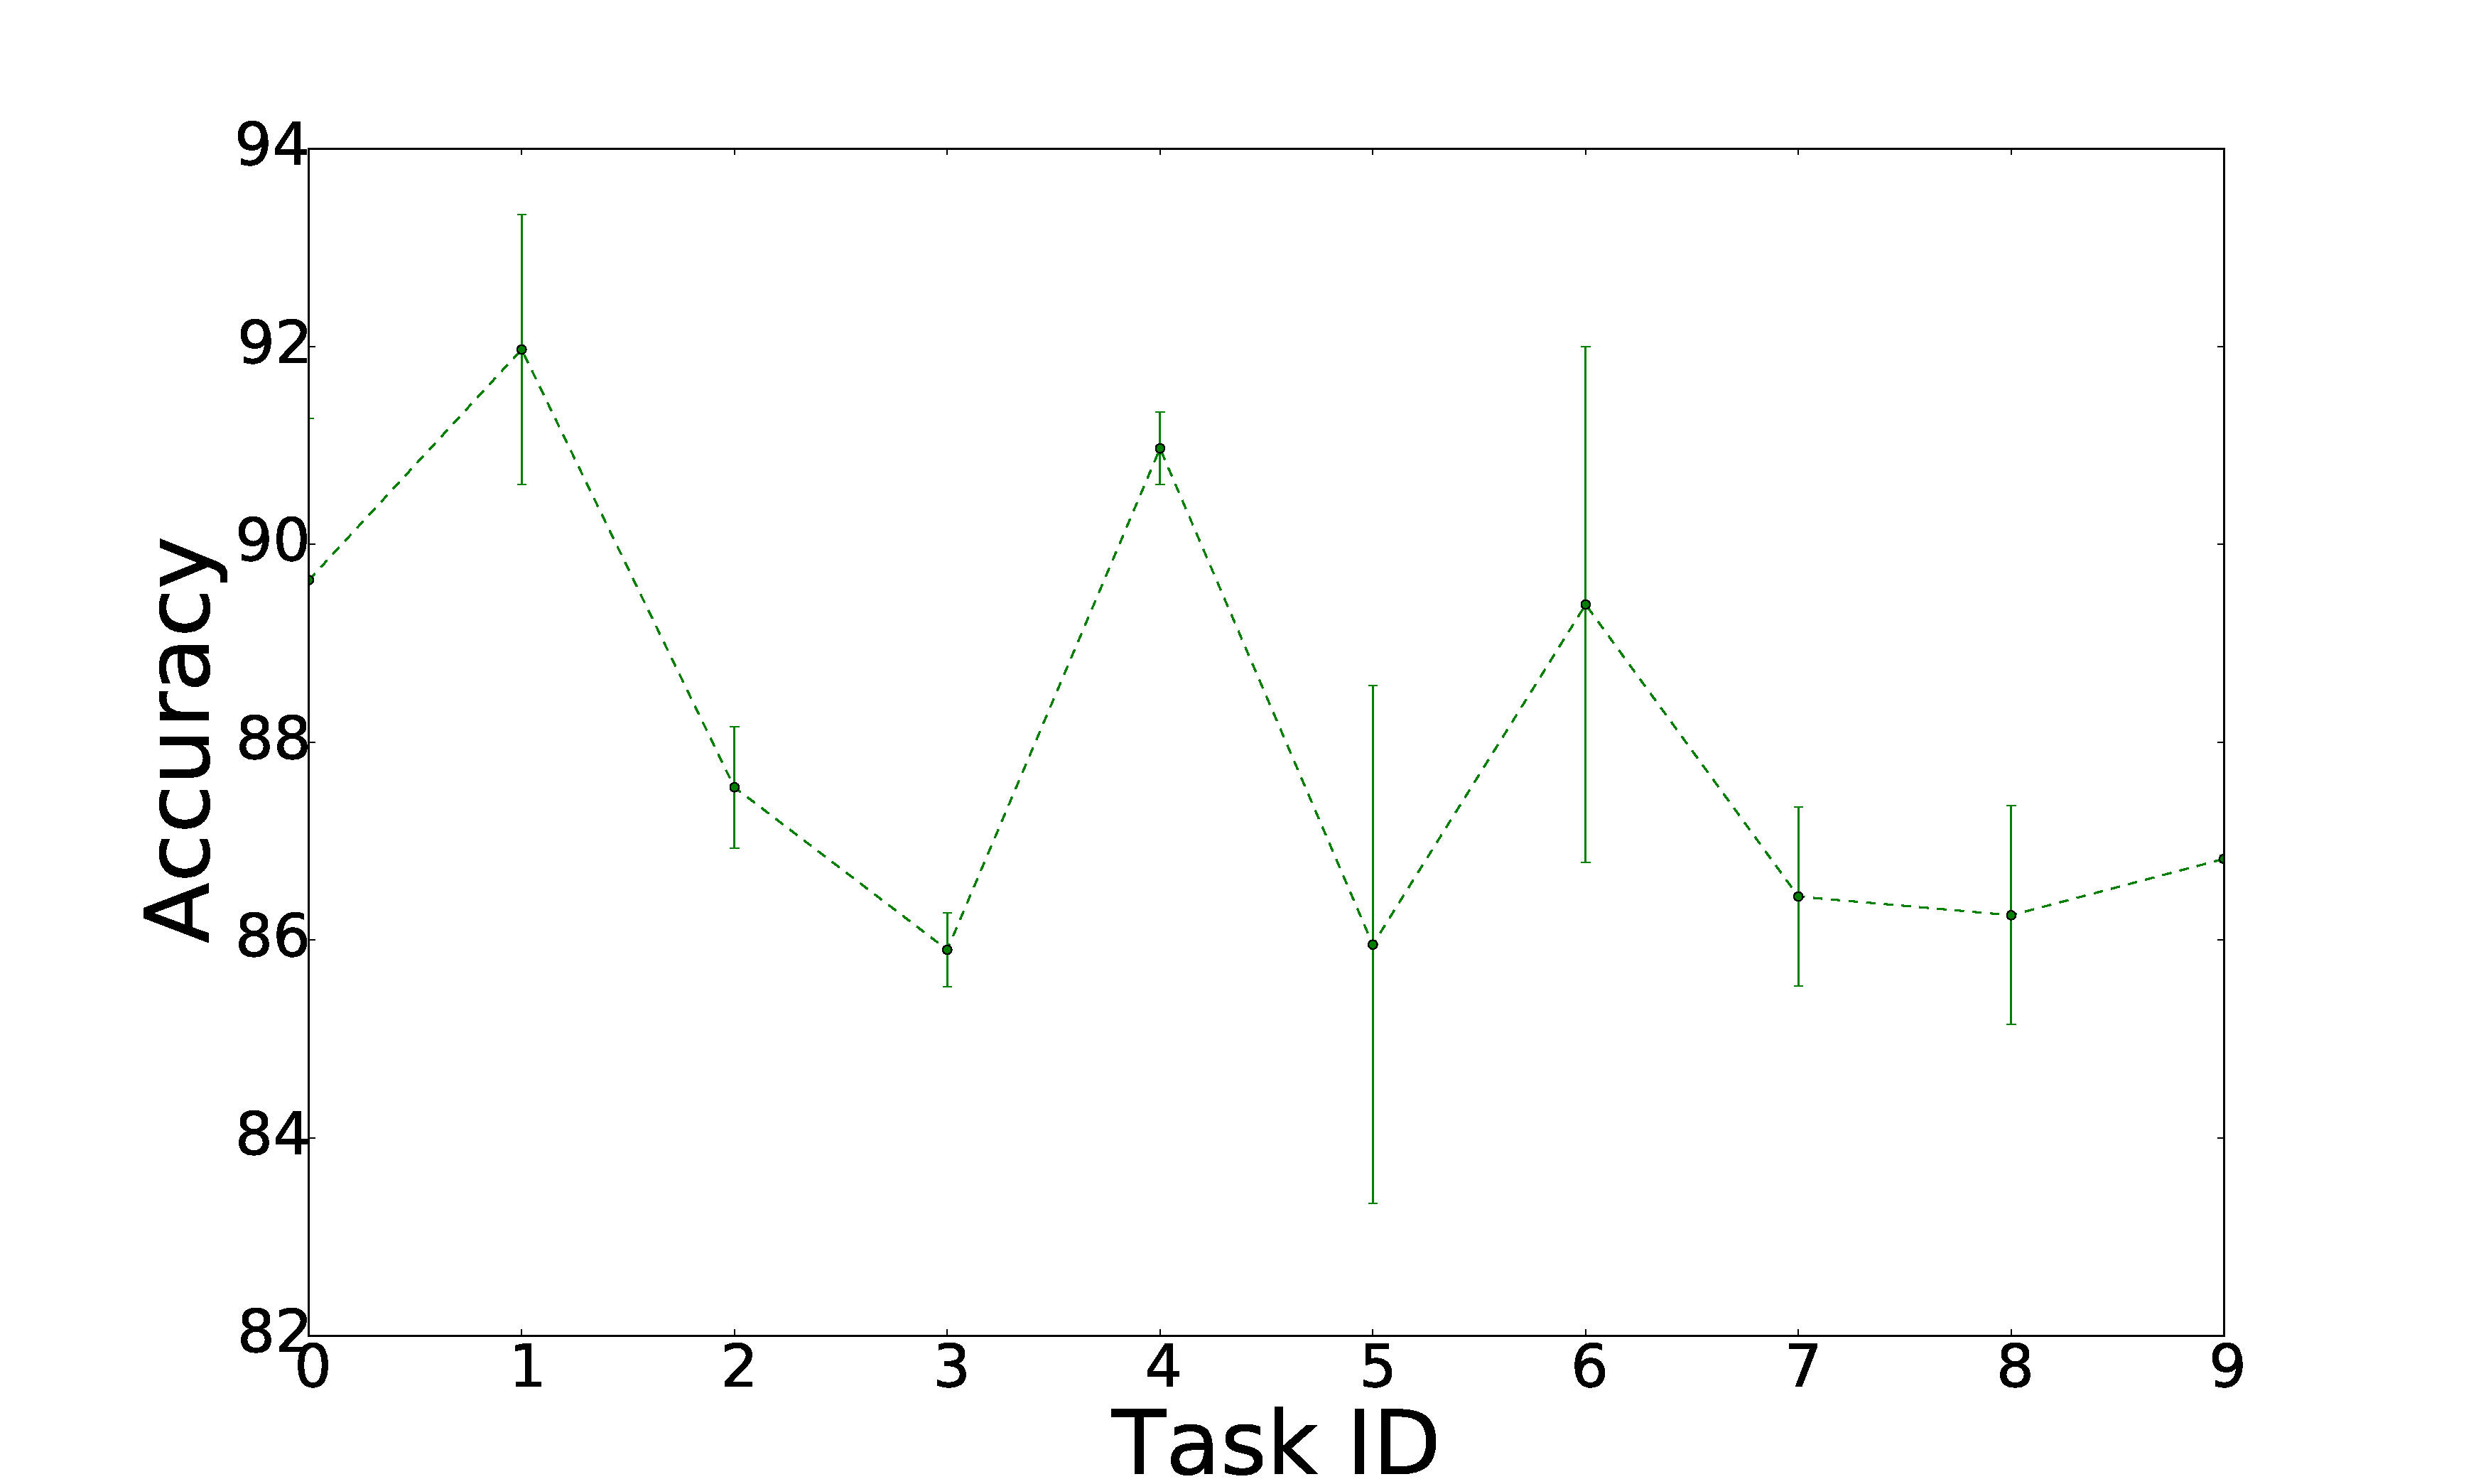
\includegraphics[width=\textwidth]{figures/task_logreg}
        \caption{A gull}
    \end{subfigure}
    \begin{subfigure}[b]{0.45\textwidth}
        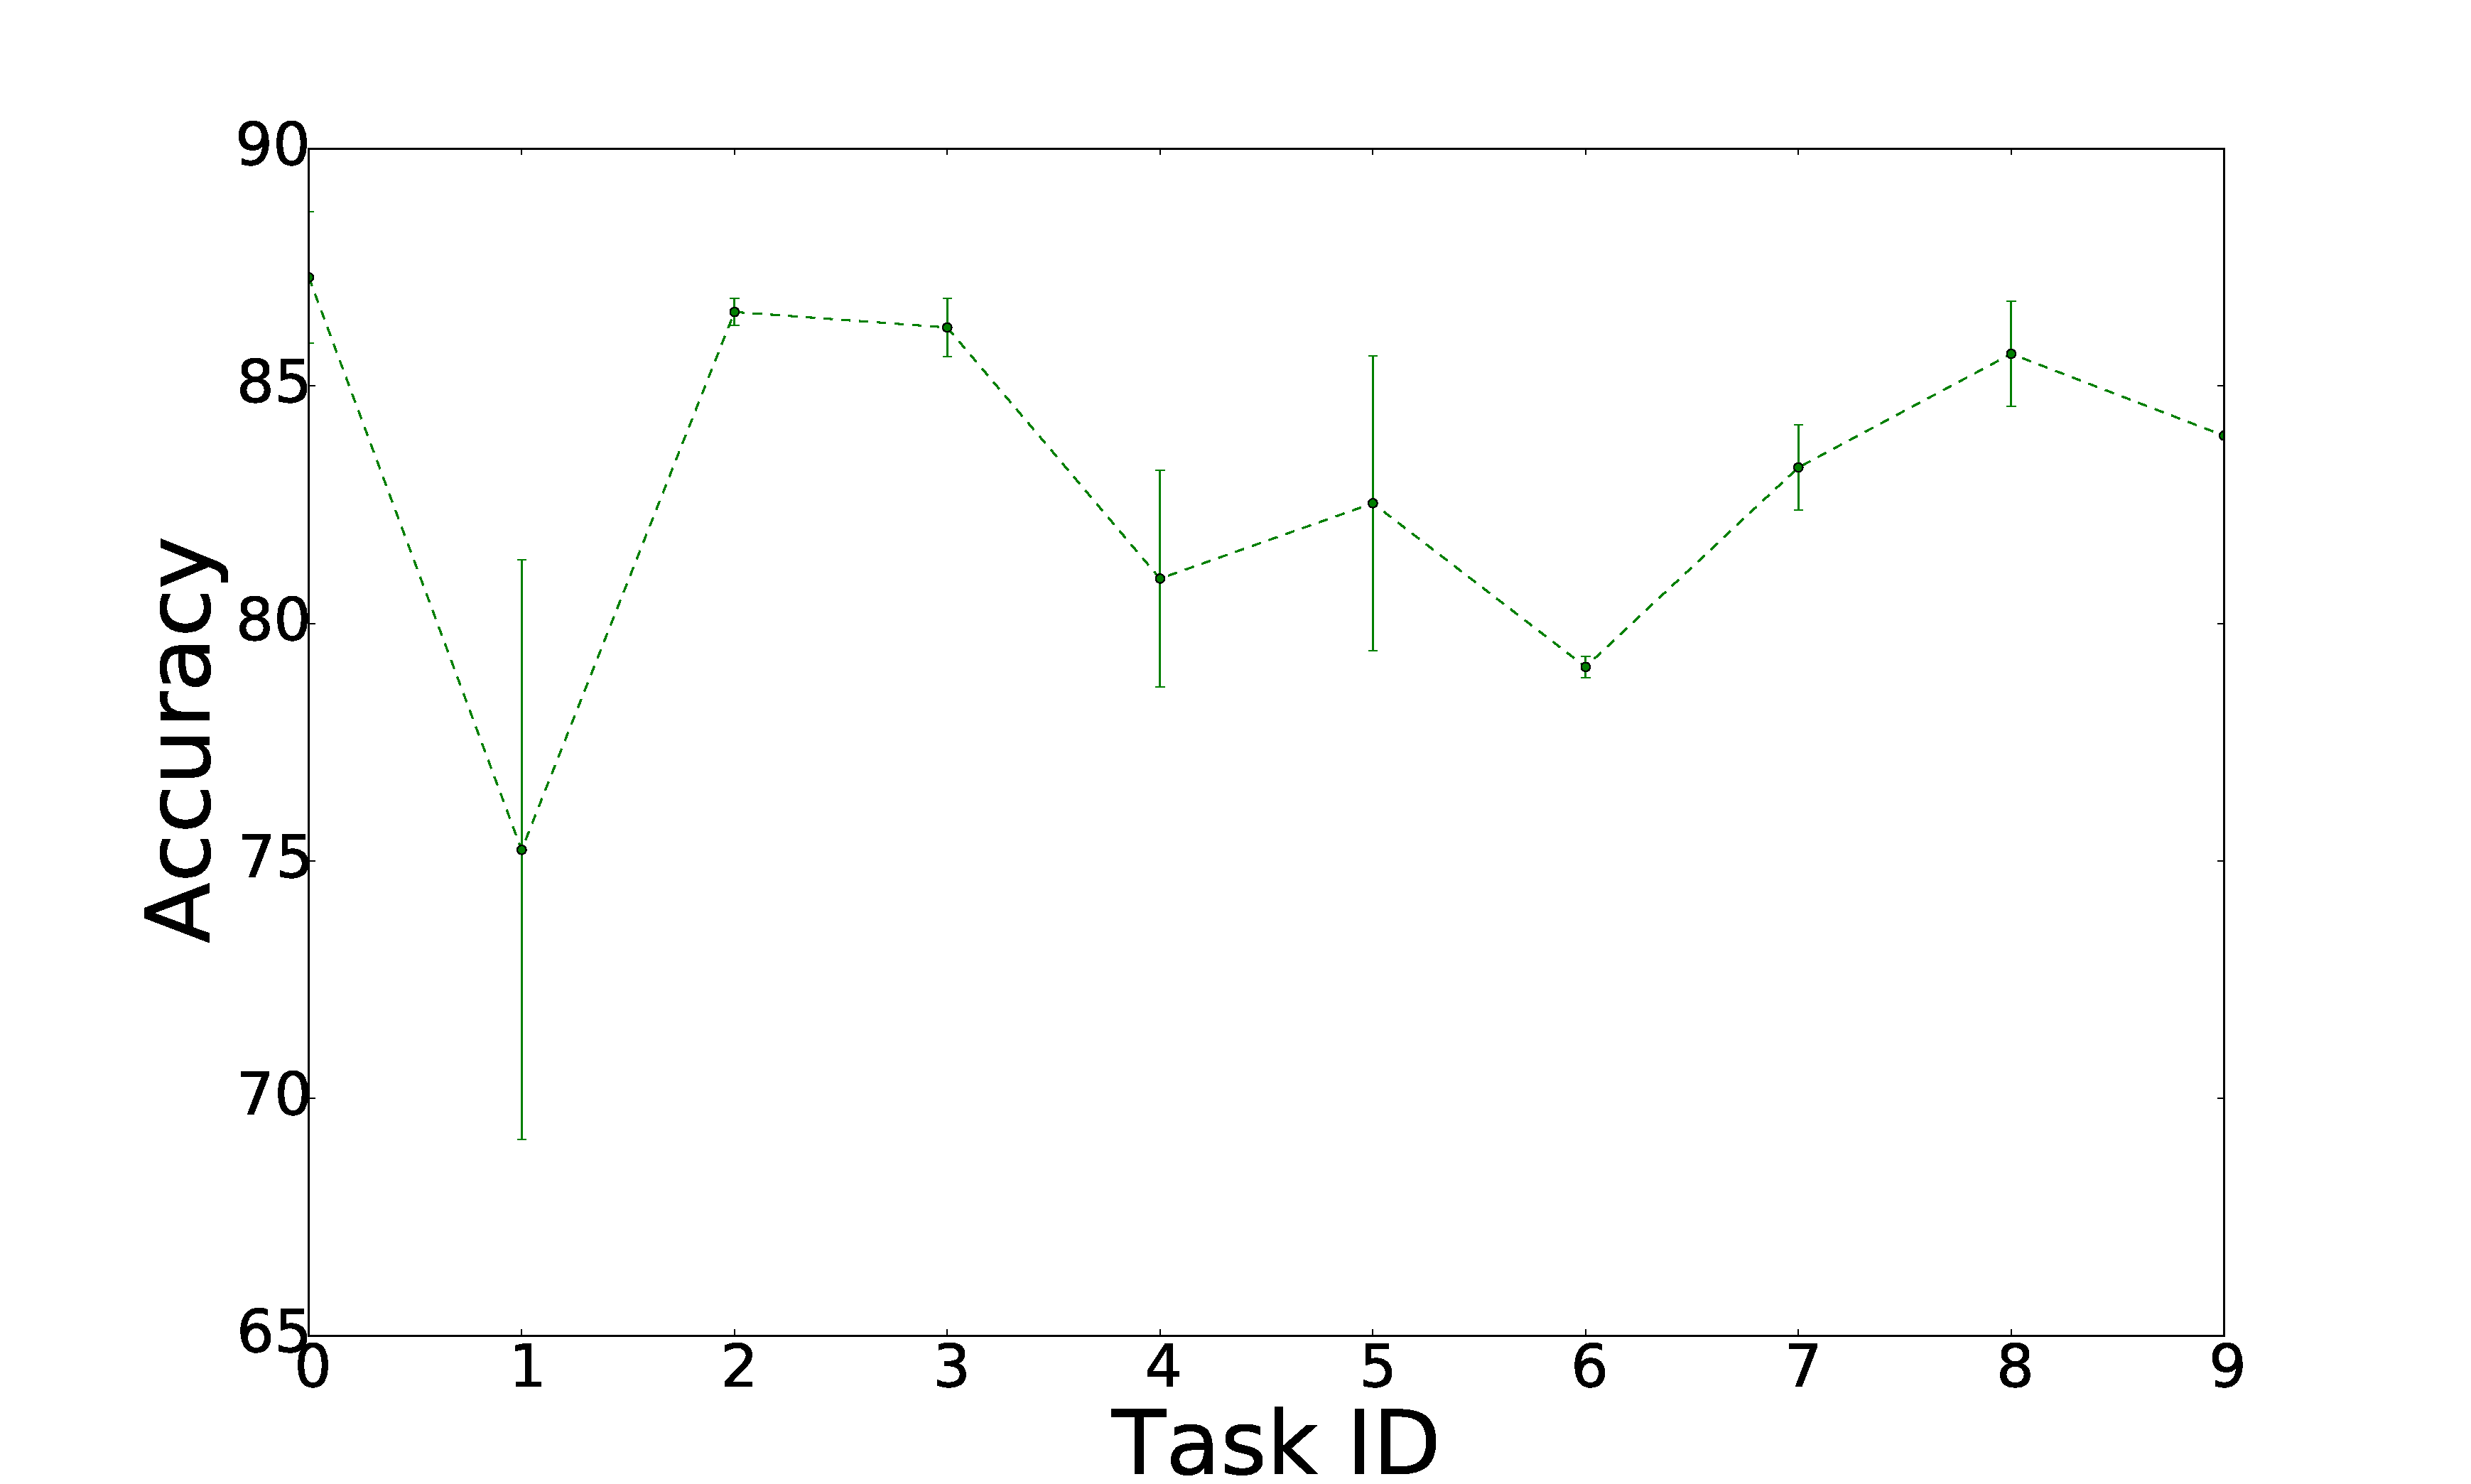
\includegraphics[width=\textwidth]{figures/task_mlp}
        \caption{A gull}
    \end{subfigure}
    \caption{Performance per task}
    \label{fig:pertask}
    
\end{figure}


\subsection{Comparison with baseline ensemble methods}

Furthermore, we compare the performance of our scheme with annotator selection to some baseline ensemble methods, such as averaging annotator values and taking a majority vote. %Moreover, we also compare our performance with a system that randomly chooses annotators. 
This comparison is shown on Figure~\ref{fig:baseline}.

\begin{figure}[!htb]
    \centering
    \begin{subfigure}[b]{0.45\textwidth}
        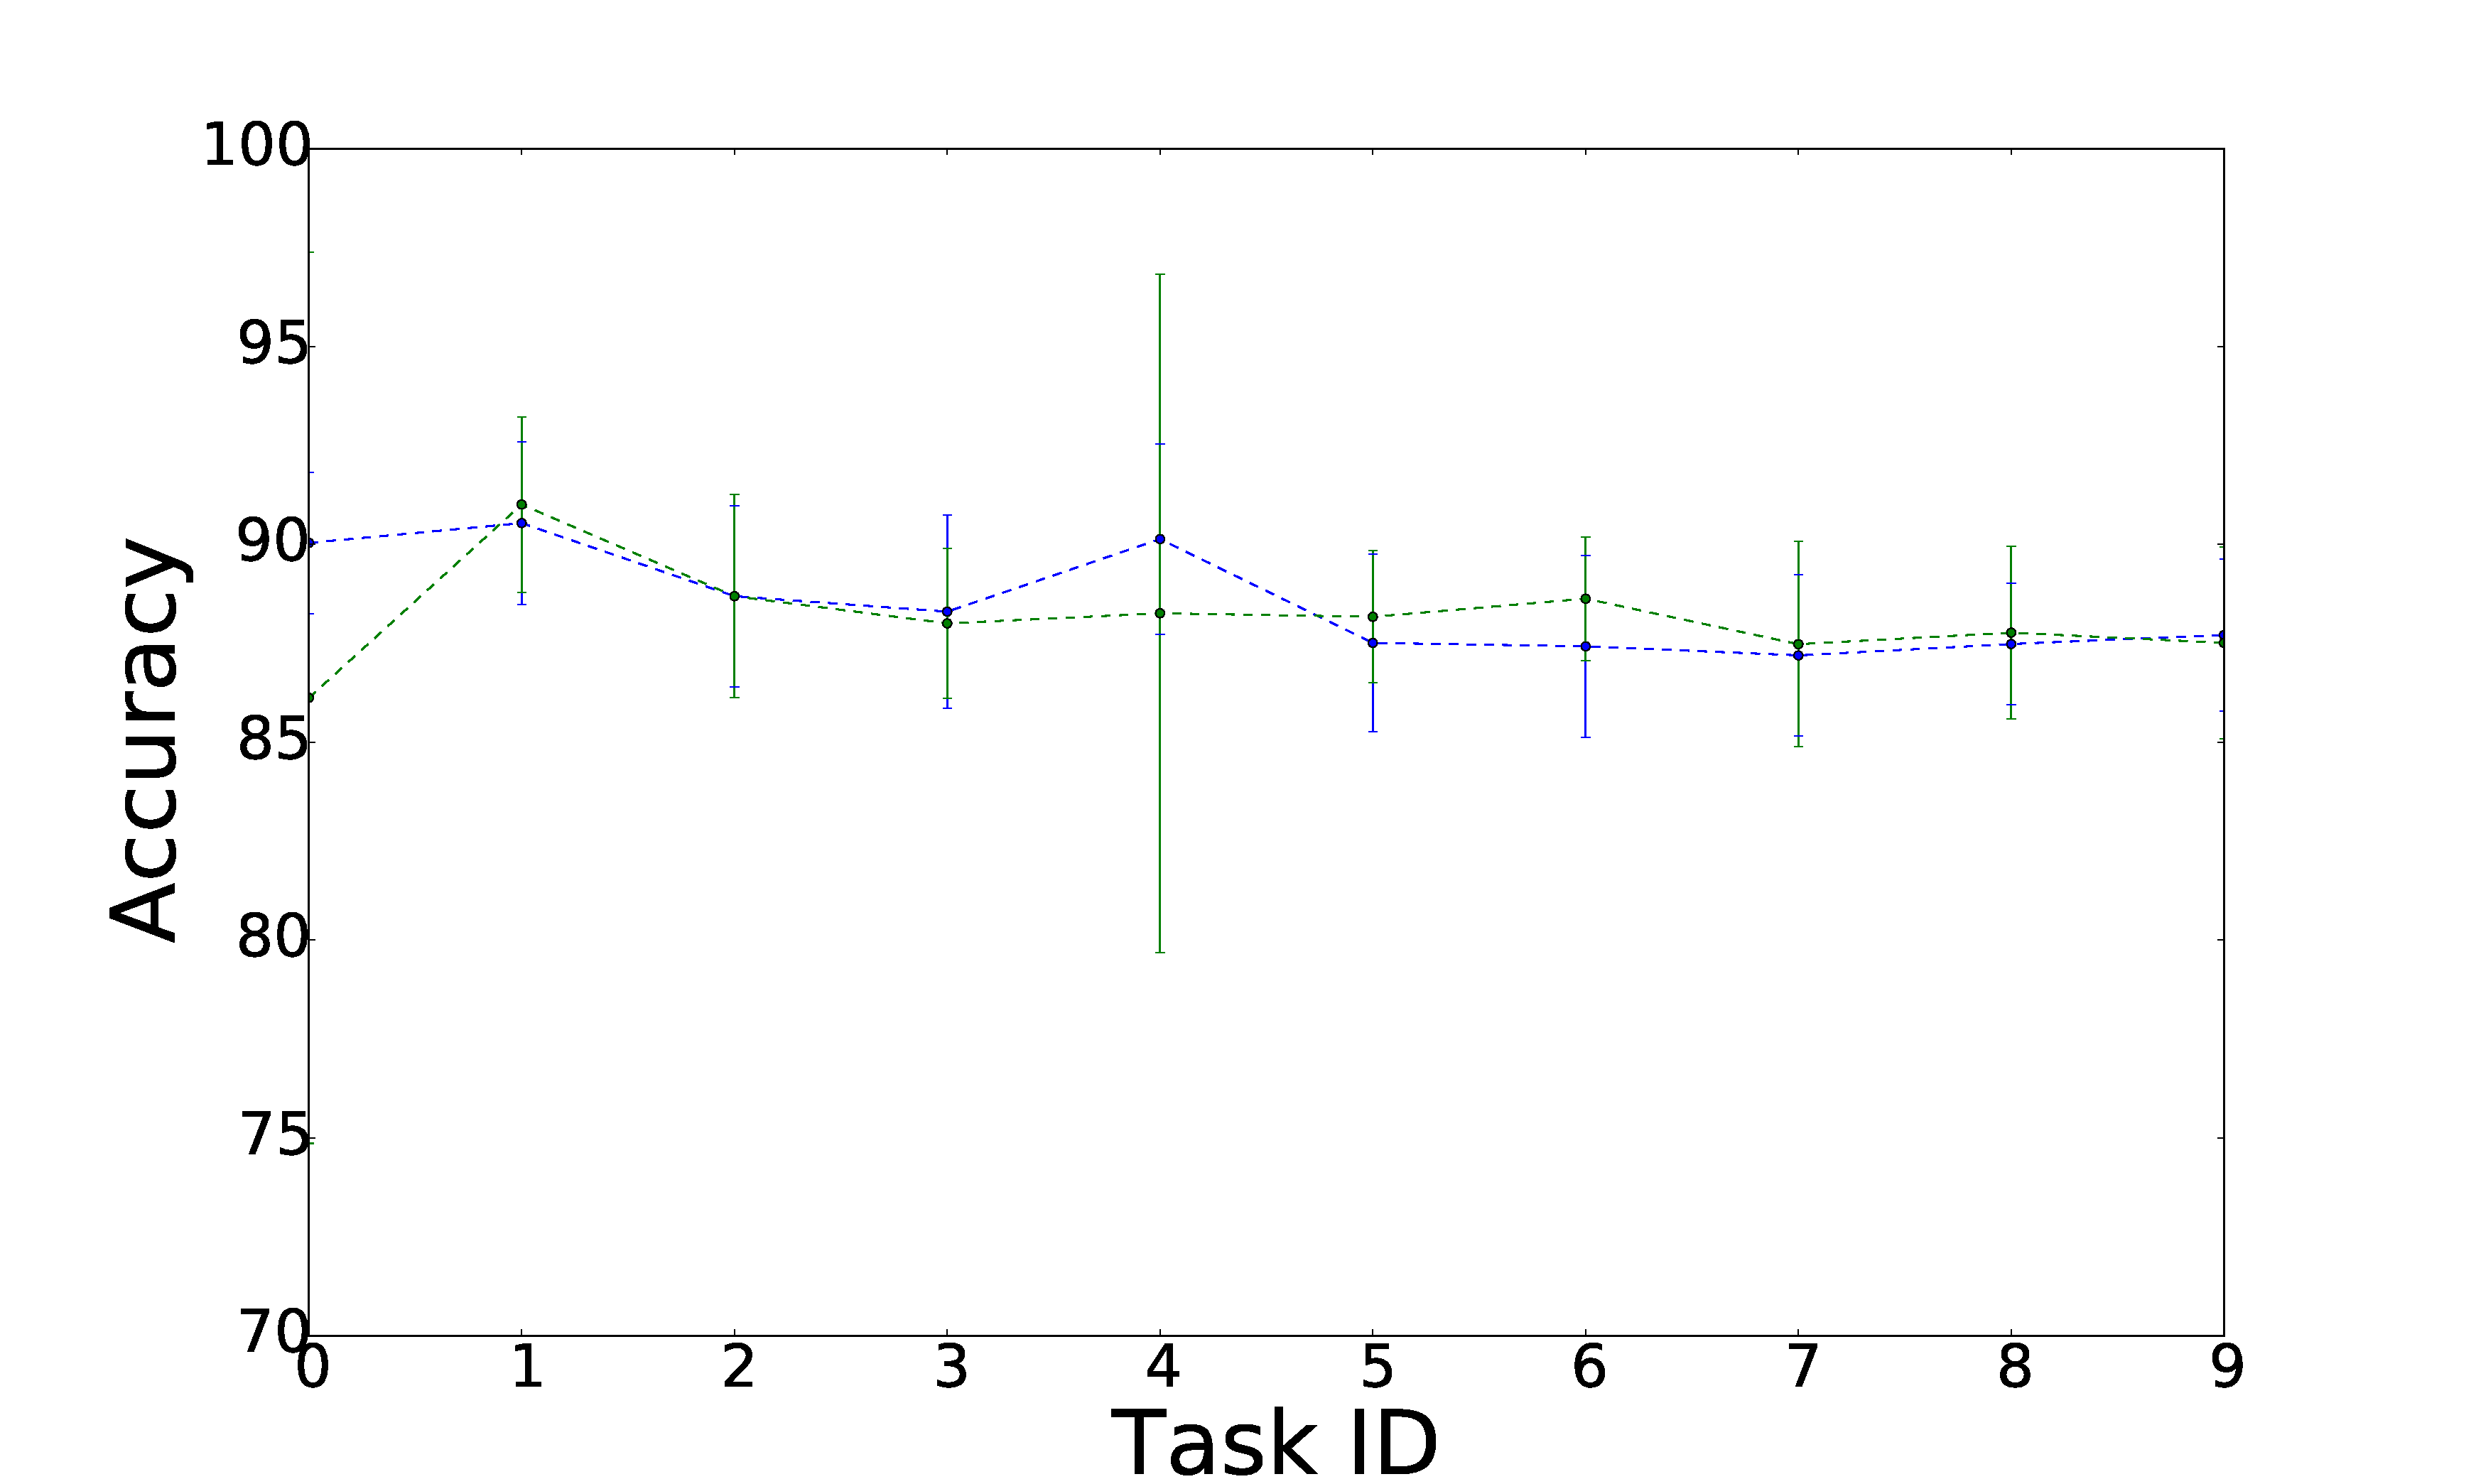
\includegraphics[width=\textwidth]{figures/comp_average}
        \caption{A gull}
    \end{subfigure}
    \begin{subfigure}[b]{0.45\textwidth}
        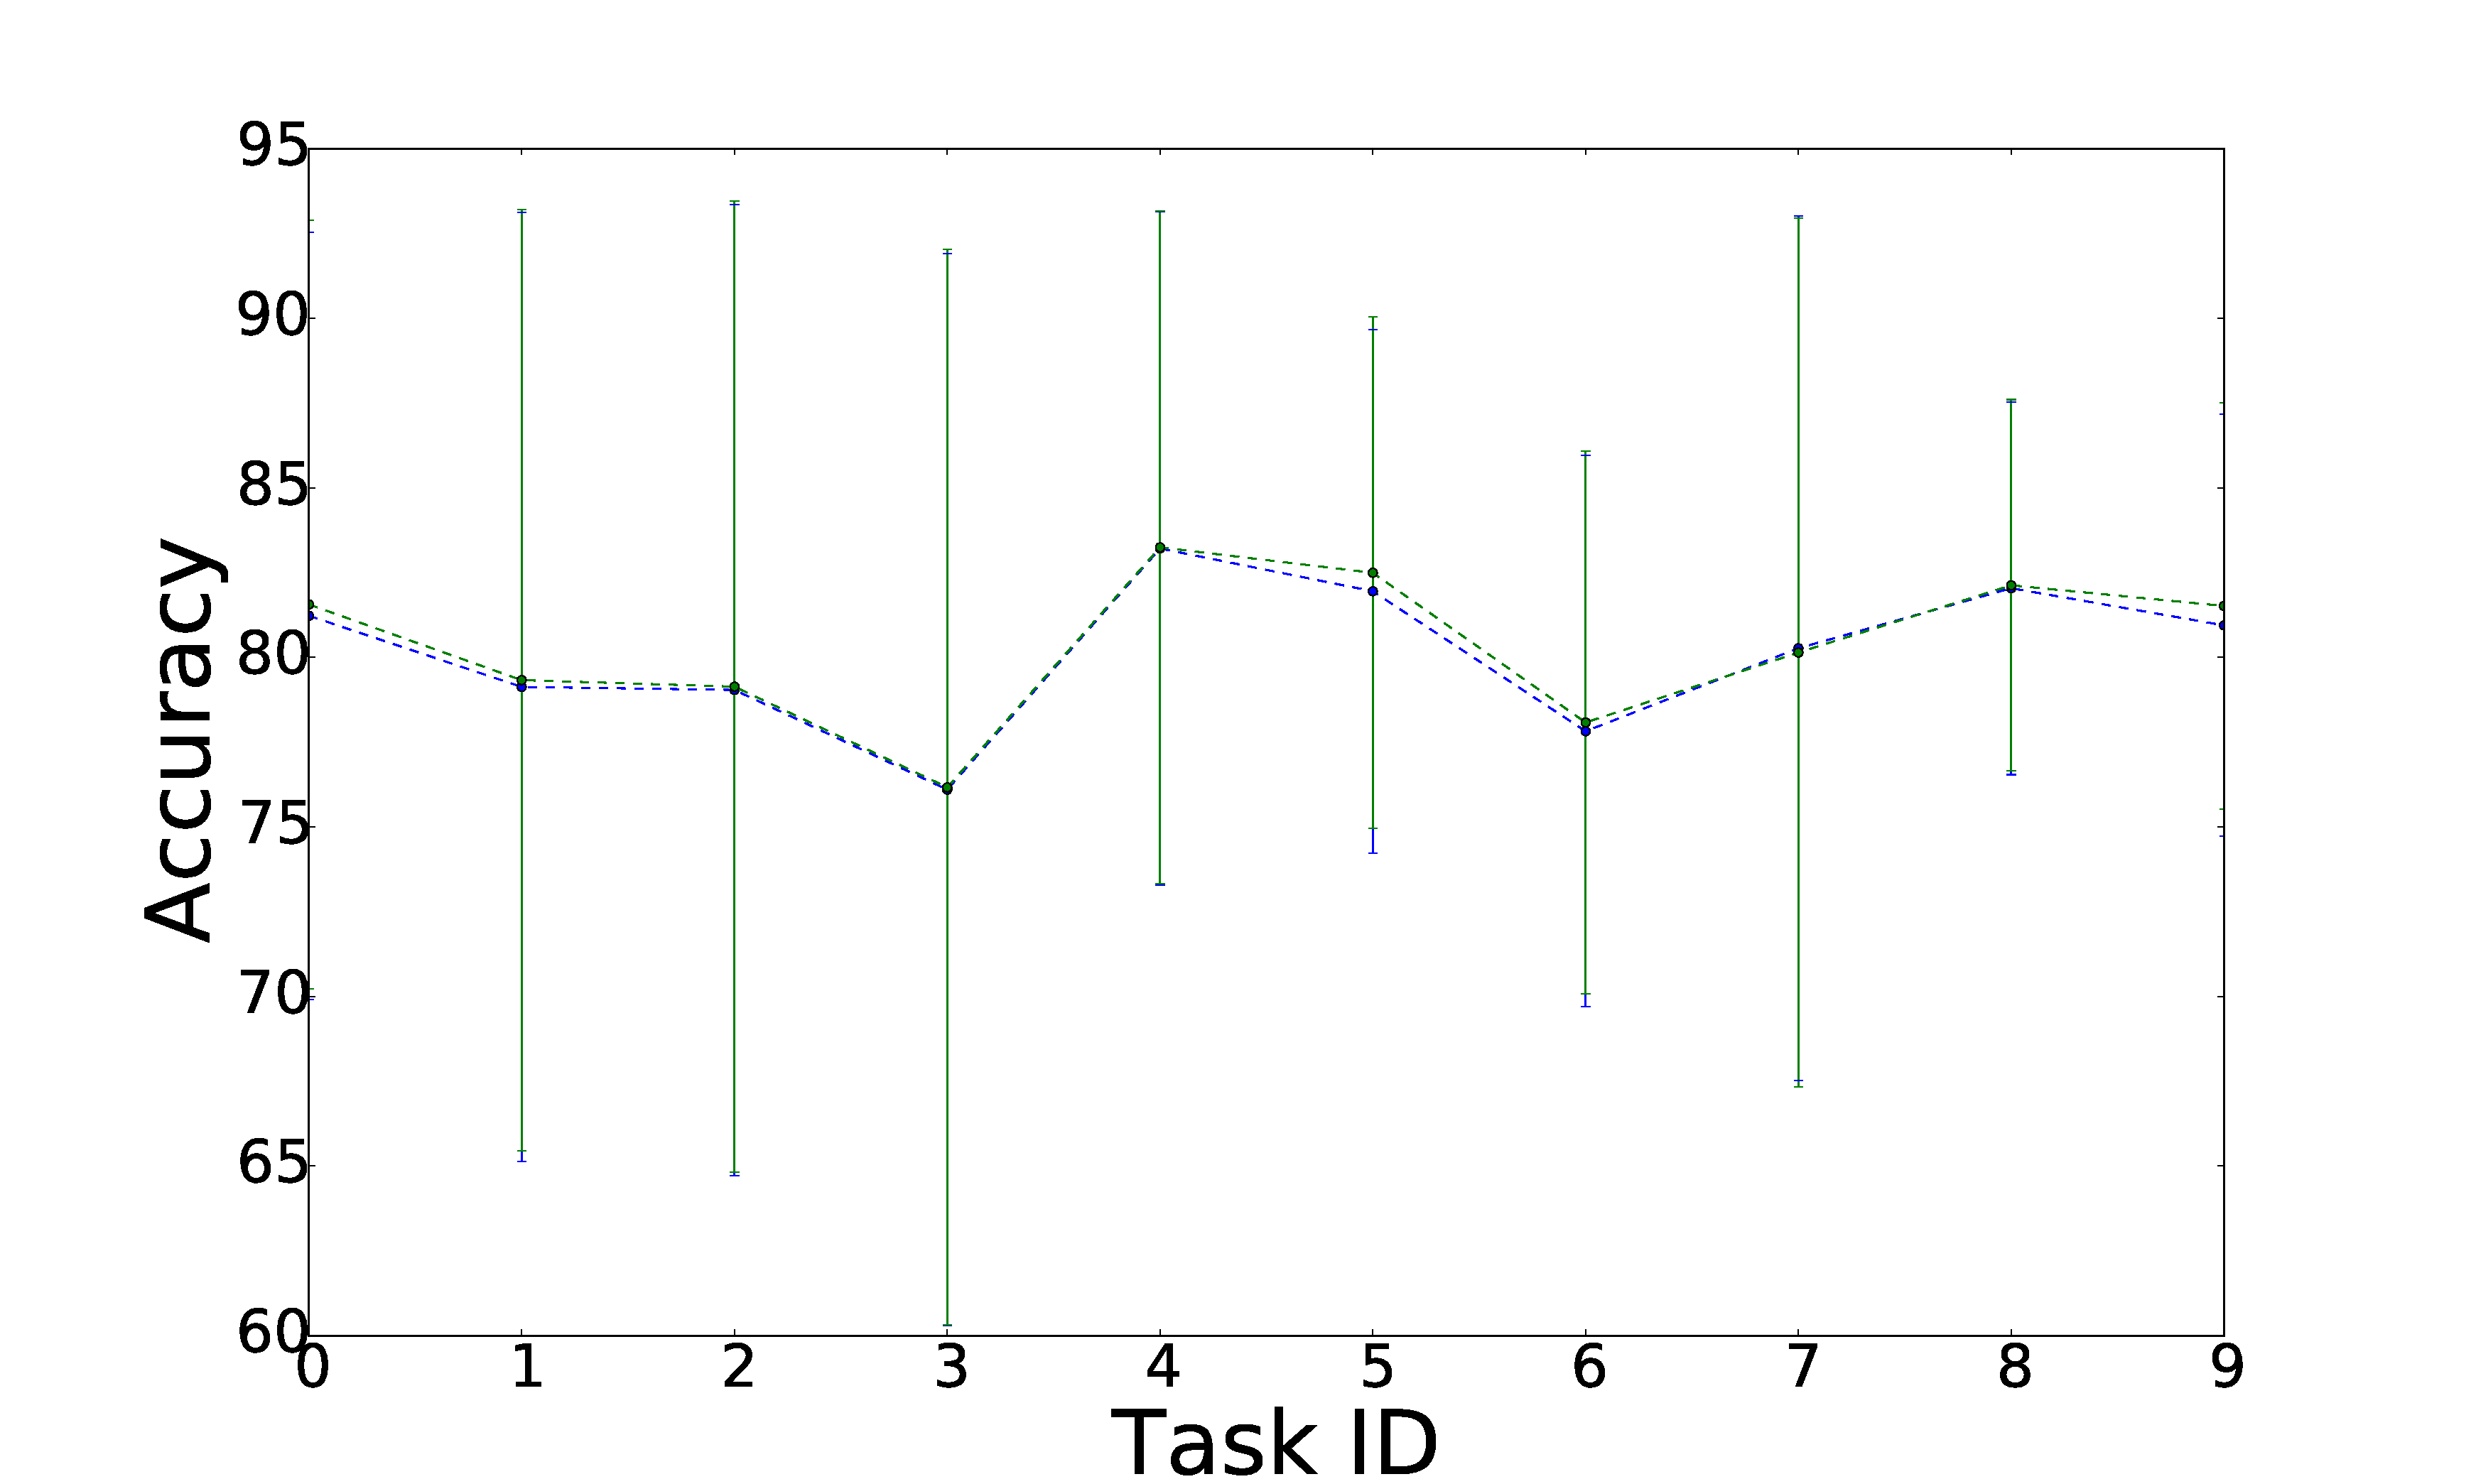
\includegraphics[width=\textwidth]{figures/comp_average_mlp}
        \caption{A gull}
    \end{subfigure}
    \caption{Comparison with baseline}
    \label{fig:baseline}
\end{figure}


\subsection{Comparison of sparse and dense weight vectors}

In this subsection we test the performance penalty of enforcing sparsity on the annotator weight vectors. We evaluate our assumption that a low number of high-quality annotators can together incur high performance. This turns out to be true, according to our results, shown on \autoref{fig:sparsity}.

\begin{figure}[!htb]
    \centering
    \begin{subfigure}[b]{0.45\textwidth}
        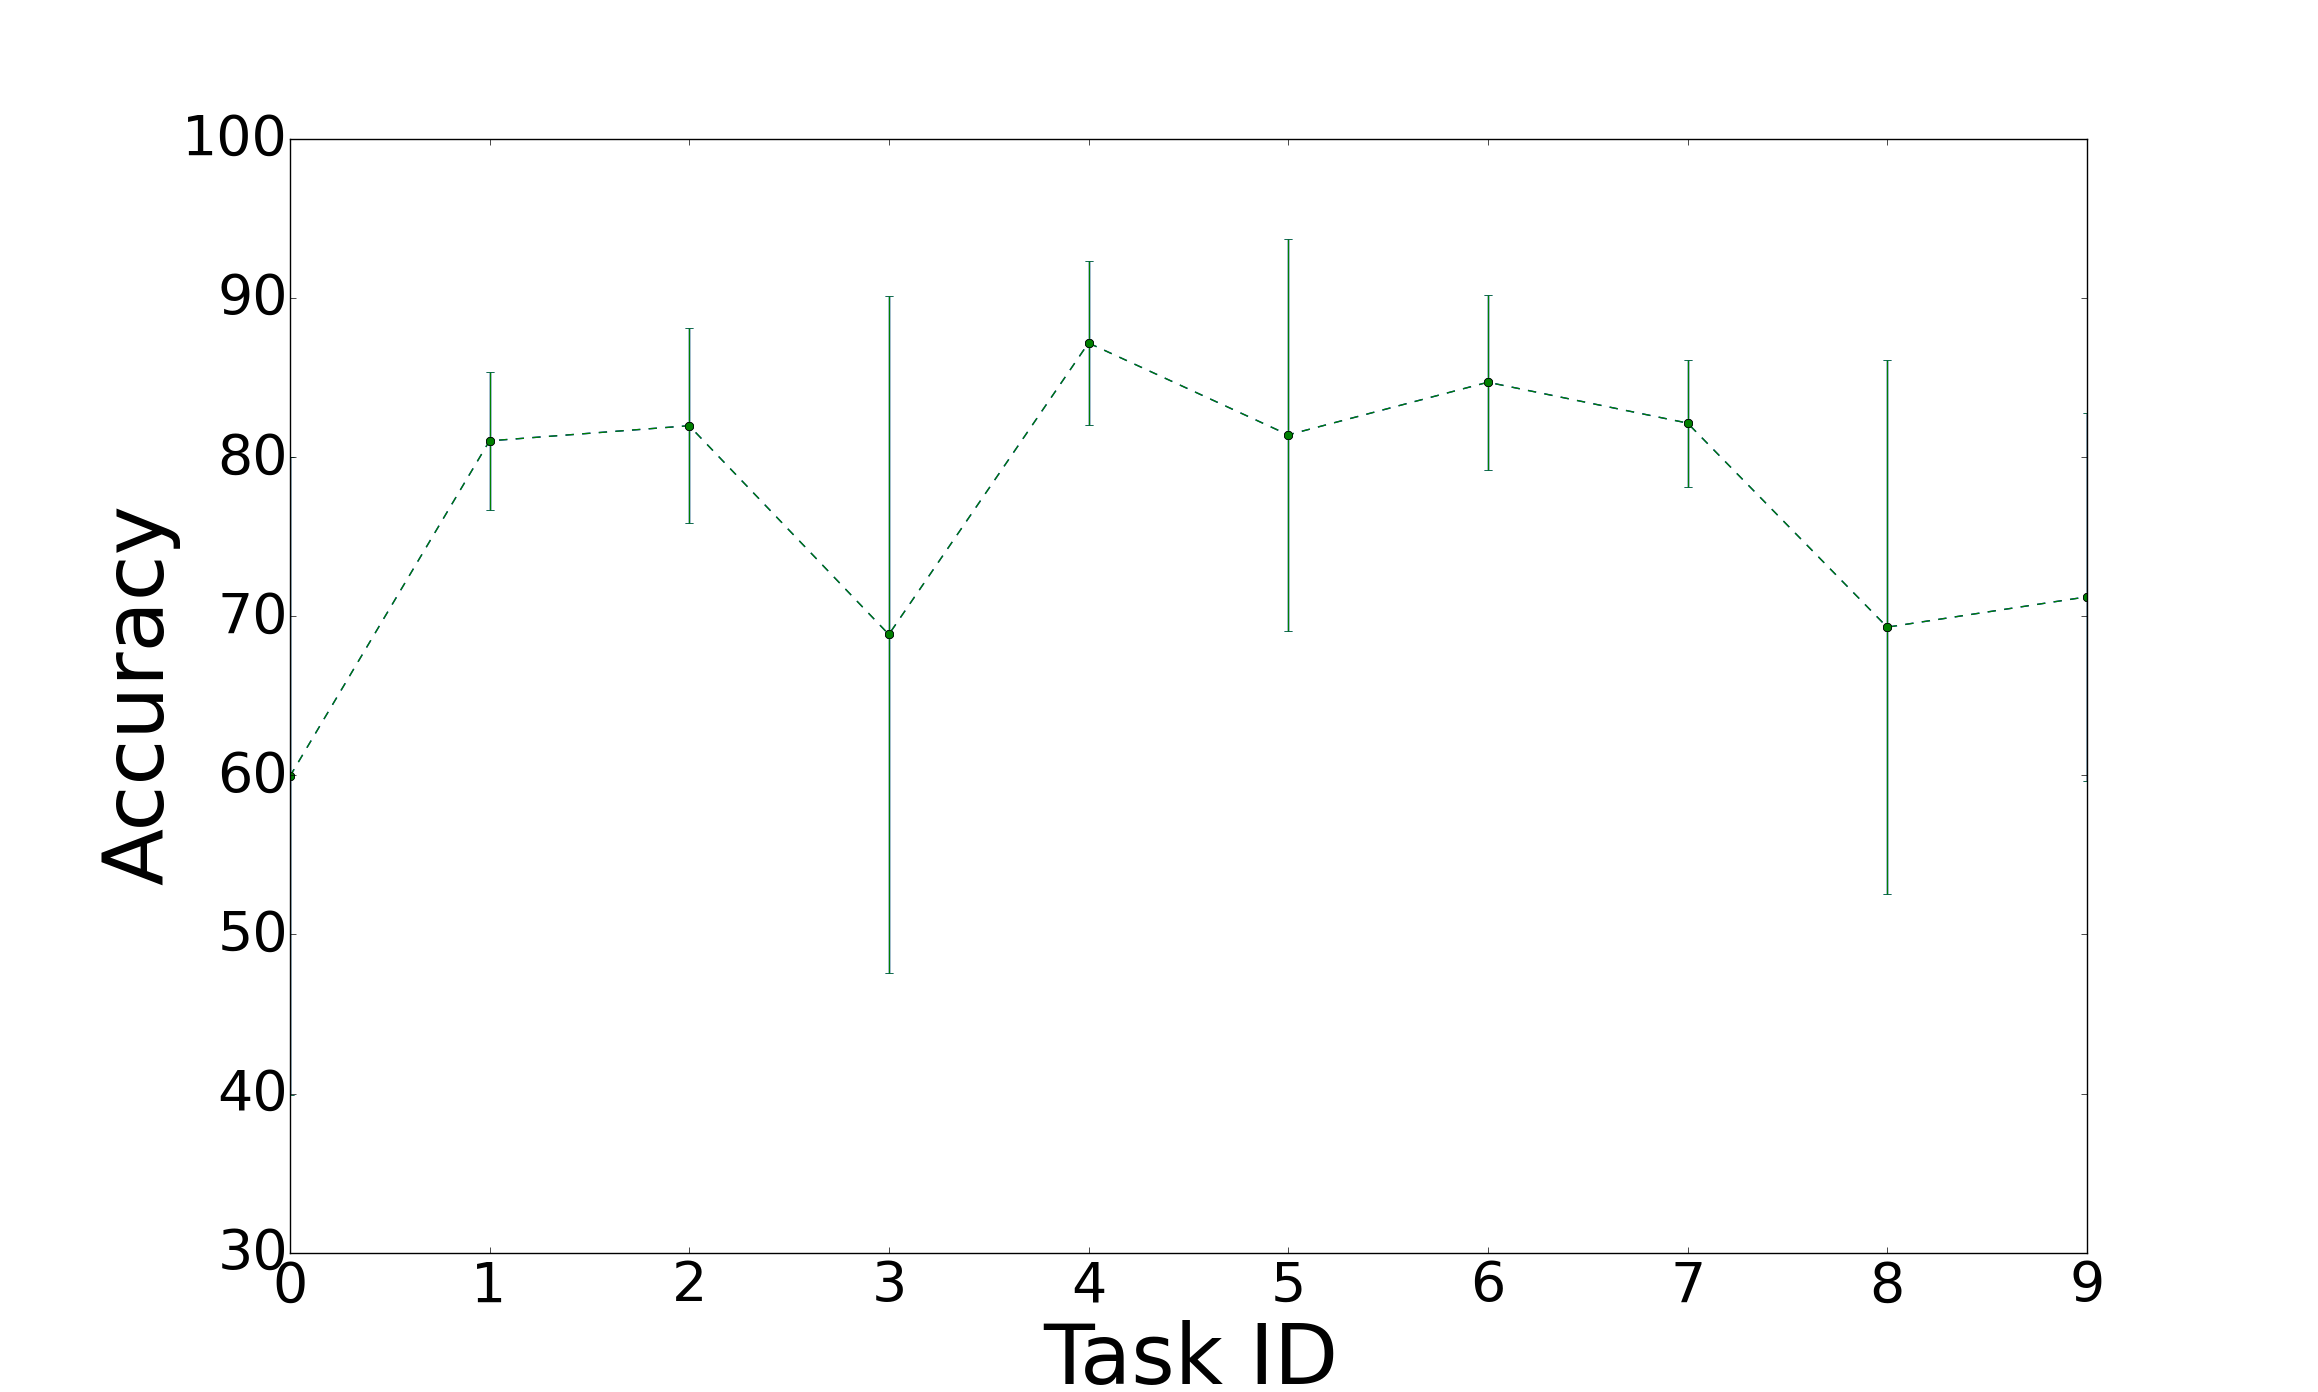
\includegraphics[width=\textwidth]{figures/plot_mlp}
        \caption{A gull}
    \end{subfigure}
    \begin{subfigure}[b]{0.45\textwidth}
        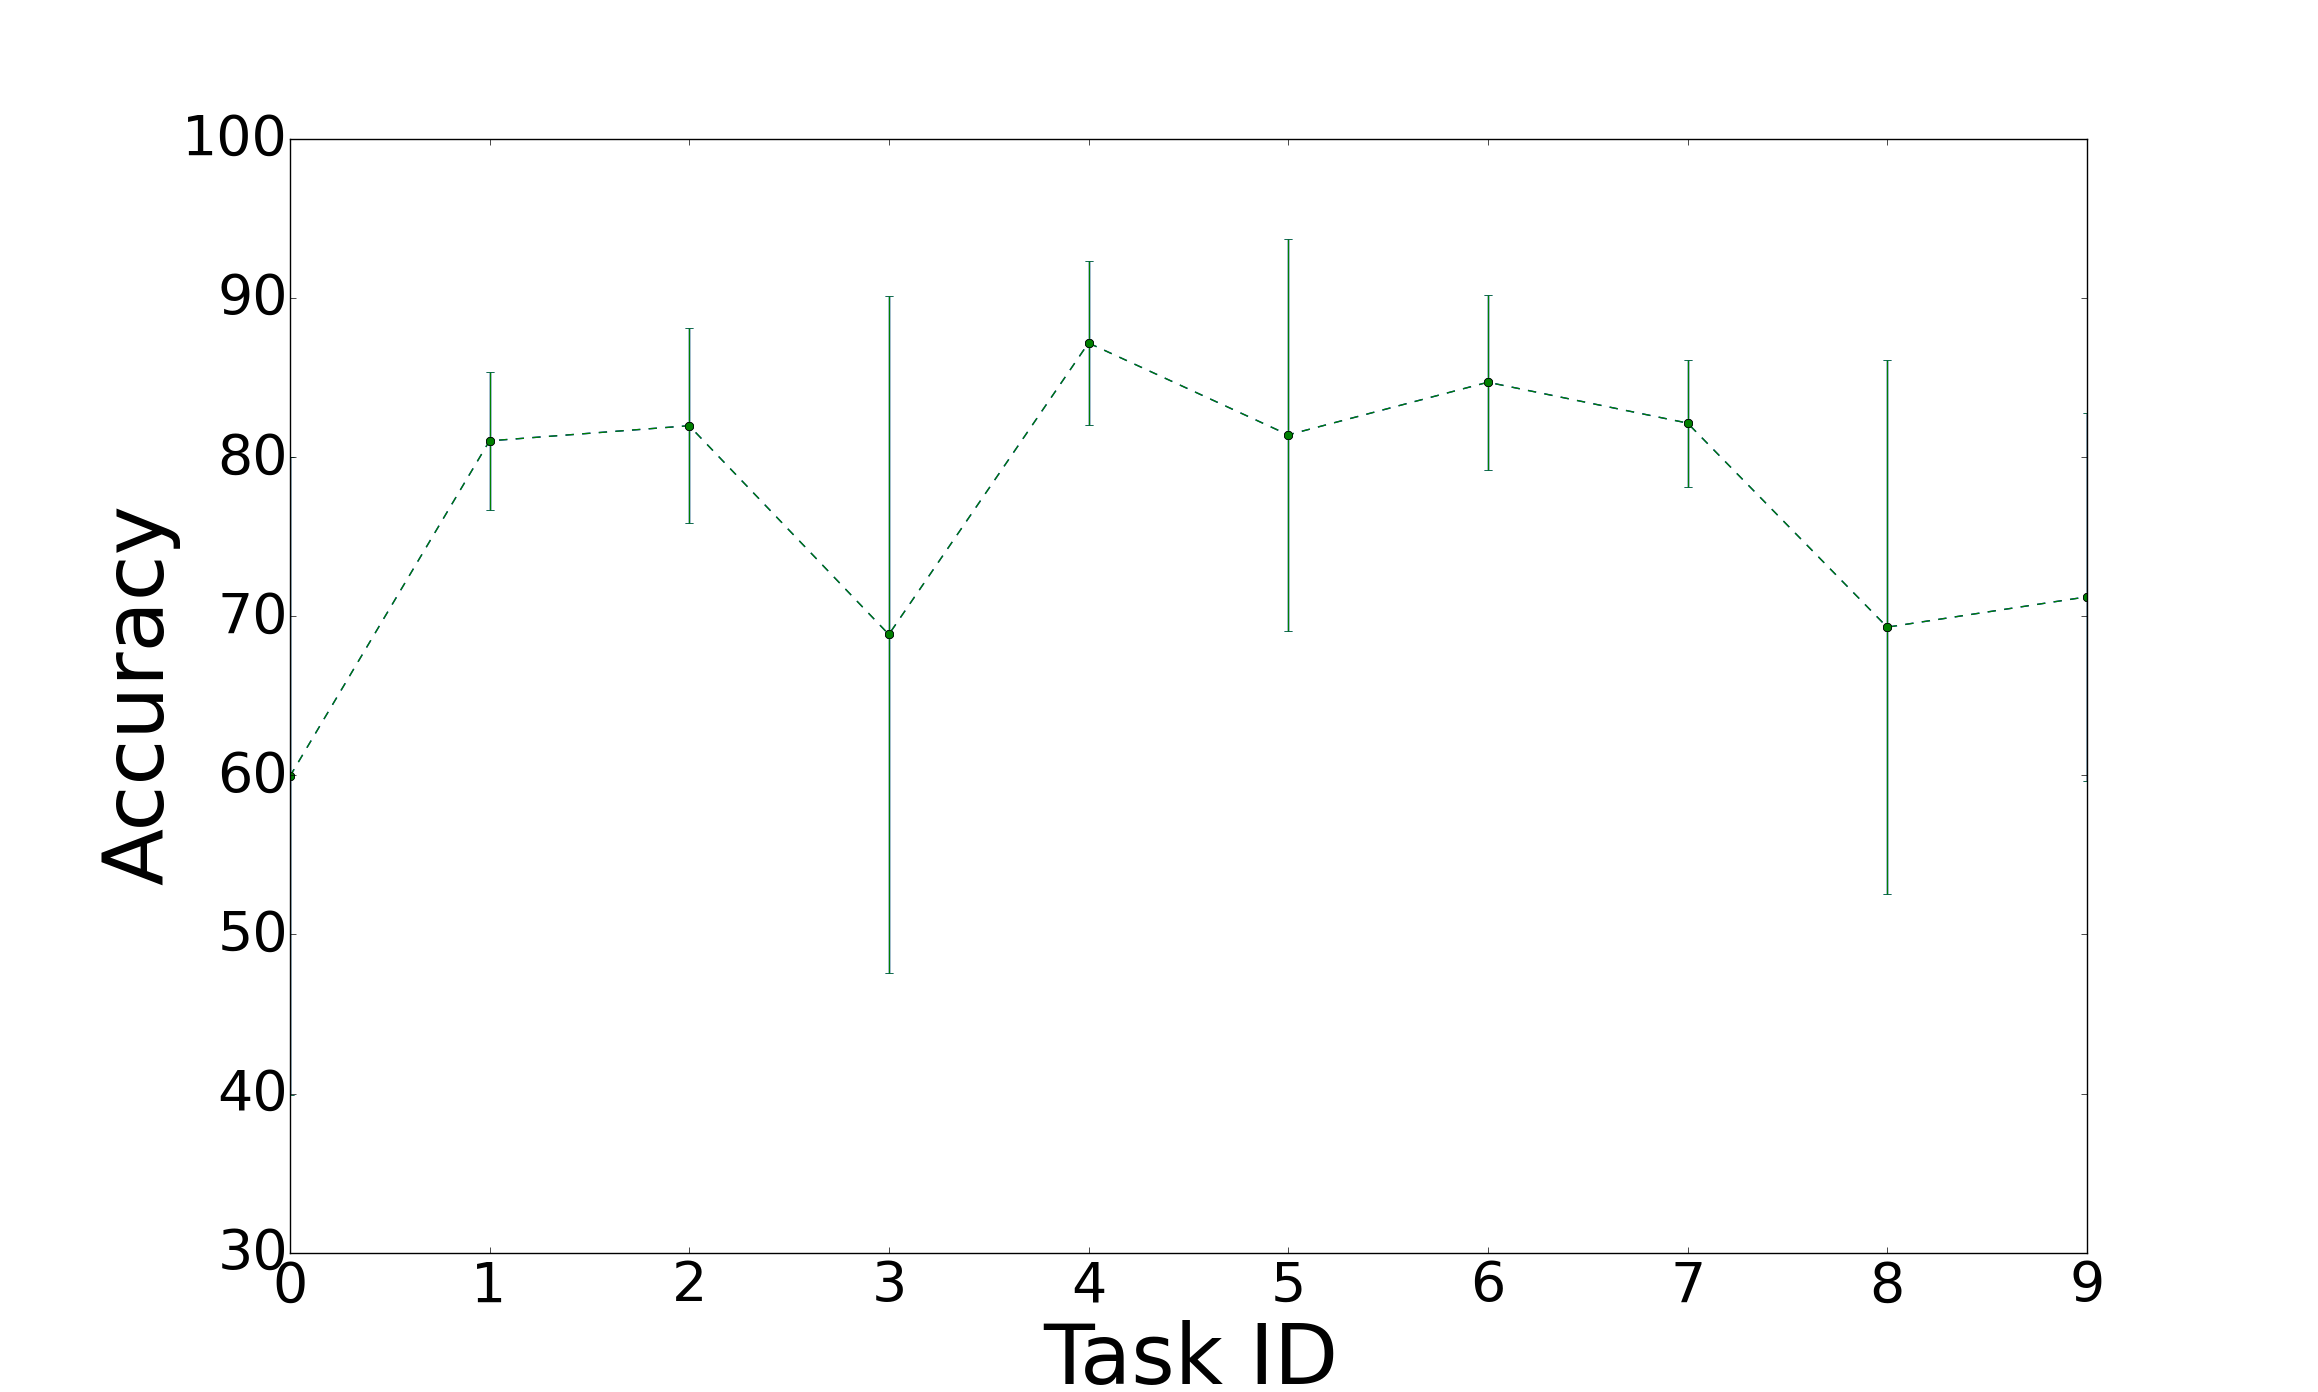
\includegraphics[width=\textwidth]{figures/plot_mlp}
        \caption{A gull}
    \end{subfigure}
    \caption{Effect of sparsity on model accuracy}
    \label{fig:sparsity}
\end{figure}


\subsection{Sensitivity to the weight of the regularization}

In the beginning, we examine the changes of the loss function when increasing the parameter $\lambda$ from 0 to 1, thereby adding the weight to the sparsity part of the loss function. The results of this test are displayed on \autoref{fig:sensitivity}.

\begin{figure}[!htb]
    \centering
    \begin{subfigure}[b]{0.45\textwidth}
        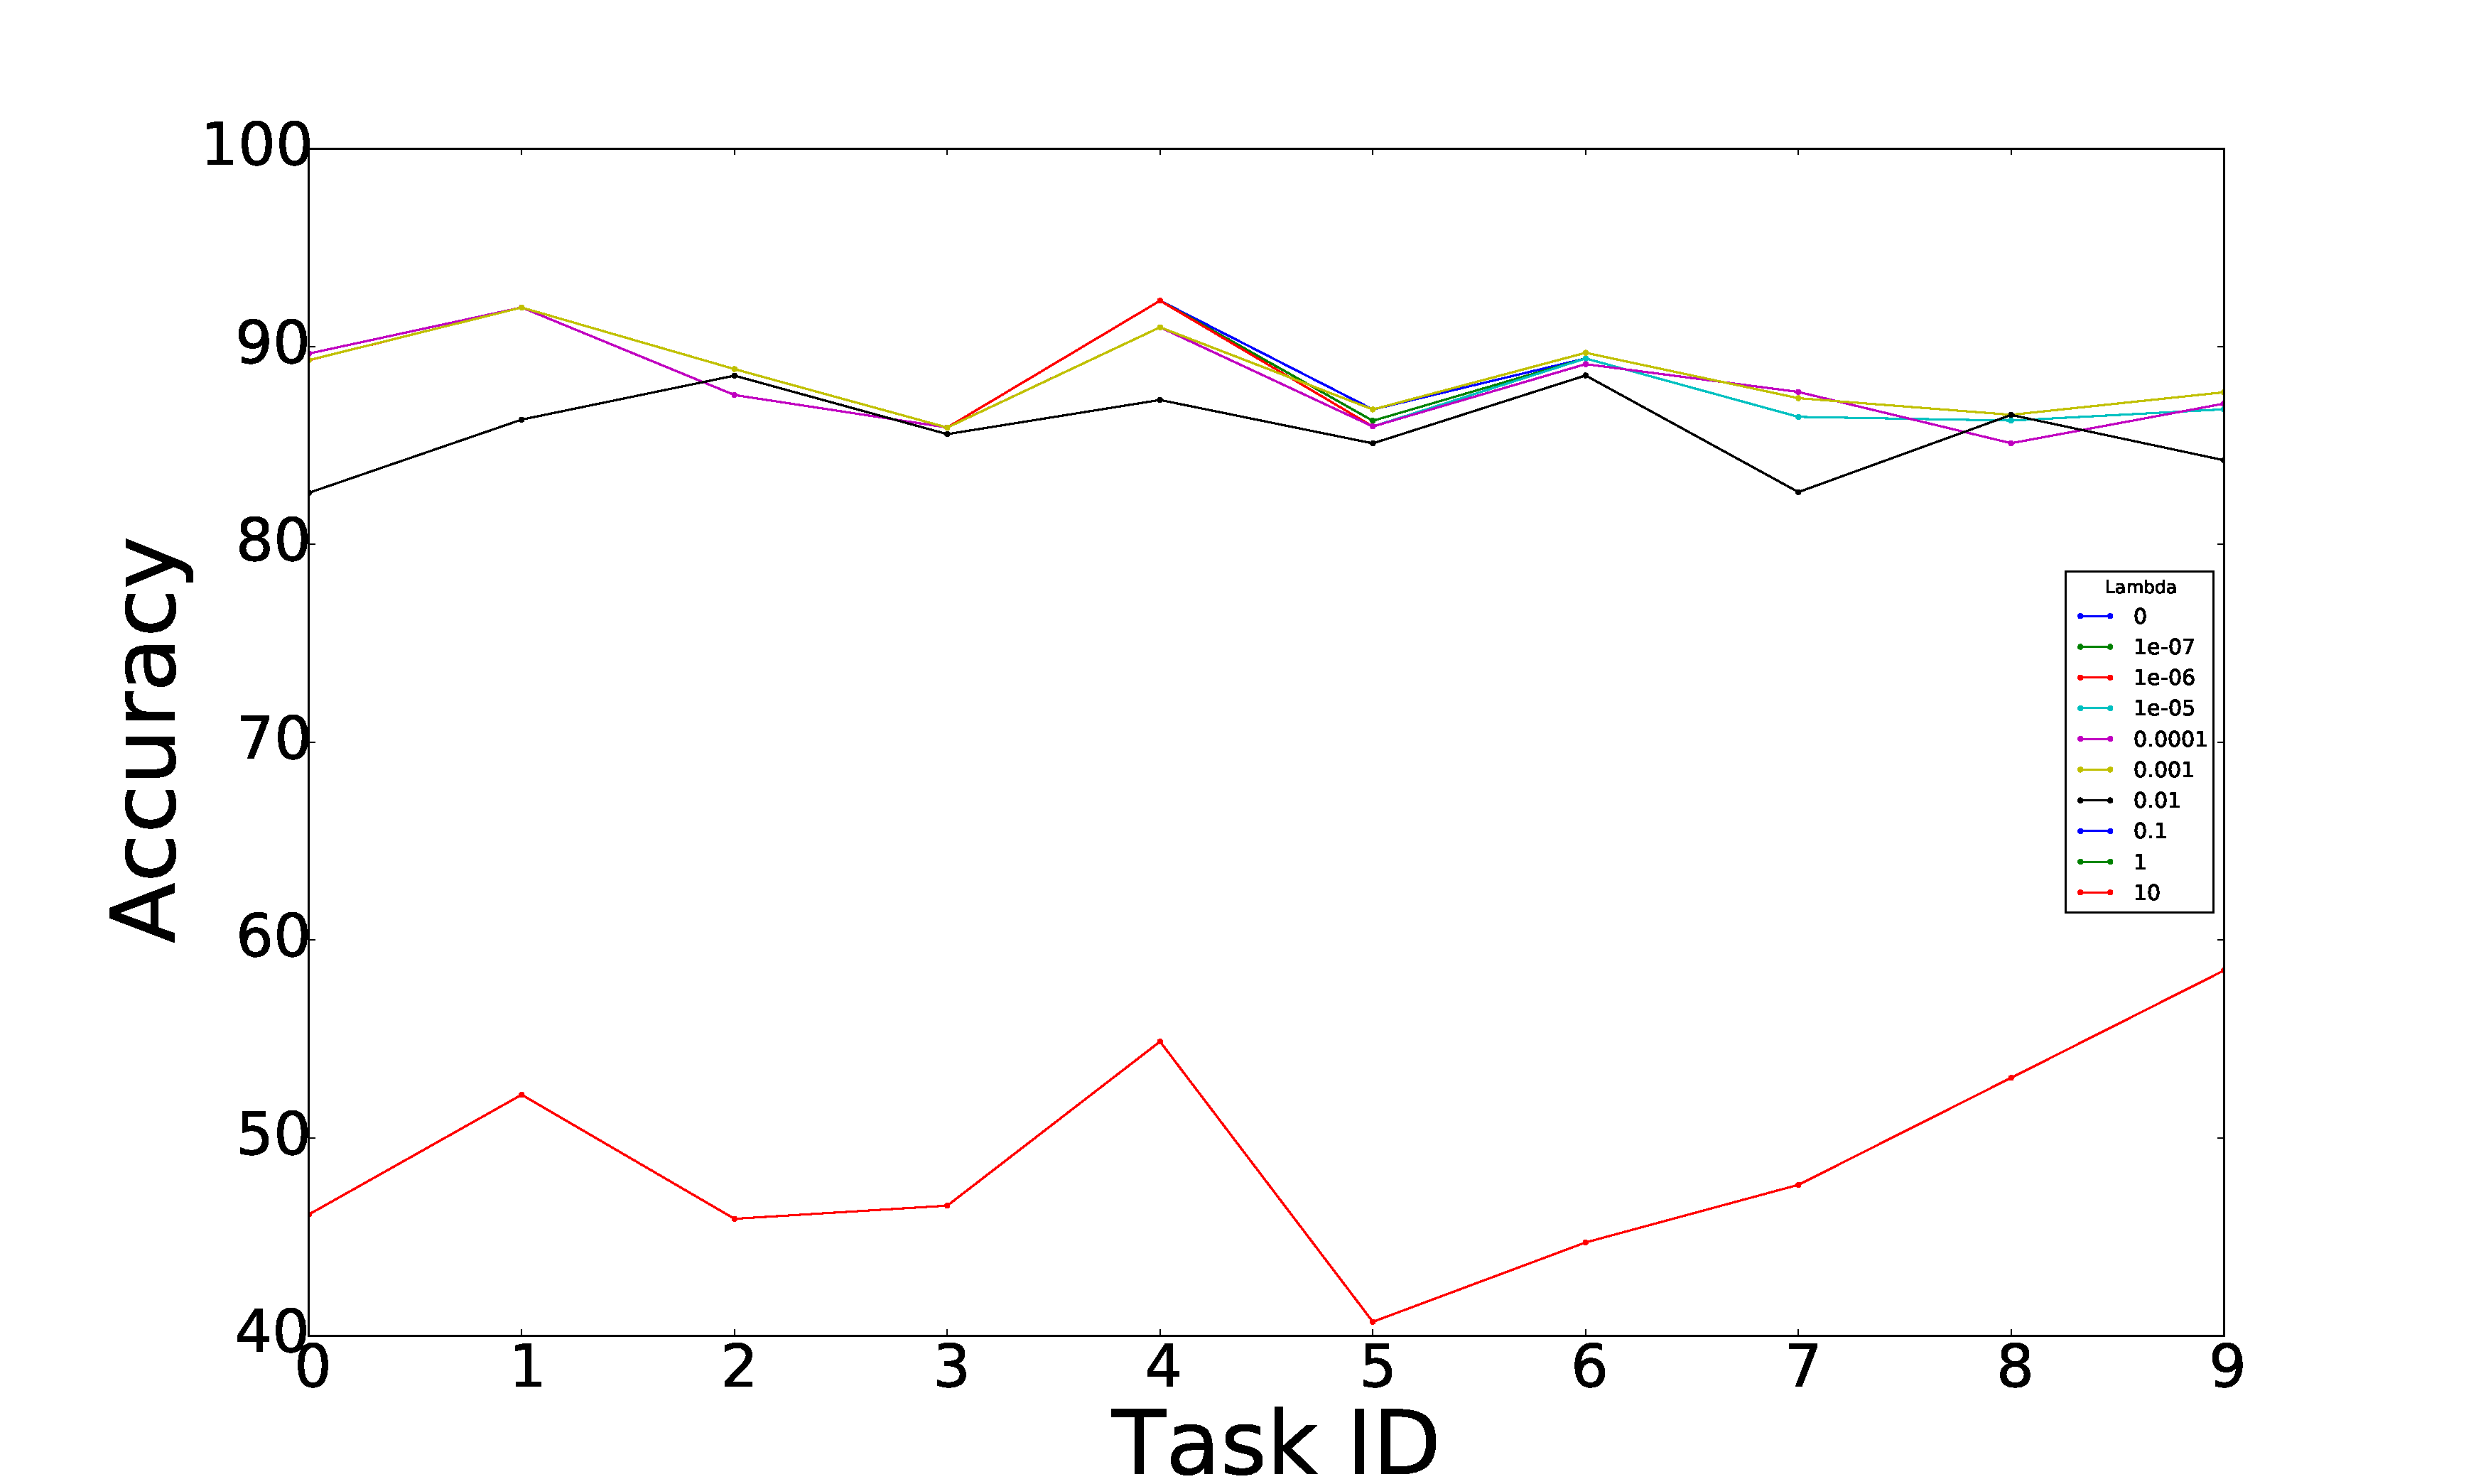
\includegraphics[width=\textwidth]{figures/accuracy_lambda}
        \caption{A gull}
    \end{subfigure}
    \begin{subfigure}[b]{0.45\textwidth}
        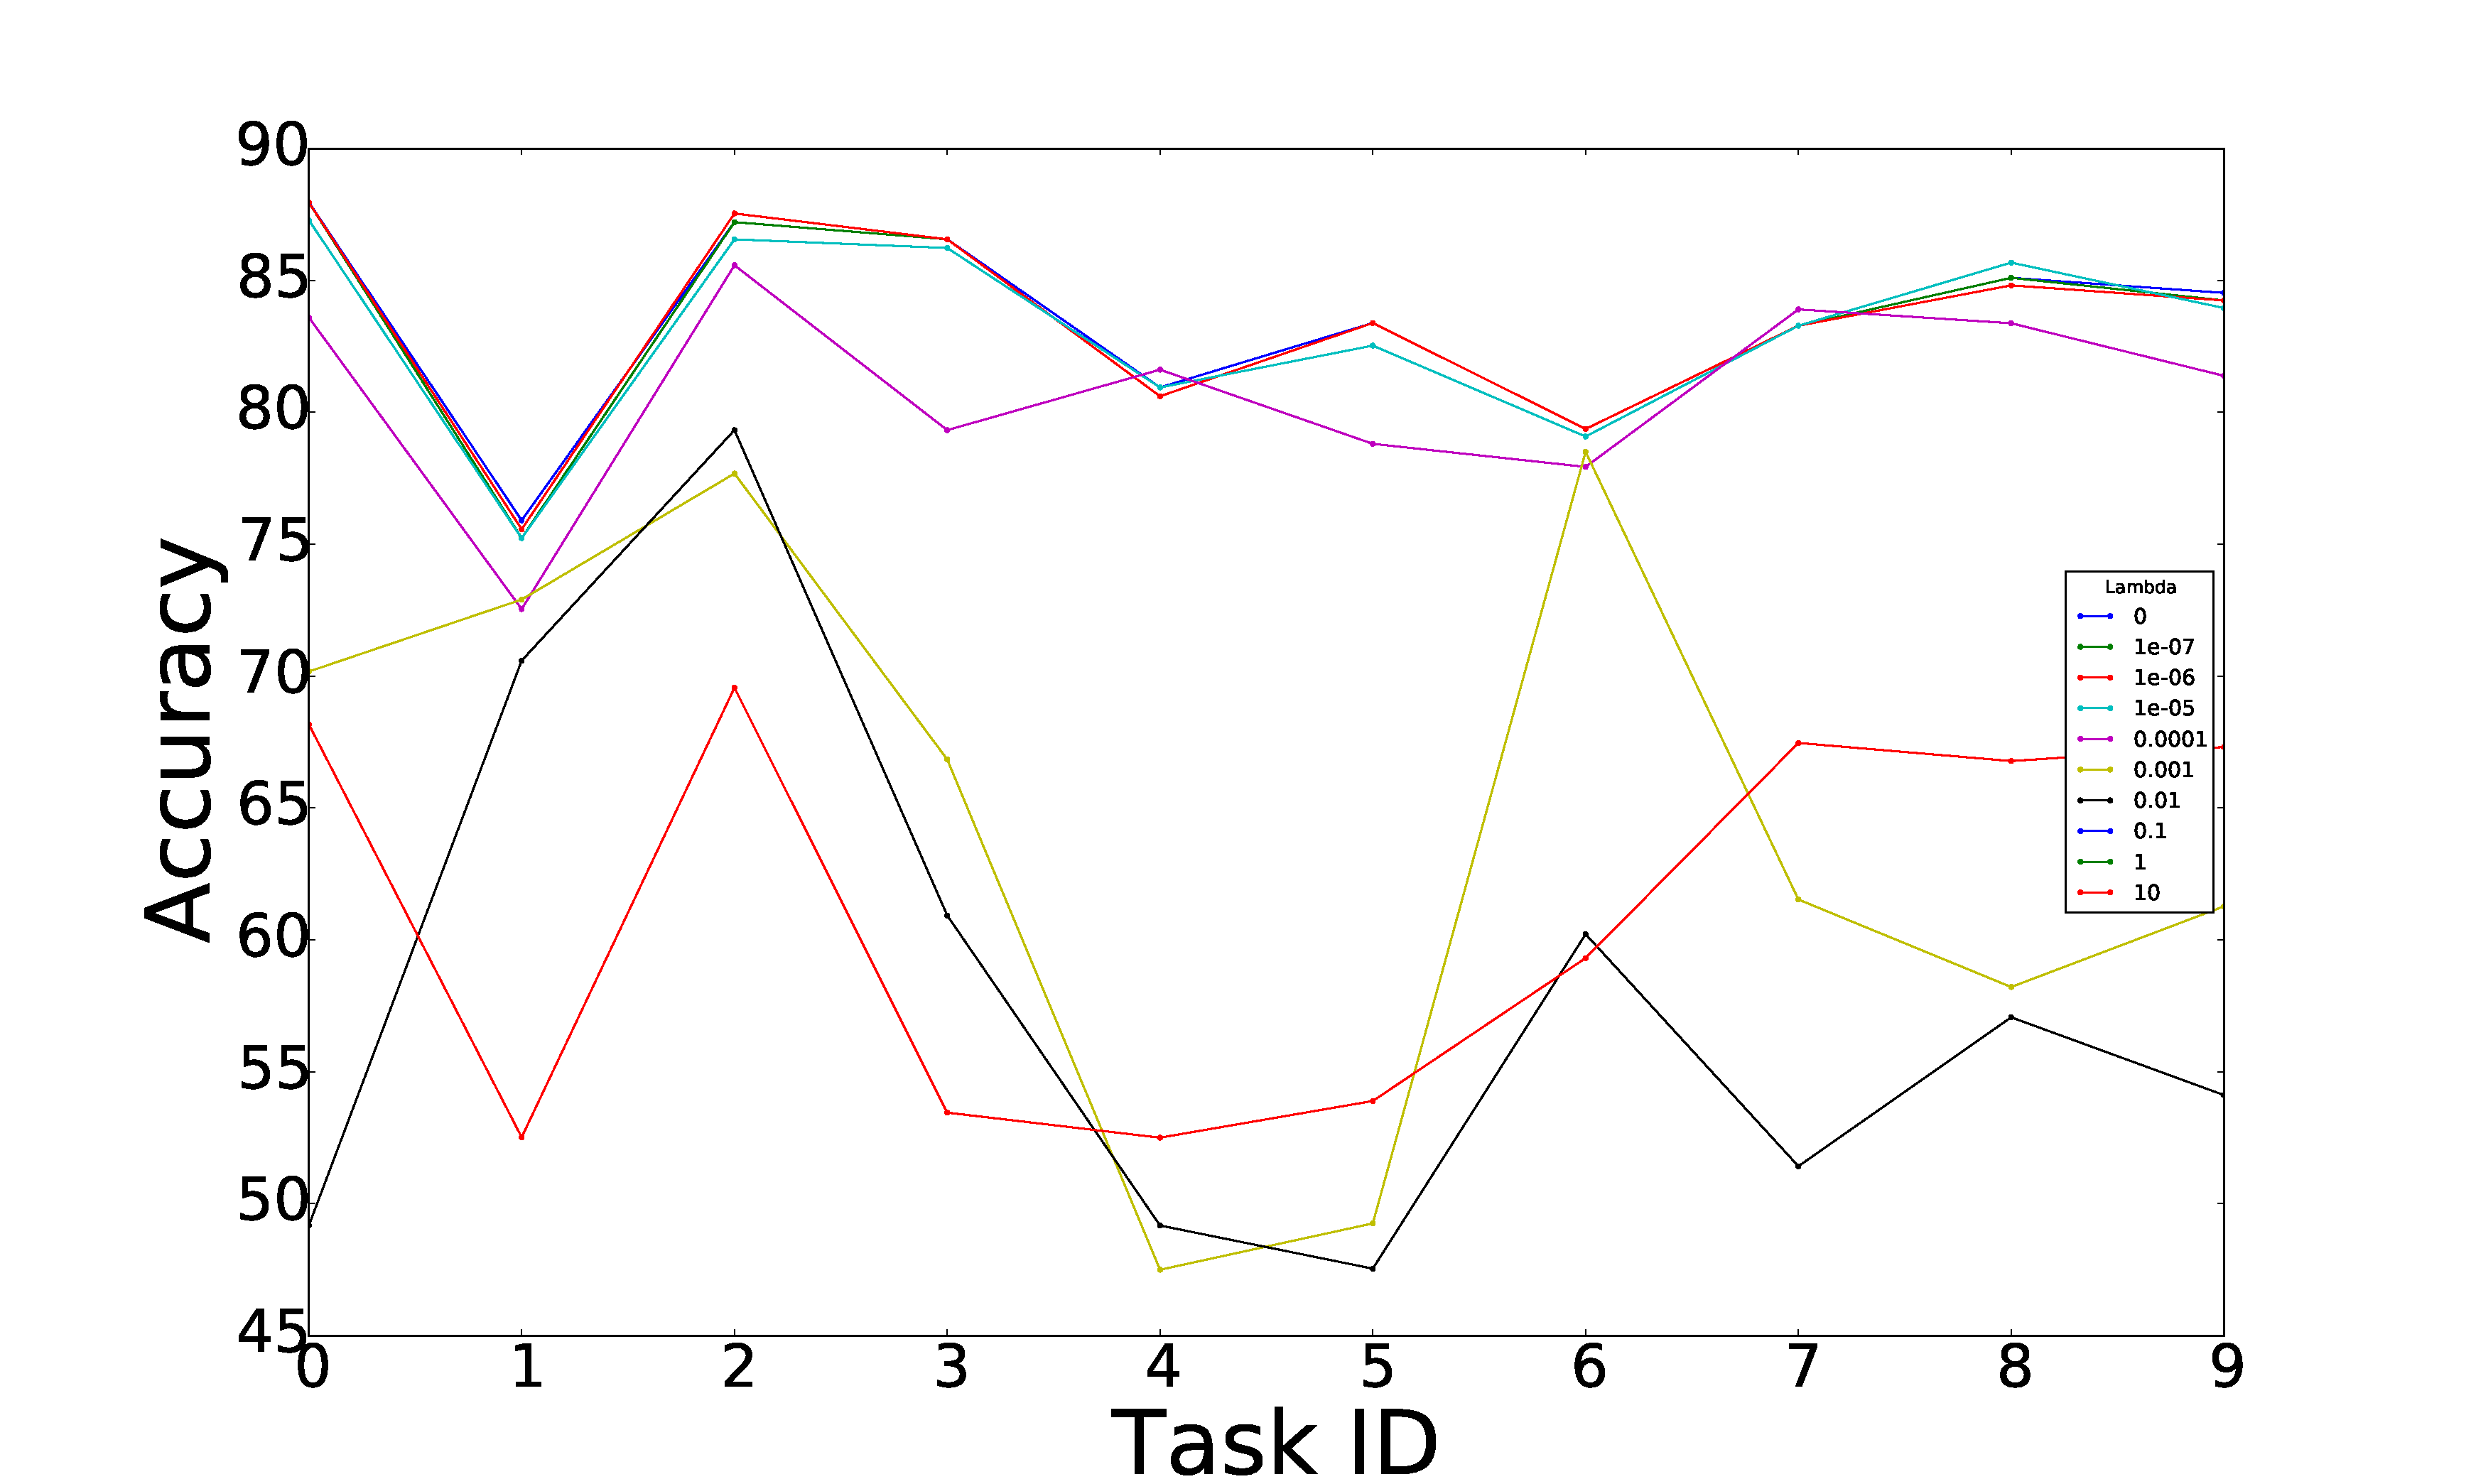
\includegraphics[width=\textwidth]{figures/accuracy_lambda_mlp}
        \caption{A gull}
    \end{subfigure} 
  \caption{Sensitivity to the hyperparameter}
  \label{fig:sensitivity}
\end{figure}




\subsection{Accuracy on synthetic data}

In this subsection we show the classification performance on our synthetically generated data. We show on \autoref{fig:synthetic}.that a small number of efficient labeling experts can give a much higher performance than individual labelers. 

\begin{figure}[!htb]
    \centering
    \begin{subfigure}[b]{0.45\textwidth}
        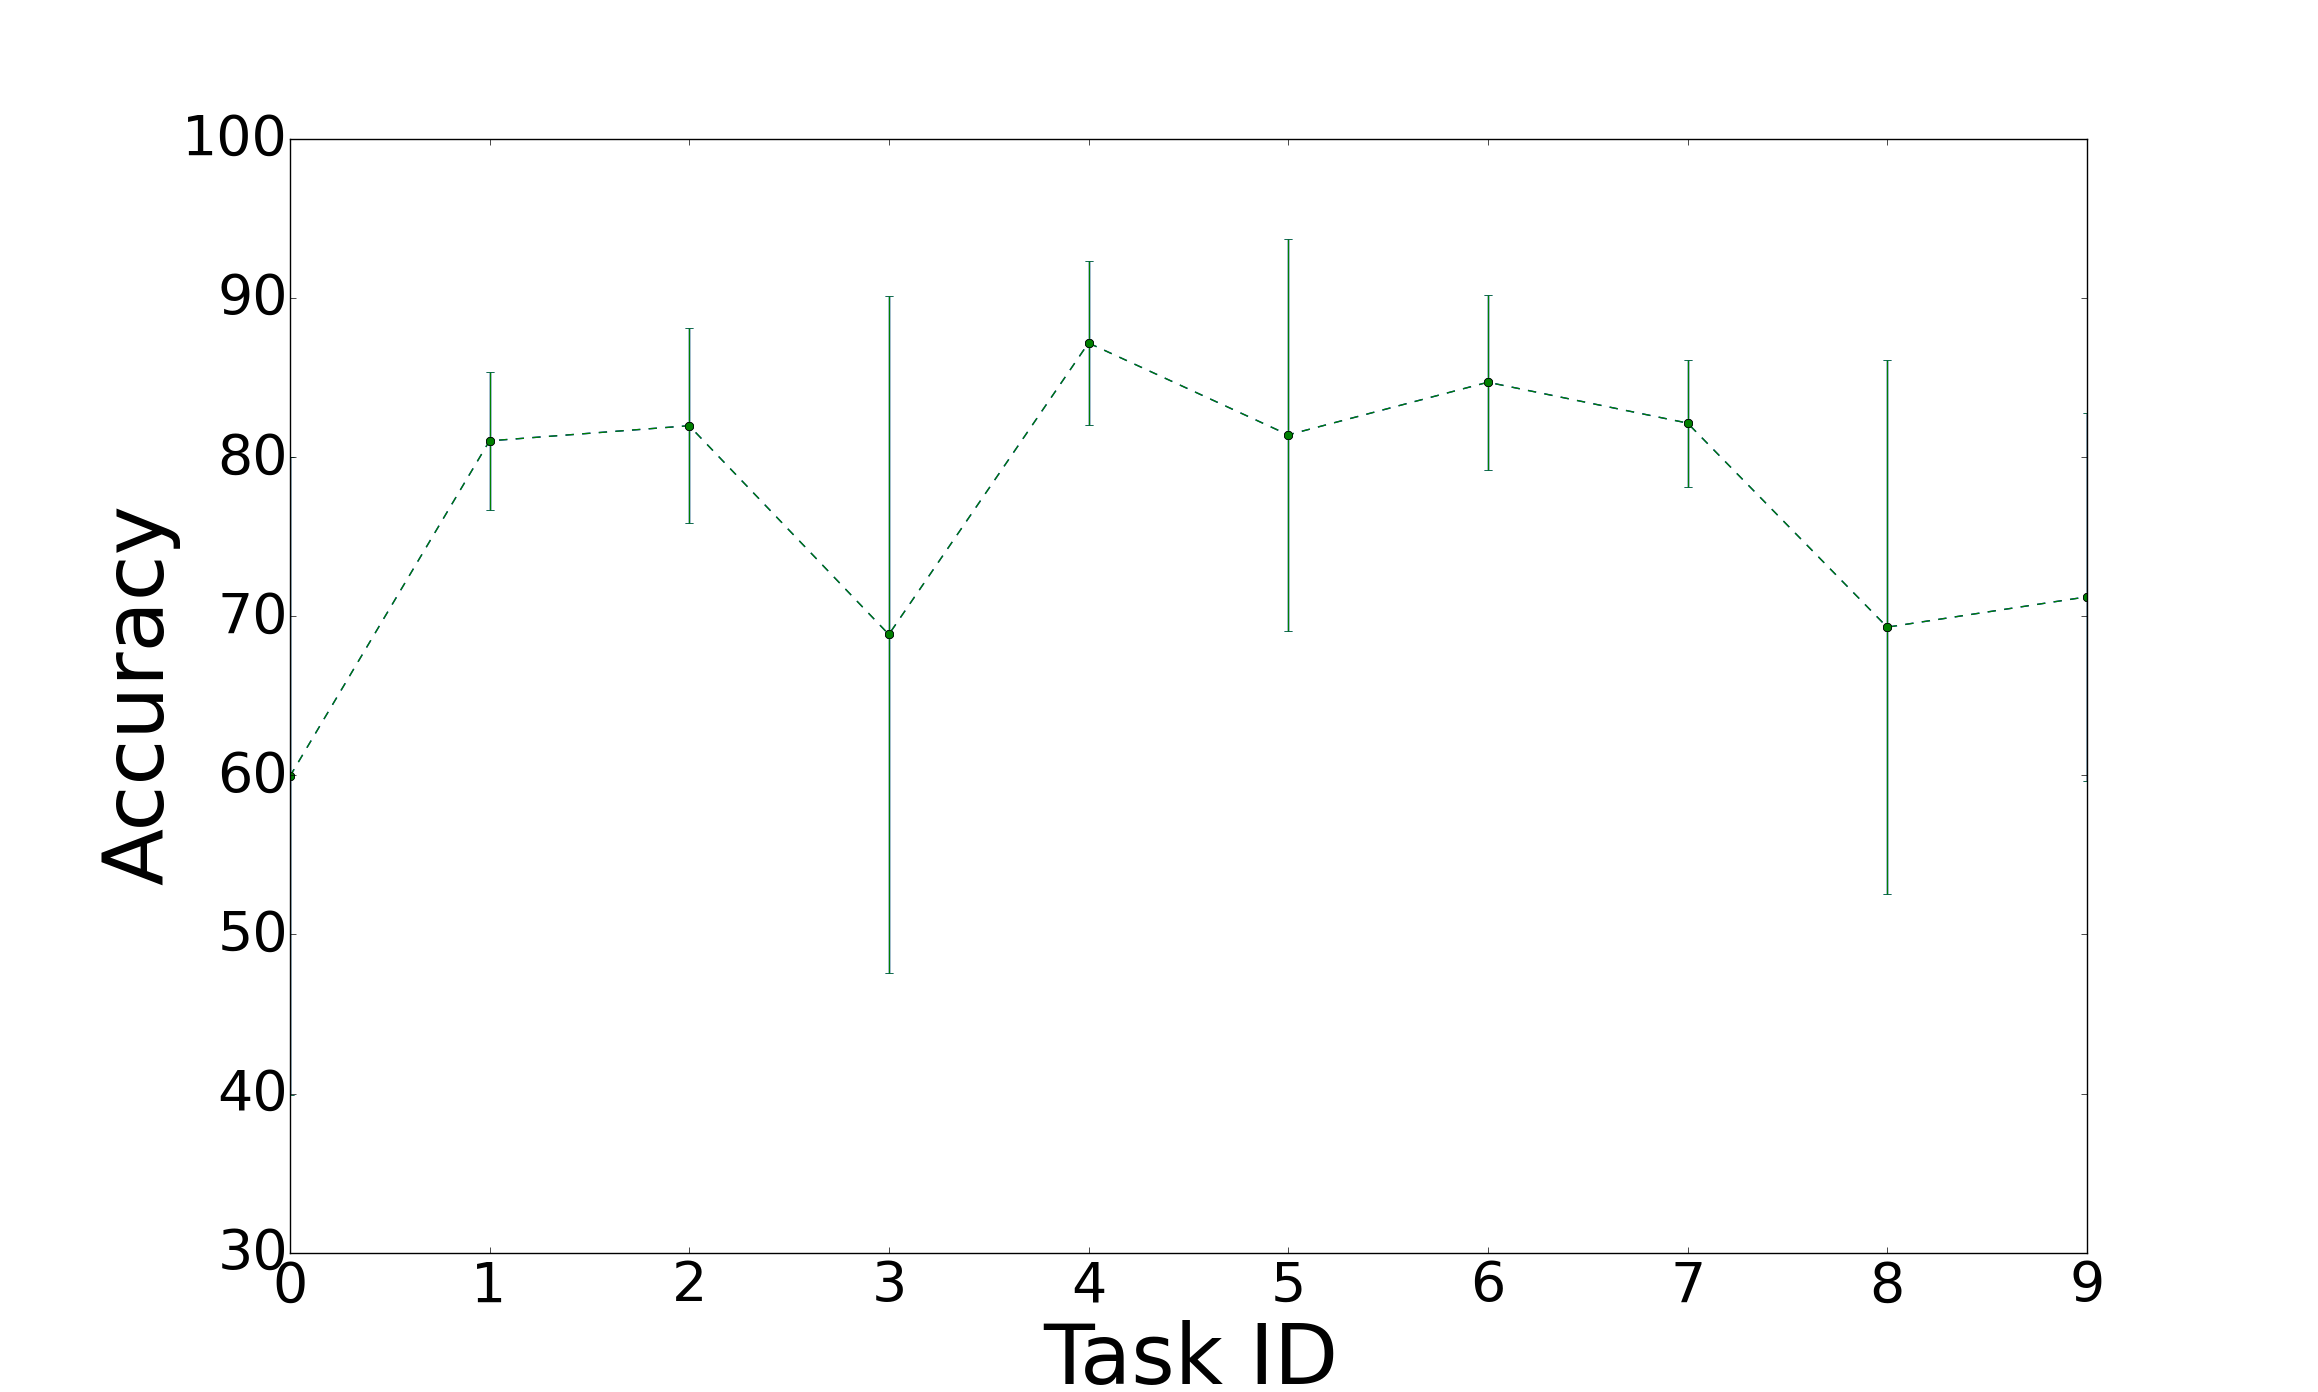
\includegraphics[width=\textwidth]{figures/plot_mlp}
        \caption{Logistic Regression}
    \end{subfigure}
    \begin{subfigure}[b]{0.45\textwidth}
        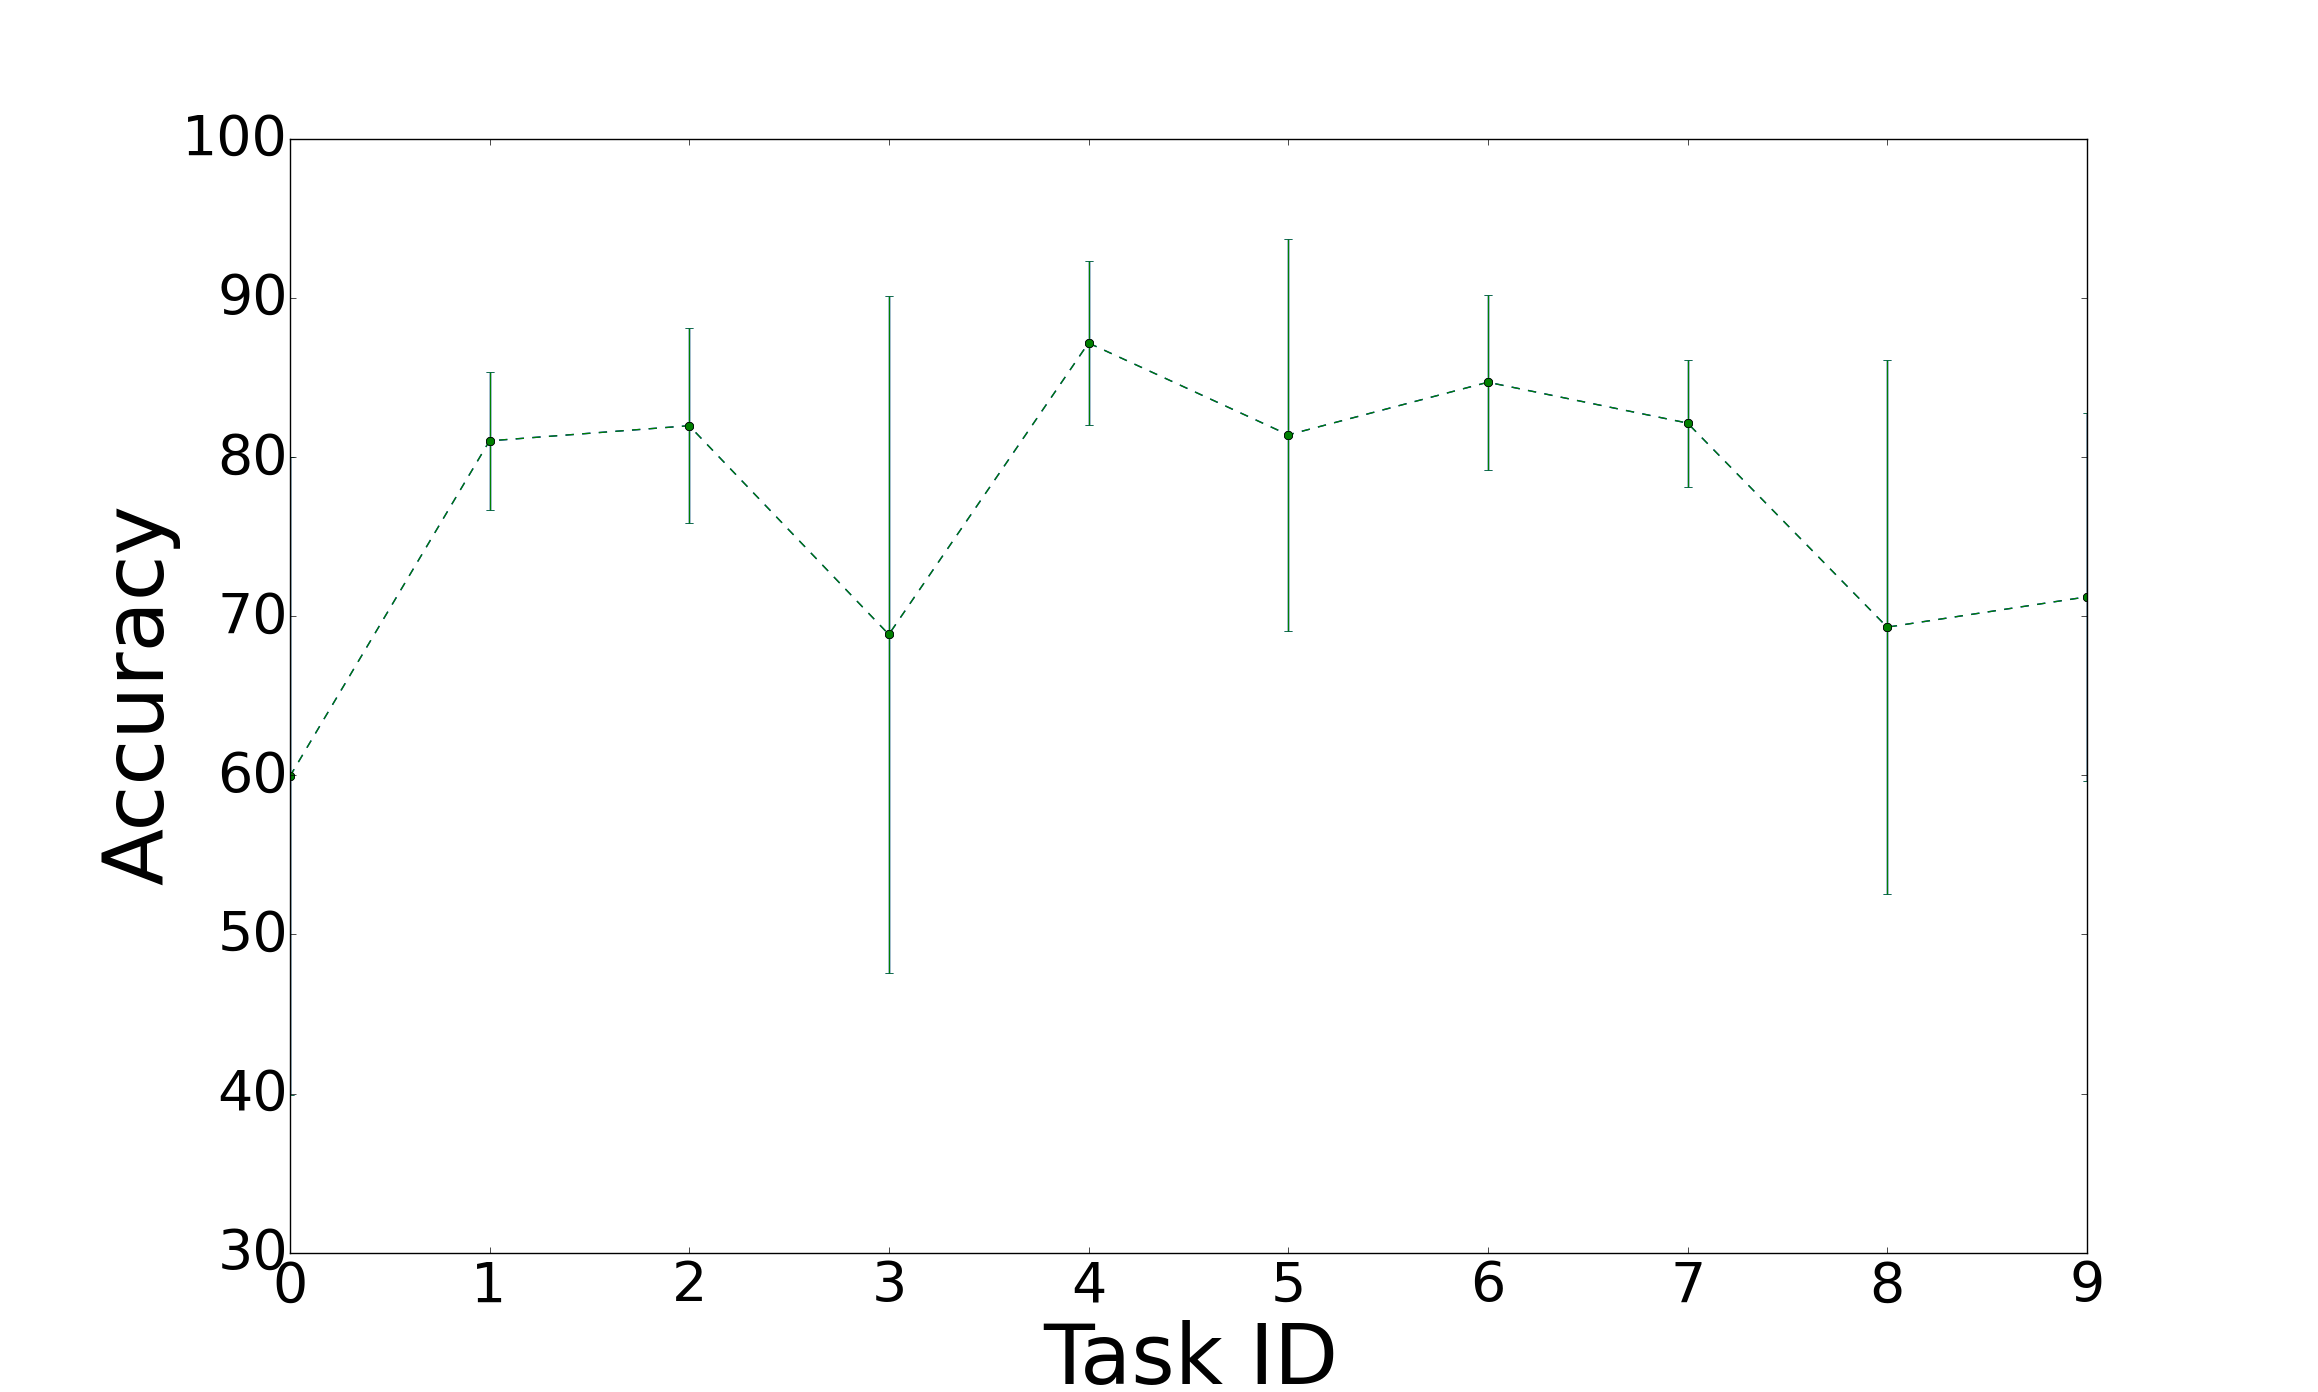
\includegraphics[width=\textwidth]{figures/plot_mlp}
        \caption{Neural Network}
    \end{subfigure}
  \caption{Accuracy for MNIST data}
  \label{fig:synthetic}
\end{figure}


\subsection{Comparison of sparse and dense vectors}

In the next figures we show the breakdown of performance for sparse selection w.r.t the selection with no sparsity enforcement. On \autoref{fig:sparsity_mnist} it is noticeable that the error rate is uniform.

\begin{figure}[!htb]
    \centering
    \begin{subfigure}[b]{0.45\textwidth}
        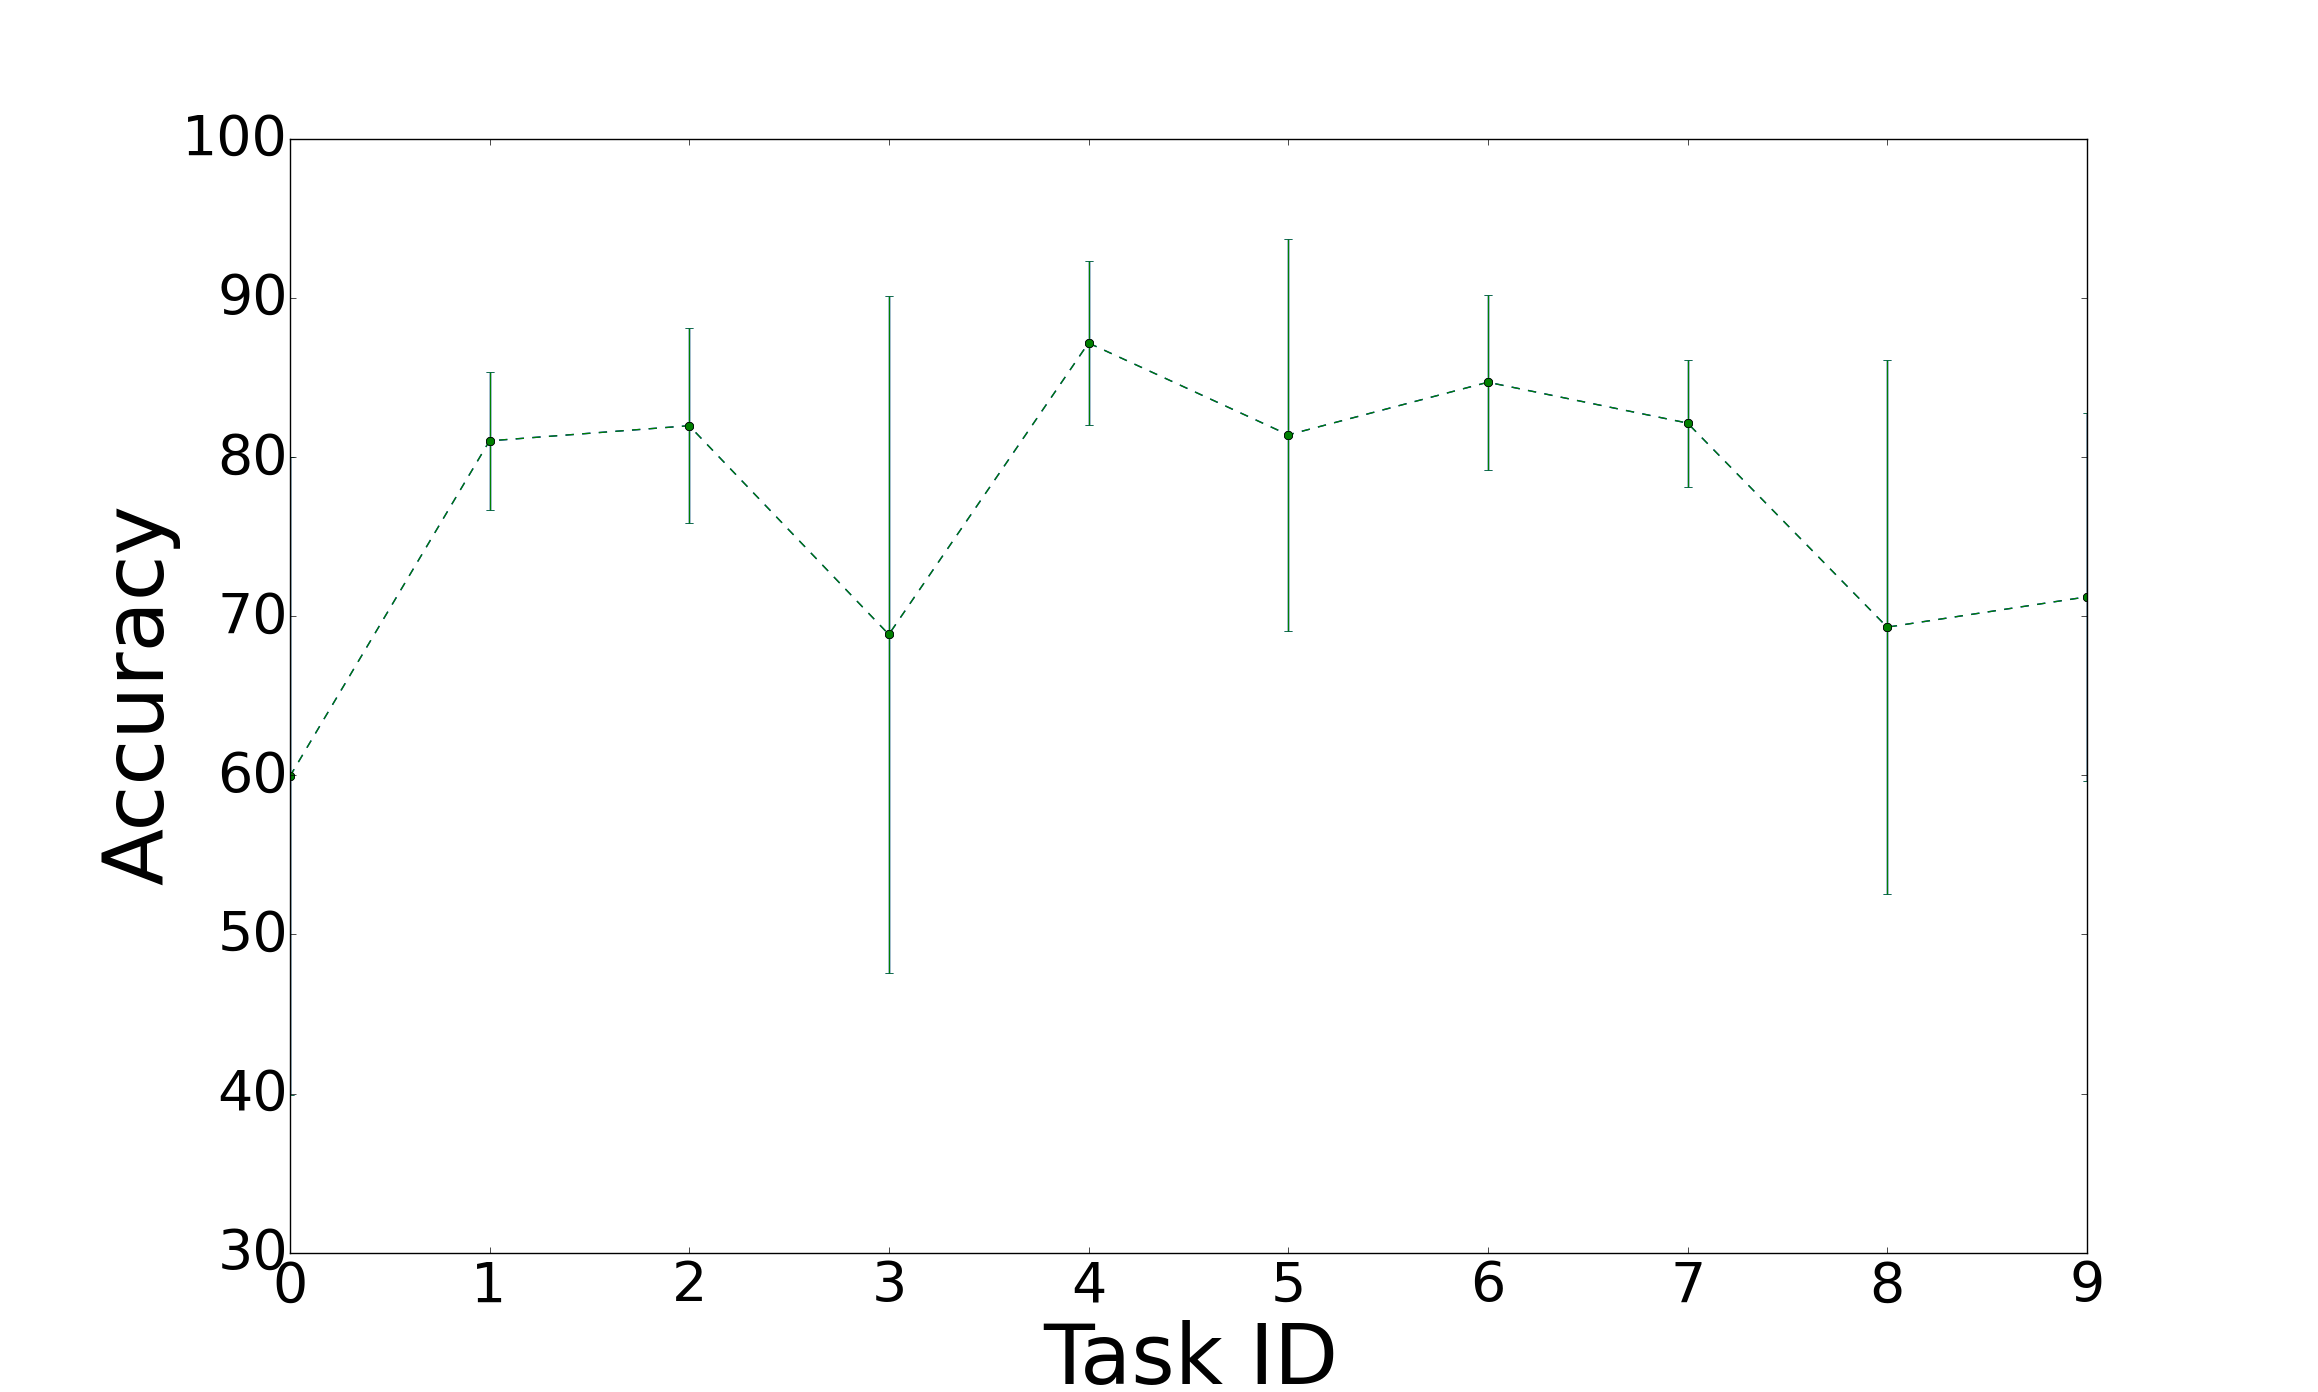
\includegraphics[width=\textwidth]{figures/plot_mlp}
        \caption{Logistic Regression}
    \end{subfigure}
    \begin{subfigure}[b]{0.45\textwidth}
        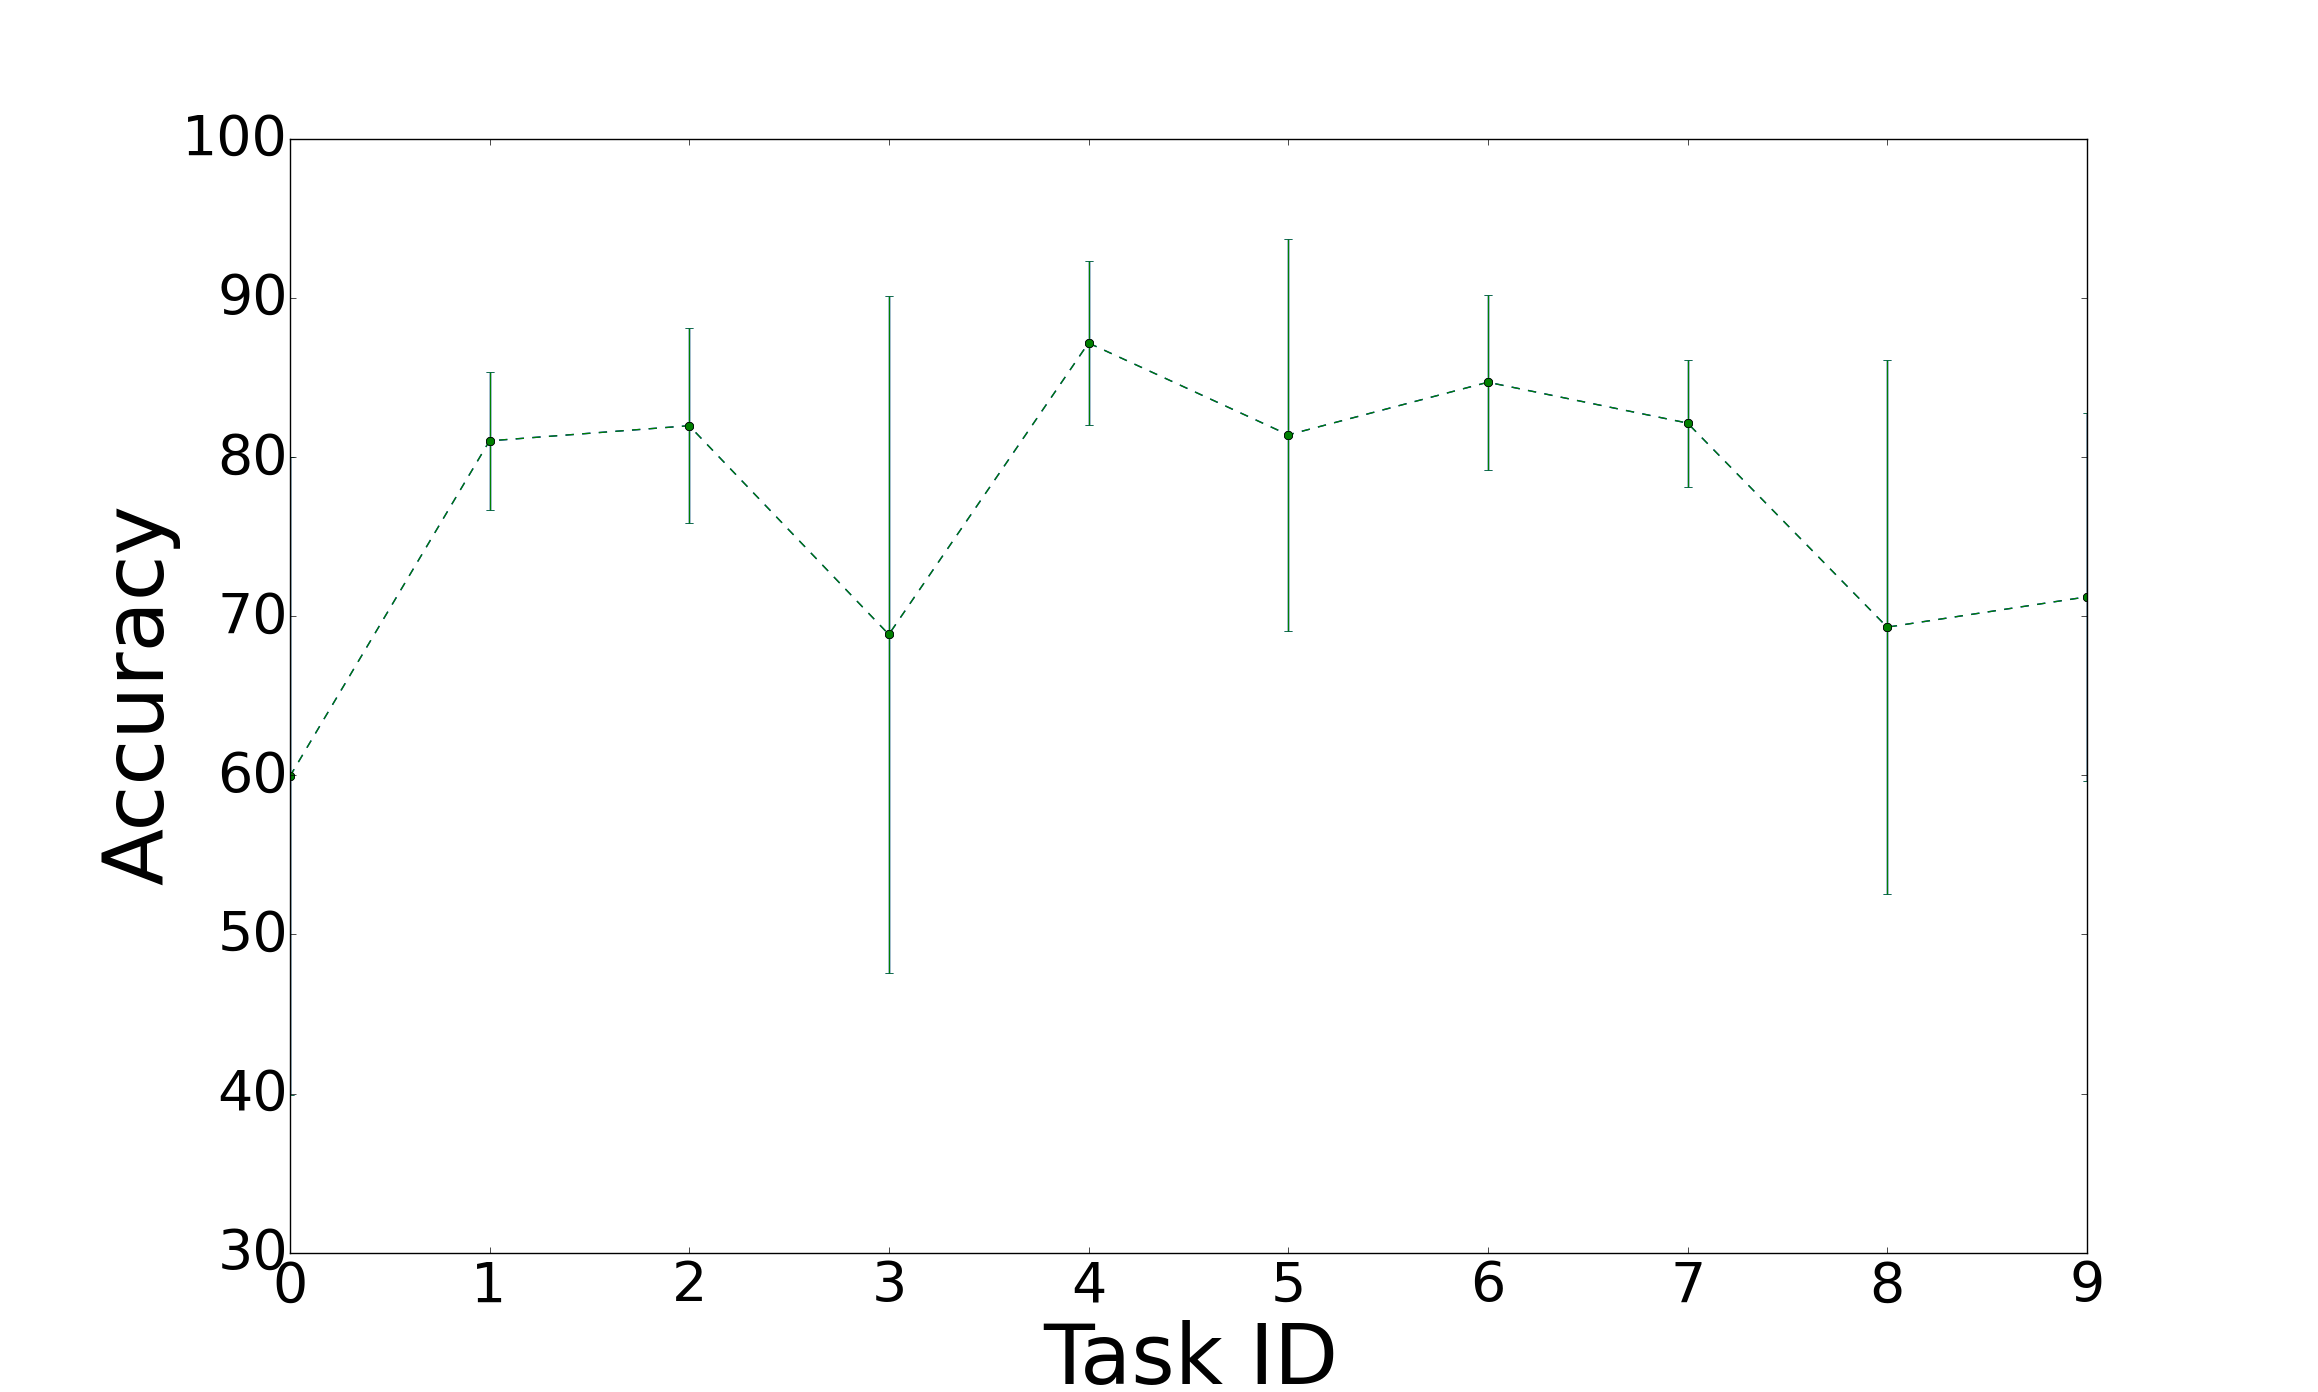
\includegraphics[width=\textwidth]{figures/plot_mlp}
        \caption{Neural Network}
    \end{subfigure}
  \caption{Performance per digit}
  \label{fig:sparsity_mnist}
\end{figure}



\subsection{Size of the annotator set}

In the next group of plots we show how the size of the annotator subset grows with the initial number of annotators. This is shown on  \autoref{fig:subset}

\begin{figure}[!htb]
    \centering
    \begin{subfigure}[b]{0.45\textwidth}
        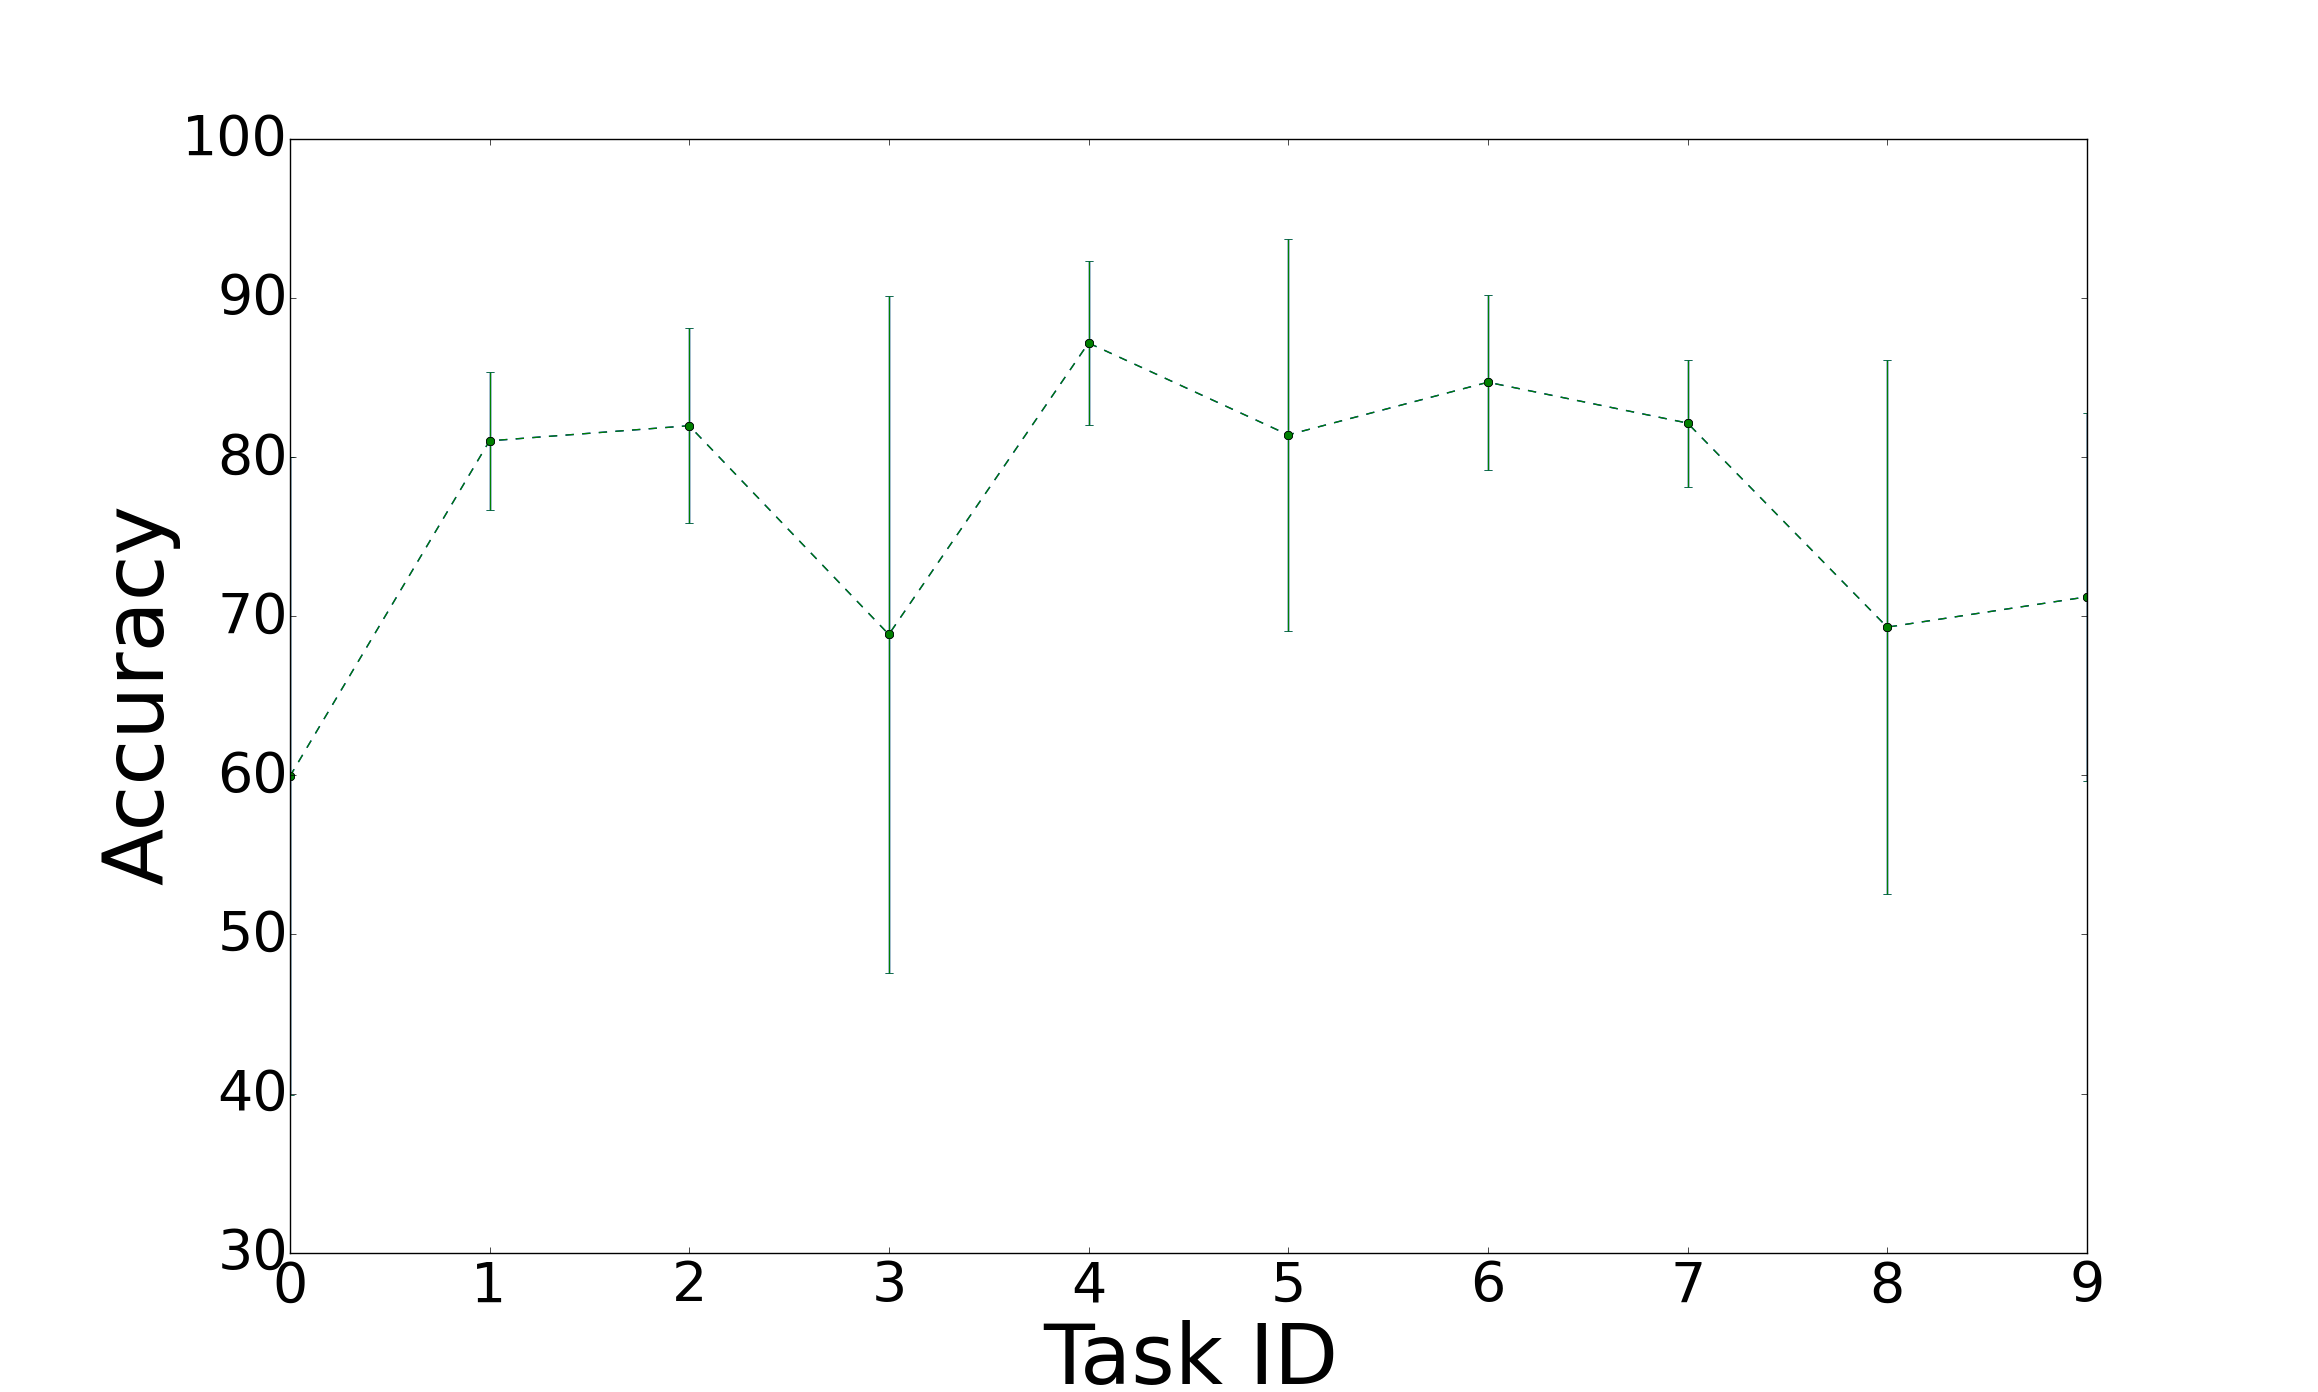
\includegraphics[width=\textwidth]{figures/plot_mlp}
        \caption{A gull}
    \end{subfigure}
    \begin{subfigure}[b]{0.45\textwidth}
        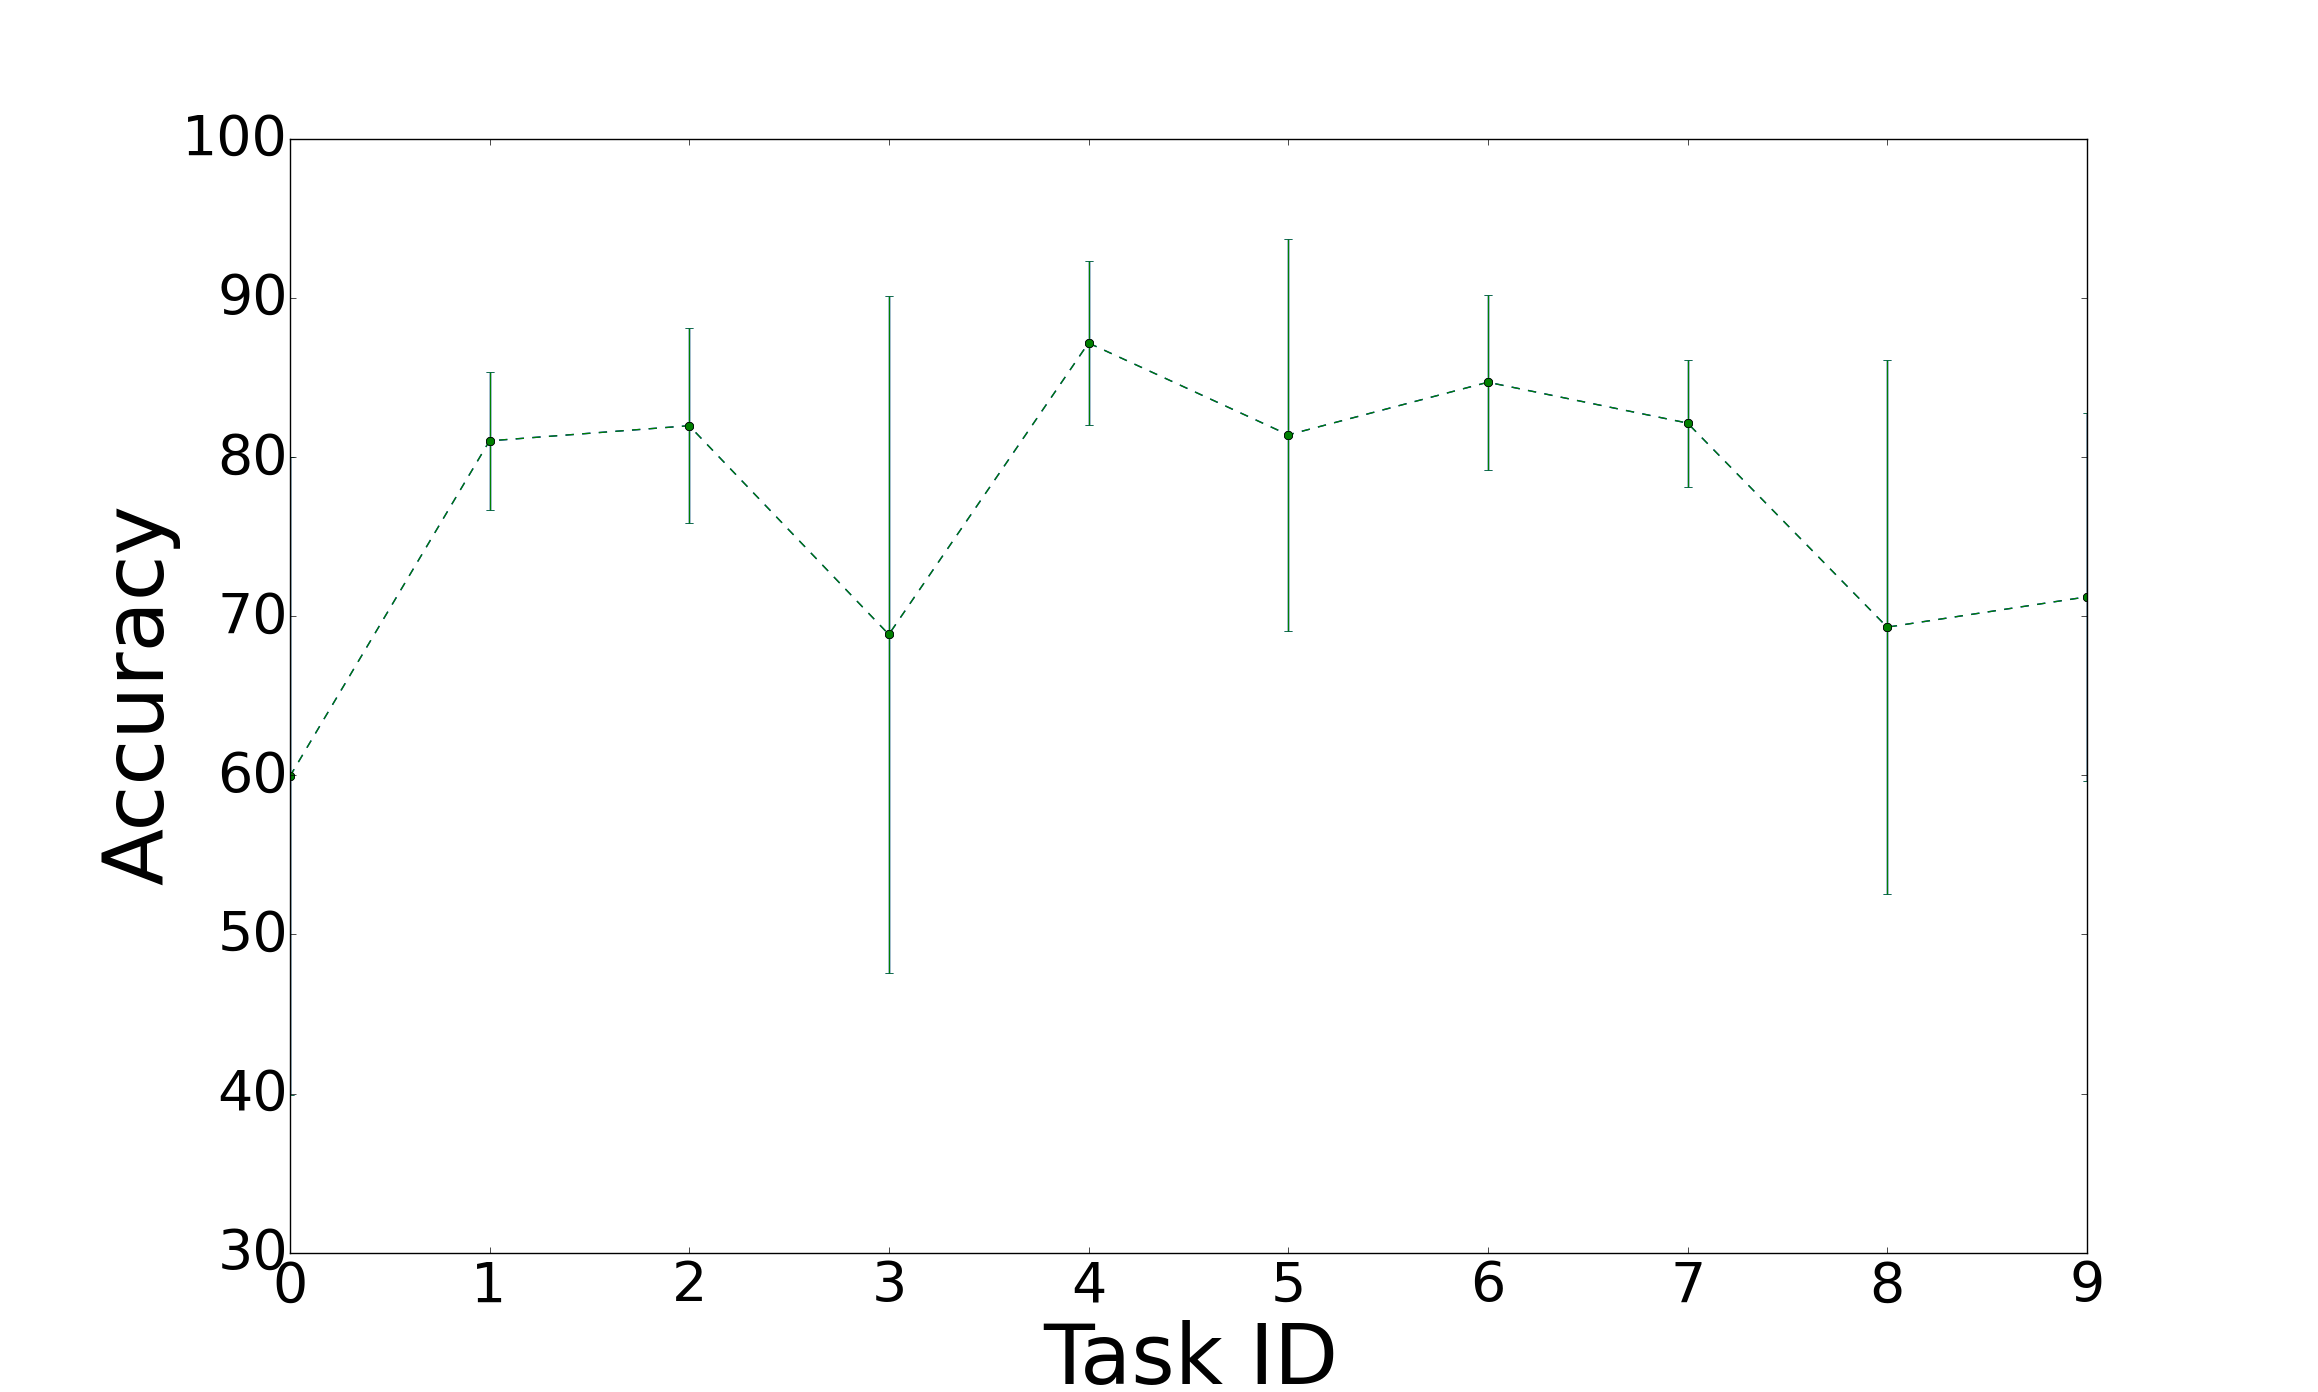
\includegraphics[width=\textwidth]{figures/plot_mlp}
        \caption{A gull}
    \end{subfigure}
  \caption{Change of size of the annotator groups}
  \label{fig:subset}
\end{figure}




\section{Discussion}


\section{Conclusion}


\section{Methodology}

In this section, we present the methodology we utilize for the continuous authentication. To achieve this we use four stages: $(i)$~experiment design, $(ii)$~data collection, $(iii)$~feature engineering and selection, and $(iv)$~online learning. In the following we present the threat model and each stage of building our authentication scheme.

\subsection{Threat Model}\label{ssec:threat}
In our methodology we consider the situation where we train our model incrementally using a valid user and then, in the test time, have both a valid user and an attacker trying to use the device. Both the attacker and the valid user leave a trace of their activity in the form of touchscreen interaction, accelerometer, and rotation sensor values. The goal of our system is to detect the attacker's behavior as a significant deviation from the model based on the valid user, while letting the valid user use the device without unnecessary interruption.  Therefore, we consider our problem as an example of unsupervised anomaly detection problems.

\subsection{Experiment Design}

To gather user-specific data, we design a two-part experiment focusing on different typical activities on the smartphone. For the first part, we focus on the simple activities consisting of a small set of touchscreen gestures. Therefore, we create a mobile app for Android 5.0, specifically designed and implemented for this purpose. We instruct users to execute actions on a smartphone based on the following gestures: swipe, keystroke, double tap, and pinch. For the second part, we leverage mobile apps that are typically used by smartphone users. We instruct users to perform some actions on popular smartphone apps in order to collect their sensor value patterns when using these applications.

\medskip \noindent \textbf{\emph{Requested Tasks in our Mobile App.}}
We request users to perform a series of tasks so we can train our model. A potential future app, delivered directly from the smartphone vendor, could offer the option for users to train their smartphones with their behavior, if they wish to enable the continuous authentication feature. Another possibility is for the user to perform the tasks presented in our app under the hood. This means that the phone does not need to execute an application, where it requests input from the user, but it can stealthily collect data and train the models. The tasks that we use for collecting continuous authentication data in our app are the following:

\begin{enumerate}
%
\item \emph{Image Finding.} We show the users 20 pictures in a row. By using horizontal and vertical scrolling they should find one particular image given in the instructions. The correct picture is then selected by a double tap.
%
\item \emph{Text Reading}. The user is asked to first read a text. To read the whole text they have to scroll down (or perhaps scroll up in case they miss some information). After reading the text, they have to answer five questions, which are displayed below the text.
%
\item \emph{Zooming.} We display a picture together with a corresponding question about a specific detail. The picture is either zoomed in or zoomed out so that the users could not find the detail without zooming the picture to the appropriate screen size. %We repeat this task ten times with different pictures and details.
%
\item \emph{Message Composition.} In this task, we ask users to enter a message and a recipient. %The data is given on the task description handed out to participants.
This way, we emulate users' behavior when composing an email or a SMS message.
%
\item \emph{PIN.} We ask users to enter a four-digit PIN five times in a row. The repetition makes the user adding the PIN more natural, similr to what happens in real-life.
%
\item \emph{Phone Call.} After having entered a given phone number correctly, users have to press the call button. In total three phone numbers are given, making the users repeat the task for each number.
%
\end{enumerate}

We design these tasks taking into account the most often performed activities on a smartphone. Each task is repeated at least ten times per participant which lowers the risk of sudden change of behavior because of external conditions (e.g. stress).

\medskip \noindent \textbf{\emph{Tasks with Built-in Apps.}}
We execute the next series of tasks using the apps provided by the mobile devices themselves. This makes the behavioral traces of users more natural, as they regularly use this kind of apps and can perform the tasks more smoothly.

\begin{enumerate}
%
\item \emph{Browsing.} We ask users to search on Google and read three specific Wikipedia articles. To verify that users read the correct articles, they had to type a correct answer to three questions about the corresponding paragraphs.
%
\item \emph{Taking a Selfie.} Users are asked to take a selfie with the smartphone camera.
%
\end{enumerate}

\subsection{Data Collection}

We used the \textit{Samsung Galaxy S4} smartphones with Android 5.0 to execute the above described experiments with 28 participants in order to capture the discriminative features in user activity.

\medskip \noindent \textbf{\emph{Motion Events.}}
The Android API delivers a sequence of motion events to the currently active application each time a user touches the screen. The touch sequence is started by a down event followed by a variable number of move events and an up event closing the sequence. Each motion event can be identified by its timestamp and its $x$ and $y$ coordinate. Timestamps are reported in \textit{ms} since the last reboot of the device. Besides, major and minor axis of the ellipse making up the touch contact are reported as well as the approximate size of the contact area. The size is calculated as mean of major and minor of the ellipse axes. To distinguish different types of events, we label them with an event ID. To support multitouch, each event is additionally labeled with a pointer ID to distinguish events caused by different fingers on the screen.

\medskip \noindent \textbf{\emph{Custom Keyboard.}}
For security reasons our version of Android does not allow to capture keyboard input of the standard keyboard. Therefore a custom keyboard is developed that resembled the Samsung keyboard, which was running as an Android service. Users are instructed to choose the custom keyboard when opening the app such that no other keyboard could accidentally be used. Apart from the motion events described in the previous subsection, the keycode of each key hit is captured.

\medskip \noindent \textbf{\emph{Sensor Service.}}
In addition to touch data, sensor data from built-in accelerometer and gyroscope (rotation sensor) is harvested. Data is polled at a rate of five times a second. The accelerometer measures acceleration in \textit{m/s2}, while the gyroscope measures rate of rotation in \textit{rad/s} along $x$, $y$ and $z$ axis of the phone. Gathering sensor data is done by running an Android service, same as in case of the custom keyboard.

\medskip \noindent \textbf{\emph{Input Device Driver.}}
Android only allows capturing touch events from within a custom application. Therefore, it is not possible to gather motion events from the Android API while using standard applications for the second part of the experiment. Nevertheless, it is possible to directly read from the input device driver under /dev/input/eventX, where X is a number identifying the input device. Whenever the user leaves the app, touch events are automatically read from the input driver: it reports a stream of single values not processed to higher level motion events as in case of the Android API. Each value is reported with its timestamp, a label identifying the type of input, and its actual hexadecimal value. The types of inputs are: $(i)$~$x$ and $y$ coordinates, $(ii)$~major and minor ellipse axis, and $(iii)$~a pointer counter that is increased each time a finger hits the screen. Since the devices used in this study are not capable of directly recording the user's pressure when touching the screen, we could not evaluate this feature. Although we could not measure this pressure directly, acceleration in $z$-direction together with touch area size gives information about the device's response to the force applied to the screen.

\subsection{Feature Engineering and Selection}

Using ideas from related work, we capture a large range of spatio-temporal features to determine which subset is the most useful. There are 59 features from swipe gestures and 51 features from keystrokes. The swipe feature set contains data that characterizes the trajectory of the swipe motion, the velocity of movement, and size of the trace. On the other hand, the keystroke features contain the similar velocity and stroke size patterns as well as keycode and offsets to the key center. Our feature set is based on the works of Velten et al~\cite{velten2015user}, Frank et al.~\cite{Frank13}, and Buschek et al.~\cite{buschek2015}.

Before training the model we execute a simple feature selection process. Our feature selection is based on the sequential feature selection procedure. According to the sequental feature selection algorithm~\cite{ruckstiess2011sequential}, in each round $k$ the feature is added to the feature subset $Y_k$ that yields highest classification accuracy $J( Y_k )$. Starting with the empty set, we compare classification accuracy for each feature that has not already been added to our feature subset in previous rounds. This has been done for 30 differently sampled user combinations. The feature that is chosen by most of the validation tests is added. If features yield same results one is randomly selected. We execute this procedure for the keyboard and swipes data separately.


\subsection{Online Learning}

This section introduces the notation used throughout the paper. A summary of notation can be found in Table~\ref{tbl:notation}.

\begin{table}
\centering
\begin{tabular}{lll}
	\toprule
	\textbf{Notation}       &   & \textbf{Explanation}                               \\ \midrule
	$x^{t}$                 & : & Incoming sample at time t                          \\
	$x_{i}$                 & : & $i$-th support vector                               \\
	$K(\cdot,\cdot)$        & : & RBF-kernel                                         \\
	$\gamma$                & : & Kernel parameter                                   \\
	$f_{t}$                 & : & Model at time $t$                                  \\
	$\alpha_{i}$            & : & Weight for $i$th support vector                    \\
	$y^{t}$                 & : & Correct class label at time $t$                    \\
	$\hat{{y}}^{t}$         & : & Predicted class label at time $t$                  \\
	$\ell(f;(x^{t},y^{t}))$ & : & Loss function                                      \\
	$B$                     & : & Budget size limiting the number of support vectors \\
	$X$                     & : & Set of support vectors                             \\
	$margin$                & : & Distance from decision boundary                    \\ \bottomrule \\
\end{tabular}
\caption{Summary of notation.}
\label{tbl:notation}
\end{table}

\begin{comment}
%
\begin{minipage}{0.3\textwidth}
	\vspace{\baselineskip}
	$x^{t}$\\
	$x_{i}$\\
			$K(\cdot,\cdot)$\\
			$\gamma$\\
			$f_{t}$\\
			$\alpha_{i}$\\
			$y^{t}$\\
			$\hat{{y}}^{t}$\\
			$\ell(f;(x^{t},y^{t}))$\\
			$B$\\
			$X$\\
			$margin$\\


\end{minipage}
\begin{minipage}{0.7\textwidth}
	\vspace{\baselineskip}
	Incoming sample at time t\\
	$i$th support vector \\
	RBF-kernel \\
	Kernel parameter\\
	Model at time $t$\\
	Weight for $i$th support vector\\
	Correct class label at time $t$\\
	Predicted class label at time $t$\\
	Loss function\\
	Budget size limiting the number of support vectors\\
	Set of support vectors\\
	Distance from decision boundary\\

\end{minipage}
\end{comment}

Xu et al.~\cite{xu2014towards} have shown that user behavior is not stable over time. To be able to continuously authenticate a user, we need our model to adapt to the current behavior. For this reason batch learning techniques are inappropriate in this setup, as they rely on training data being available in advance. They are not able to adapt to changes occurring after the initial training phase. Instead, the model should change whenever needed as well as be constantly evaluated in characterizing current user behavior. Online machine learning therefore constitutes a logical solution.

Algorithm~\ref{alg:online} introduces the basic online learning principle. Instead of training only once on a larger data set, online learners learn incrementally whenever new data is available. As they are only presented one sample at a time, online learners need to efficiently deal with limited information: they continuously adapt their learned decision boundary to the incoming stream of data. On receiving a new sample $x_{t}$ at time t, they predict its class label based on the current model $f_{t}$. Afterwards, they compare the retrieved label to the true class label given after the prediction and update the model. Many of the models are built in a nonparametric way to become more flexible.

 \begin{algorithm}[H]
 	\caption{Online Learning}
 	\label{alg:online}
 	\begin{algorithmic}[1]
 		\For{t = 1,2, ... }
 		\State receive instance $x^{t}$
 		\State predict label: $\hat{{y}}^{t} = sign(f_{t}(x^{t}))$
 		\State receive correct label $y_{t}$;
 		\State update model;
 		\EndFor
 	\end{algorithmic}
 \end{algorithm}

However, nonparametric online methods suffer from unlimited growth of the model over time. As we concentrate on bounding memory requirements in this study due to the resource-constrained environment on the device, we aim to to limit the model size. The next section introduces an online algorithm on a budget that is able to limit the number of support vectors and meet this requirement. For comparison, online learning algorithms with unlimited budget will also be tested 
in Section~\ref{sec:evaluation}.



\subsection{Budgeted Online Learning -- Classification decision}
Classifiers separate classes based on a learned decision boundary. The decision boundary is represented by a hyperplane that is defined by a set of weighted support vectors. Since data need not be linearly separable into classes by means of a linear model, we can make use of the kernel trick and make our model nonparametric. This allows us to transform the model into a different feature space where data may be separable. In this study we use the well-known RBF-kernel (Radial Basis Function), defined as:
\begin{equation}\label{eq:kernel}
K(x^{t},x_{i})=exp(-\gamma||x^{t}-x_{i}||^{2}), \: K(x^{t},x_{i})\: \in [0,1],
\end{equation}
with $\gamma$ set to 0.5. The RBF-kernel measures similarity between a sample $x$ and the set $X$ of known support vectors. As a new sample lies closer to one of the known support vectors, this support vector gains more influence for class prediction. \\

\noindent Margins, given by:
\begin{equation}\label{eq:margin}
margin = f_{t}(x^{t})
\end{equation}
 represent the distance of a sample from the decision boundary. The margin is computed based on our model at time t, defined as:
\begin{equation}\label{eq:model}
f_{t}(\cdot) = \sum_{i} \alpha_{i} K(x_{i},x), \: x_{i} \in X.
\end{equation} 
High margins imply high certainty in prediction. The class label will be predicted based on the sign of the margin, as follows:
\begin{equation}\label{eq:predict}
\hat{{y}}^{t} = sgn(f_{t}(x^{t})).
\end{equation}
The sign of the margin defines the side of the decision boundary where a data point lies. The classification is correct if $y \cdot sgn(f_{t}(x^{t})) > 0$, as in this case the signs mutually agree, which means that both correct and predicted class label belong to the same class. 

\subsection{Budgeted Anomaly Detection}

Our goal is to detect invalid users based on the gathered data. Therefore we use a method of anomaly detection called One-Class Support Vector Machine (OC-SVM)\cite{scholkopf2000support}. This method is an adaptation of a well-known Support Vector Machine method (SVM)~\cite{vapnik2013nature}. Support Vector Machine enables us to compute a classification boundary that has the largest margin between the regions of the input space belonging to different classes. In general, the most important points for defining the decision boundary are the points closest to this imaginary line. These points are called \textit{support vectors} and we optimize the decision boundary to have the largest distance to these points---largest margin. OC-SVM is a corresponding unsupervised technique that defines a region where most of the data points lie, giving them the label \texttt{+1}. On the other hand, the rest of the points are considered anomalies (labeled as \texttt{-1}). We optimize the margin between these two regions of points in order to have the most accurate boundary. In the primal form this method can be represented with the following formula:

\begin{equation}
\min \frac{1}{2} {w}^2 + \frac{1}{\nu N} \sum_{i} \xi_i - \rho 
\end{equation}
subject to:
\begin{equation}
 (w \Phi (x_i)) \geq  \rho -\xi_i
\end{equation}
\begin{equation}
\xi_i>0
\end{equation}
%
The parameter $w$ defines the position and orientation of the classification boundary, while the value of $\xi$ is tuned to increase robustness to possible noise in the labeling process. The value of $N$ is the size of the sample set and the variable $\nu$ is used for tuning the percentage of outliers.

In order to easier define the budget saving strategy, we use a dual form of the decision function: 
%
\begin{equation}
f(x) = sgn(\sum_i \alpha_i K(x_i,x) - \rho)
\end{equation}
%
where the value of $\rho$ is tuned to get the best detection performance on a certain data distribution. The dual form enables us to use a kernelized version of the distance value ($K(x_i,x)$). This means that we can freely select the distance measure between points ($K$). If we use a linear distance measure, we can only optimize a linear decision boundary. However, if our samples are not linearly separable, we can select a more complex kernel, such as the RBF kernel, in order to have a more precise separation of points.

When using a dual form of One-Class SVM, we solve the following optimization problem:
%
\begin{equation}
min_{\alpha} \frac{1}{2} \sum_{i,j} \alpha_i \alpha_j k(x_i, x_j) \end{equation}
subject to:
\begin{equation}
0\leq \alpha_i \leq \frac{1}{vl} 
\end{equation}
\begin{equation}
\sum_{i} \alpha_i = 1
\end{equation}

This is a quadratic problem with linear constraints. Instead of solving this problem with a usual quadratic programming procedure, we use gradient descent, where the gradient looks like the following:

\begin{equation}
\frac{\partial g(x)}{\partial \alpha_i} = \frac{1}{2}  K_i  \alpha_i
\end{equation}

For each new point that arrives, we execute 100 gradient descent steps to update our model.
%
After executing the model update, we execute the maintenance to make sure that the parameter set does not increase beyond the budget limits. There are multiple possible strategies for this maintenance. In the work of Wang et al.~\cite{wang2012breaking} three strategies are defined: deletion, projection, and merging. After testing all of them, we decided to use the deletion method, as it provides same results with faster execution, which is very important in online learning. In the deletion method, we simply remove smallest values of $ \alpha_i$ in order to fit to the budget limit.

Since we have two broad feature sets (i.e., swipe gestures and keyboard writing), we build two separate models using the previously described procedures. For each new relevant event we first detect the type of event based on the values that we can read from the sensors and then run the authentication process using the appropriate model.

\section{Evaluation}
\label{sec:evaluation}

In this section we describe the evaluation of our budgeted online learning approach. We tested our procedure using the data gathered from our experiments, with a type of crossvalidation. All the gathered data from querying touch screen, keyboard, acceleration, and gyroscope sensors were turned into feature points and the order of actions from the experiment was randomized. The randomized sets of points were divided into training (70\%) and test sets (30\%). The results had been averaged over 5 runs to make them more reliable. At first we do this test separately for swipe and keyboard gestures in order to investigate the model behavior for the two sets of features. We test the model performance in an unconstrained scenario, followed by tests with different budget size limits and threshold values. Afterwards, we execute a joint test to simulate the real-world behavior and analyze the model performance for different test users.  In the last test we visualize the training and test data to display the relation between valid and attack gestures. 

\subsection{Model Growth in an Unconstrained Scenario}

First, we show a graph of the model growth suitable to our scenario of using One-Class Support Vector Machine. Figure~\ref{fig:modelgrowth} shows that in an unconstrained scenario the model grows almost linearly. While we can only show growth in the support vector set for the limited sequence of training samples we used in crossvalidation, the model would keep receiving a continuous stream of samples in reality, thereby growing unlimitedly. This clearly shows demand for a limit on model size as we would otherwise gradually reserve more and more memory on users' phones. Not only is this inconvenient in terms of memory footprint, but it would also build up a very complex model, thereby increasing computational cost, which might in turn yield a reduced operating speed. Besides, old support vectors kept in the model may not be reflecting current user behavior. While they unnecessarily reserve memory, they may also degrade performance of the model.

\begin{figure}[!t]
\centering
\begin{subfigure}{0.45\textwidth}

   \includegraphics[width=\textwidth]{figures/alpha_figure.pdf}
  \caption{Swipe model}    
  \label{fig:modelgrowthswipes}
\end{subfigure}
\begin{subfigure}{0.45\textwidth}
 \includegraphics[width=\textwidth]{figures/alpha_figure_keyboard.pdf}
  \caption{Keyboard model}    
  \label{fig:modelgrowthkeyboard}
  \end{subfigure}
    \caption{Increase in the model size for increase in training samples presented to the model for keyboard features.}    
      \label{fig:modelgrowth}
    
\end{figure}

\subsection{Budget Size}

The next group of plots, displayed on Figure~\ref{fig:budgets_swipes} shows the change of results for swipe features with the increase in the available support vector budget. On the first plot the accuracy grows very fast with the number of available support vectors, achieving 95\% of the maximum accuracy with only a half of maximum support vectors as a limitation. This shows that we can place a demanding limit on the size of the model and still achieve high accuracy. Furthermore, the next plot shows fast decrease in false acceptance rate with the number of available support vectors. This means that even for a small budget we can get an authentication system where attacks will have a high detection rate. 
On the other hand, false rejection rate is actually growing with the number of available support vectors. This means that in terms of this particular criteria, the performance does not improve with the available budgets. Possible reason for that is that more complex model tends to have high bias towards the small training set. This means that more initial training is necessary for more robust models.

\begin{figure}[!t]
    \centering
    \begin{subfigure}{0.32\textwidth}
        \includegraphics[width=\textwidth]{figures/acc_budgets.pdf}
        \caption{Accuracy}
        \label{fig:accuracy}
    \end{subfigure}
    \hfill
    \begin{subfigure}{0.32\textwidth}
        \includegraphics[width=\textwidth]{figures/far_budgets.pdf}
        \caption{FAR}
        \label{fig:far}
    \end{subfigure}
    \hfill
    \begin{subfigure}{0.32\textwidth}
        \includegraphics[width=\textwidth]{figures/frr_budgets.pdf}
        \caption{FRR}
        \label{fig:frr}
    \end{subfigure}
    \caption{Results for different budget constraints (swipe features).}
\label{fig:budgets_swipes}
\end{figure}

Following this figure, we show similar results for the keyboard features. These results are shown on Figure~\ref{fig:budgets_keyboard}. However, in the case of keyboard features the growth of accuracy is not as fast and we need around 150 vectors to achieve the maximum performance, as a difference from the swipe features, where we only need around 100. In terms of FAR and FRR, the test shows similar trends to the results with swipe features.

\begin{figure}[!t]
    \centering
    \begin{subfigure}{0.32\textwidth}
        \includegraphics[width=\textwidth]{figures/acc_budgets_keyboard.pdf}
        \caption{Accuracy}
        \label{fig:accuracy}
    \end{subfigure}
    \hfill
    \begin{subfigure}{0.32\textwidth}
        \includegraphics[width=\textwidth]{figures/far_budgets_keyboard.pdf}
        \caption{FAR}
        \label{fig:far}
    \end{subfigure}
    \hfill
    \begin{subfigure}{0.32\textwidth}
        \includegraphics[width=\textwidth]{figures/frr_budgets_keyboard.pdf}
        \caption{FRR}
        \label{fig:frr}
    \end{subfigure}
    \caption{Results for different budget constraints (keyboard features)}\label{fig:budgets_keyboard}
\end{figure}

\subsection{Sensitivity to the Threshold Values}

In the next test we examine how the average accuracy, FAR and FRR, change with the value of threshold ($\rho$) used for differentiating attacker and valid user samples. Since we had a different threshold parameter for swipe and keyboard features, we execute this test for the two groups of features separately. Figure~\ref{fig:rho_test} displays the results of this test for swipe features. 

The test shows that the results are highly sensitive to the threshold parameter. For a very low threshold we get a very high FRR, because the model is highly biased and we reject many valid samples. On the other hand, for higher threshold we get a reverse trend. Therefore, a careful tuning of this parameter is needed to obtain optimal performance.

\begin{figure}[!t]
    \centering
    \begin{subfigure}{0.32\textwidth}
        \includegraphics[width=\textwidth]{figures/acc_rho.pdf}
        \caption{Accuracy}
        \label{fig:accuracy}
    \end{subfigure}
    \hfill
    \begin{subfigure}{0.32\textwidth}
        \includegraphics[width=\textwidth]{figures/far_rho.pdf}
        \caption{FAR}
        \label{fig:far}
    \end{subfigure}
    \hfill
    \begin{subfigure}{0.32\textwidth}
        \includegraphics[width=\textwidth]{figures/frr_rho.pdf}
        \caption{FRR}
        \label{fig:frr}
    \end{subfigure}
    \caption{Results with different treshold values ($\rho$) for swipe features.}\label{fig:rho_test}
\end{figure}

Figure~\ref{fig:rho_test_keyboard} shows similar results for the keyboard features. Again the values of FAR and FRR have oposite trends, while the accuracy peaks around $\rho=0.01$. The plots show that in order to achieve a high value for a desired performance measure, careful tuning of the treshold value is required.

\begin{figure}[!t]
    \centering
    \begin{subfigure}{0.32\textwidth}
        \includegraphics[width=\textwidth]{figures/acc_rho_keyboard.pdf}
        \caption{Accuracy}
        \label{fig:accuracy}
    \end{subfigure}
    \hfill
    \begin{subfigure}{0.32\textwidth}
        \includegraphics[width=\textwidth]{figures/far_rho_keyboard.pdf}
        \caption{FAR}
        \label{fig:far}
    \end{subfigure}
    \hfill
    \begin{subfigure}{0.32\textwidth}
        \includegraphics[width=\textwidth]{figures/frr_rho_keyboard.pdf}
        \caption{FRR}
        \label{fig:frr}
    \end{subfigure}
    \caption{Results with different treshold values ($\rho$) for keyboard features.}\label{fig:rho_test_keyboard}
\end{figure}

\subsection{Confusion Matrix}

The confusion matrix on Figure~\ref{fig:confmat} contains the information on the mean accuracy when using various pairs of training users and attackers. This figure shows that for the most pairs we can achieve high accuracy in recognizing the attack. However, for some users the performance is still problematic. In particular, for the users $8$, $13$, and $26$ we cannot properly differentiate the attackers, because the models are not discriminative enough. By gathering more data this performance can be improved.

\begin{figure}

  \centering
    \includegraphics[width=0.9\textwidth]{figures/confusion_matrix.pdf}
  \caption{Confusion Matrix.}    
  \label{fig:confmat}
    
\end{figure}

\subsection{User Dependency}

In the next plots (Figure~\ref{fig:users}) it is shown how the performance of the system on average differs in experiments with different subjects used as valid users. For most users the accuracy of the system is over 80\%. However, for some users the performance is very low, in particular for the users $8$, $13$, and $26$, which was also shown in the confusion matrix. This is mainly due to a high false rejection rate, which means that the model was not precise enough to capture the complex behavior of these users. The displayed results are from the joint test with swipe and keyboard features.

\begin{figure}[!t]
    \centering
    \begin{subfigure}{0.32\textwidth}
        \includegraphics[width=\textwidth]{figures/acc_users.pdf}
        \caption{Accuracy}
        \label{fig:accuracy}
    \end{subfigure}
    \hfill
    \begin{subfigure}{0.32\textwidth}
        \includegraphics[width=\textwidth]{figures/far_user.pdf}
        \caption{FAR}
        \label{fig:far}
    \end{subfigure}
    \hfill
    \begin{subfigure}{0.32\textwidth}
        \includegraphics[width=\textwidth]{figures/frr_users.pdf}
        \caption{FRR}
        \label{fig:frr}
    \end{subfigure}
    \caption{Results distribution for different subjects used as valid users.}\label{fig:users}
\end{figure}





\subsection{Model Visualization}

To illustrate the separation between valid user and the attacker, we display an example graph (Figure~\ref{fig:tsne_result}) depicting the anomaly detection performance. This graph contains feature points of one valid user used for training and points from the test set with the behavioral trace of this valid user and one attacker. In order to display them on a graph, we reduce the feature set to 2D using the well-known T-SNE transform. This transform performs unsupervised dimension reduction of data, while preserving the distances between the points. Therefore this method is very useful for 2D or 3D visualization.

\begin{wrapfigure}{r}{0.5\textwidth} 

  \centering
    \includegraphics[width=0.5\textwidth]{figures/tsne_figure.eps}
  \caption{TSNE-visualization of an authentication test}
  \label{fig:tsne_result}
  \vspace{-30pt}

\end{wrapfigure}

The figure shows clear separation between the behavioral features of the attacker and a valid user. The test points of the valid user match mostly with the regions of the training points, while the attacker points show a high deviation with respect to the normal behavior.


\section{Related Work}

This section will put our study in context of published related work on behavior-based user authentication, focusing on mobile devices.
Gascon et al. \cite{gascon2014continuous} study classification for keystroke dynamics based on sensor data only. While their method results in a false acceptance rate (FAR) of 1\% for some users, they encounter that other users show a barely characteristic behavior, making it difficult to model their user profile. Buschek et al. \cite{buschek2015} achieve improved classification accuracy on combining temporal and spatial features for keystroke dynamics. While their work focused on password entries only, we will base our experiment multiple types of inputs. These authors further evaluate model performance obtained within and across temporal varying sessions. Results prove that user behavior varies over time, therefore confirming our approach for a continuously updated model. Xu et al. \cite{xu2014towards} evaluate permanence of user behavior based on a 21-day experiment. Their study was not limited to one touch gesture, but included keystroke, swipe, handwriting and pinch gestures. Modeling user behavior based on each user’s first day, they received fluctuating performance when testing for the following days. Only
initially training a model can therefore be assumed have limited reliability. Online learning used in this study targets this problem by continuous adaptation of the modeled user behavior.
Frank et al. \cite{Frank13} have first proven the applicability of swipe gestures for classifying users. Their features have been based on touch data only. They separate their setup in an enrollment phase to train their model before utilizing it for classification in the continuous authentication phase. Velten et al. \cite{velten2015} were able to correctly classify with both FAR and false
rejection rate (FRR) $< 1\%$ based on 14 swipes only. Swipe data had been gathered whenever using the device’s browser. Their data has therefore not been based on a custom experiment. Their work has confirmed helpfulness of acceleration features for classification. While their model setup relied on user data being sent to a remote web server, our approach focuses on an authentication model working on the phone only. Murmuria et al.~\cite{murmuria2015continuous} model user behavior similarly to previous approaches, while including application context.
Similarly, our work will also evaluate influence of differing application contexts on swipe gestures. While the feature set of Murmuria et al. has been based on power modalities, sensor and touch data
gathered, we have put emphasis on features from accelerometer and rotations sensors, as well as a broader range of different touch screen experiments. 

Previous work has not considered the size of the model when implementing online training for mobile sensor-based authentication, and we attempt to optimize our modeling strategy for this condition.

\section{Discussion}
The presented results are based on a limited user pool and on only one series of experiments. This means that although we have gathered a large amount of data, this data is bound to the state of the users (physically and emotionally) at the time when the experiment was executed. We have limited the duration of our experiments to 30 minutes per participant to avoid the loss of focus. Since in real life the authentication procedures should be stable over a large time period, in the future we plan to conduct this experiment in a period of one week, in which the user can interact with the phone at his own will.

Although the accuracy of our approach only gets to around 81\% on average, for many users we get an accuracy of almost 90\%. Our goal was to analyze the impact of limited budget on the trained authentication model, rather than to only optimize the performance measures. We have shown that even with a very limited number of support vectors we can get a system comparable to the one with an unconstrained model. With that we want to argue that this direction should also be considered in the design of models for sensor-based authentication on mobile devices. Furthermore, we believe that by gathering more data we would be able to prove better absolute performance bounds, as it would increase the robustness of the models.

\section{Conclusion}

In this paper we propose a budget-efficient model for continuous authentication on mobile devices, using the data from touchscreen interaction as well as the values of accelerometer and rotation sensor. We develop an online budgeted version of the well-known OC-SVM algorithm and train it using gradient descent in an online manner. We execute the training and testing experiment on a dataset from behavioral traces that we gather from 28 subjects. This enables us to achieve performance highly comparable to the results using unlimited models, while reducing the model size by up to 50\%.

\bibliographystyle{abbrv}
\bibliography{paper} 
\newpage

\section*{Appendix: Features Considered for Training}

\begin{table}
\centering
{\scriptsize
  \begin{tabularx}{\textwidth}{|X|}
  	\hline
  	\textbf{Swipe Features}                                                                                                 \\ \hline
  	Offset start to end                                                                                                     \\ \hline
  	Average Curvature: the average for all points of: $c_i = \arctan (\frac{\Delta y_i}{\Delta x_i})$~\cite{velten2015user} \\ \hline
  	Combined acceleration: $ a = \sqrt{(a_x)^2 + (a_y)^2 + (a_z)^2}$                                                        \\ \hline
  	Percentiles of pairwise velocity (velocity change between two points): 20\%, 50\%, 80\%~\cite{Frank13}                  \\ \hline
	
  	Average Velocity                                                                                                        \\ \hline
  	Average Direction: mean offset overall in x and y direction to the starting point~\cite{velten2015user}                 \\ \hline
  	Size down and up                                                                                                        \\ \hline
  	Area                                                                                                                    \\ \hline
  	Trajectory length~\cite{Frank13}                                                                                        \\ \hline
  	End to end distance (EED): distance between the location of down and up event~\cite{Frank13}                            \\ \hline
  	Start and end position                                                                                                  \\ \hline
  	Ratio trajectory length/end to end distance                                                                             \\ \hline
  	Median velocity of last five points~\cite{Frank13}                                                                      \\ \hline
  	Mean resultant length~\cite{Frank13}                                                                                    \\ \hline
  	Largest perpendicular distance (PD) to EED~\cite{Frank13}: point on the trajectory farthest away  from                  \\
  	end to end  connection in normal direction                                                                              \\ \hline
  	Percentile of PD - 20\%, 50\%, 80\%                                                                                     \\ \hline
  	Up to up time~\cite{Frank13,buschek2015}                                                                                \\ \hline
  	Down to down time~\cite{Frank13,buschek2015}                                                                            \\ \hline
  	Interstroke duration                                                                                                    \\ \hline
  	Stroke duration~\cite{Frank13,buschek2015}                                                                              \\ \hline
  	Average, minimum, maximum, stdev of accelerometer values                                                                \\ \hline
  	Average, minimum, maximum, stdev of gyroscope values                                                                    \\ \hline
  \end{tabularx}
}
\end{table}


\begin{table}
\centering
{\scriptsize
\begin{tabularx}{\textwidth}{|X|}
	\hline
	\textbf{Keyboard Features}                               \\ \hline
	Keycode                                                  \\ \hline
	Drag offset                                              \\ \hline
	Major, minor axis of ellipse down and up                 \\ \hline
	Size down and up                                         \\ \hline
	Drag distance and angle~\cite{buschek2015}               \\ \hline
	Size average, minimum, maximum                           \\ \hline
	Jump offset~\cite{buschek2015}                           \\ \hline
	Offset to key center                                     \\ \hline
	Start and end position                                   \\ \hline
	Up to up time                                            \\ \hline
	Down to down time                                        \\ \hline
	Interstroke duration                                     \\ \hline
	Stroke duration                                          \\ \hline
	Average, minimum, maximum, stdev of accelerometer values \\ \hline
	Average, minimum, maximum, stdev of gyroscope values     \\ \hline
\end{tabularx}
}
\end{table}
\end{document}
